\documentclass[letterpaper,12pt,oneside]{book}

\usepackage{fancyvrb}
%\usepackage[dvips]{color}
\usepackage{color}

\usepackage[T1]{fontenc}
%\usepackage{framed}

\usepackage{amsmath}

\usepackage{array,supertabular}
\newcolumntype{G}{p{0cm}p{4.1cm}p{10.5cm}}

%\usepackage{graphicx}          %% used with latex
\usepackage[pdftex]{graphicx} %% used with pdflatex


\usepackage{url}

\usepackage[toc,page]{appendix}

\makeatletter
\usepackage{etoolbox}
\pretocmd{\tableofcontents}{%
  \if@openright\cleardoublepage\else\clearpage\fi
  \pdfbookmark[0]{\contentsname}{toc}%
}{}{}%
\makeatother

% % add a watermark
%\usepackage{type1cm,eso-pic,color}
%\makeatletter
%        \AddToShipoutPicture{
  %       \setlength{\@tempdimb}{.5\paperwidth}
   %    \setlength{\@tempdimc}{.5\paperheight}
   % \setlength{\unitlength}{1pt}
   % \put(\strip@pt\@tempdimb,\strip@pt\@tempdimc){
    % \makebox(0,0){\rotatebox{55}{\textcolor[gray]{0.85}
    % {\fontsize{3cm}{3cm}\selectfont{CONFIDENTIAL}}}}
   %  }
 %  }
%\makeatother


\usepackage{natbib}
\citestyle{nntrueapa}

\usepackage{listings}
\lstset{xleftmargin=18pt,framexleftmargin=15pt,xrightmargin=3pt, basicstyle=\footnotesize}

\usepackage{makeidx}
\makeindex

\usepackage{cite} 

\usepackage{hyperref}
\hypersetup{colorlinks=true, linkcolor=blue, urlcolor=blue, citecolor=blue, plainpages=false}

\parskip = 1.1ex
\parindent = 0ex

\definecolor{comment}{rgb}{1,0.5,0.5} %light red
\definecolor{endComment}{rgb}{0,0,0}    %black


\newcommand{\jg}[1]{\small {\bf \color{orange} [JG:  #1]} \normalsize}
\newcommand{\fm}[1]{\small {\bf \color{blue} [FM:  #1]} \normalsize}
\newcommand{\tbc}[1]{\small {\bf \color{red} [Is temporal]} \normalsize} %to be check


%% does not work with pdflatex
%\usepackage[light]{draftcopy}
%\usepackage{draftcopy}
%\draftcopyName{CONFIDENTIAL}{80}



%%% BEGIN DOCUMENT
\begin{document}


\begin{titlepage}
\vspace*{\stretch{1}}
\begin{flushright}
\bfseries\sffamily {\Huge quantiNemo}\\
\Large release 2.0.0
\end{flushright}
\noindent\rule{\linewidth}{1.5pt}
\vspace*{\stretch{1}}

\sffamily{\LARGE \textbf{User Manual}}\\[40pt]
\today\\[20pt]
\textbf{authors}\\
Samuel Neuenschwander\\
\href{mailto:samuel.neuenschwander@unil.ch}{samuel.neuenschwander@unil.ch}\\
\\
J\'er\^ome Goudet\\
\href{mailto:jerome.goudet@unil.ch}{jerome.goudet@unil.ch}\\
\\
Fr\'ed\'eric Michaud \\
\href{mailto:frederic.michaud@unil.ch}{frederic.michaud@unil.ch}\\
\\
\\
\textbf{website}\\
\tbc{}\url{http://www.unil.ch/popgen/softwares/quantinemo}\\

\vspace*{\stretch{1}}
\end{titlepage}

\vspace*{\stretch{1}}
\copyright~2014 Samuel Neuenschwander\\
\copyright~2017 Fr\'ed\'eric Michaud \\\\
\noindent\rule{\linewidth}{1pt}\\
{\small Permission is granted to make and distribute verbatim copies of this manual provided the copyright notice and this permission notice are preserved on all copies. Permission is granted to copy and distribute modified versions of this manual under the conditions for verbatim copying, provided also that the sections entitled Copying and GNU General Public License are included exactly as in the original, and provided that the entire resulting derived work is distributed under the terms of a permission notice identical to this one. Permission is granted to copy and distribute translations of this manual into another language, under the above conditions for modified versions, except that this permission notice may be stated in a translation approved by the Free Software Foundation.}



\frontmatter
\setcounter{tocdepth}{1}
\tableofcontents



\mainmatter
\setcounter{secnumdepth}{2}


\chapter{Introduction}\label{chap:Introduction}

\section{Scope}
QuantiNemo is an individual-based, genetically explicit stochastic simulation program. It was developed to investigate the effects of selection, mutation, recombination, and drift on quantitative traits and neutral marker with varying architectures in structured populations connected by migration and located in a heterogeneous habitat. QuantiNemo is highly flexible at various levels: population, selection, trait(s) architecture, genetic map for QTL and/or markers, environment, demography, mating system, etc.

\section{How to read this Manual}
A full understanding of quantiNemo is not necessary to start using it, and most of the reader will find themselves only using a small part of the manual, therefore reading it from the beginning to the end is not recommended. 

If you are only interested in simple simulation, you may directly go to getting started \ref{chap:GettingStarted}, which will help you grasp the very basic concept of quantiNemo, and then jump to whatever chapter is of interests for you. Most of the chapters have an introduction which detail the philosophy of the simulation component.  If you are planing to run advance simulation and want to have a deeper understanding of quantiNemo, then reading the chapter about settings file \ref{chap:InputFiles} and understanding the concept of the life cycle's chapter \ref{chap:LifeCycle} is important. The introduction of chapter \ref{chap:QuantitativeTraitsAndSelection} and \ref{chap:Genetics} are also important to grasp the philosophy of quantiNemo. All the other part can be skipped or read in details depending on the type of simulation that you want to perform. 
At the end of the Manual, you will find an index with all possible parameters. 

The structure of the manual is the following:
\begin{enumerate}
\item Chapter \hyperref[chap:Introduction]{Introduction} present the program, giving general information about it (license, citation, etc) and oresenting keys features. It is attended for people who wants to know more about quantiNemo, but no information is provided about how to run it. 
\item Chapter \hyperref[chap:GettingStarted] {Getting started} give the minimal necessary knowledge to launch a basic quantiNemo simulation and output simple result about the simulation. Newcomers should start with this chapter. 
\item Chapter \hyperref[chap:InputFiles]{Input files} give deeper information about how to write an input file. It is recommended for more advanced users and can be skipped at first reading: simple example given in the chapter Getting started are already sufficient for simple simulation. It's more relevant to advance user. 
\item Chapter \hyperref[chap:GeneralParameters]{General Parameters} give details information about the parameters used for meta-information about the simulation, \textit{i.e.} relevant but not modifying the scenario itself, like the folder, the number of replicates, the initial seed, etc. 
\item Chapter \hyperref[chap:LifeCycle]{Life cycle} explain a bit more about how the different event through which all individual go (birth, migration, etc) and give information about how to change their behaviors. 
\item Chapter \hyperref[chap:Demography]{Demography} contains all the information about how to setup a specific demographical scenario, tuning the number of individuals, the population growth model, the dispersal model, etc. 
\item Chapter \hyperref[chap:Genetics]{Genetics} contains all the information about how to set the genetic information of all individual, like the number of loci, their position on the genome, their mutation rate, etc. 
\item Chapter \hyperref[chap:QuantitativeTraitsAndSelection]{Quantitative traits and selection} is about how to define quantitative traits and add selection pressure to them. 
\item Chapter \hyperref[chap:Coalescence]{Coalescence} define all parameters needed to perform a backward in time simulation. This type of simulation is much more efficient in term of CPU and memory usage (i.e. much faster) but can only simulate neutral marker and no quantitative traits.
\item Chapter \hyperref[chap:OutputsAndStatistics]{Outputs and statistics} describes in great detail how to output information about the simulation such as summary statistics or raw data (like population genome).  
\item In the \hyperref[chap:TechnicalDetails]{annex}, a few more technical points are discussed. If you have technical difficulties to implement a scenario, you may want to check if  an annex could help. 
\end{enumerate}

\section{Main features}
QuantiNemo consists of several simulation components which may be easily extended. The simulation components with their corresponding parameters are described in more detail in the rest of this manual. 


\begin{description}
\item[Quantitative traits]\hspace*{\fill}\\\
QuantiNemo allows the simulation of one to multiple quantitative traits each having its own specifications. Each trait is defined by one to many loci. The allelic effects at each locus can be drawn from a normal distribution or can be set explicitly. Mutations are implemented with several models. The trait determinism can be purely additive or include dominance and/or epistatic interactions among loci. Environmental effects can also be set in different ways. The selection pressure can also be from different type, from stabilizing selection to arbitrary fitness landscape, allowing to simulate a large variety of system including deleterious mutation. Last, selection can be soft or hard \citep{Wallace_1968}.

\item[Neutral markers]\hspace*{\fill}\\\
quantiNemo also allows the simulation of neutral markers, such as microsatellites or SNPs with different mutation models (K Allele, Stepwise).
Different types of neutral markers and/or quantitative trait loci can be combined within the same simulation.

\item[Genetic map]\hspace*{\fill}\\\
QuantiNemo has an underlying genetic map, which may consist of several chromosomes. This allows an explicit positioning of all types of loci on the map (quantitative trait loci (QTL) and neutral markers) to simulate any recombination rate between loci. 

\item[Metapopulation]\hspace*{\fill}\\\
QuantiNemo allows simulating realistic population dynamics. Population sizes may vary in space and in time. The user can choose between several preset migration models (island, 1-D stepping-stone, 2-D stepping-stone), or specify the full migration matrix. The migration pattern can change over time, allowing to investigate scenarios of population fragmentation.

\item[Lifecycle]\hspace*{\fill}\\\
Each individual undergoes a single life cycle (non-overlapping generations). The life-cycle starts with breeding and reproduction. Several mating systems are available: random mating, selfing or cloning for hermaphrodites; promiscuity, monogamy or polygyny for dioecious (gonochoric) species. Selection acts by default on the reproductive fitness of individuals, however selection at other life cycle stages is also supported. After reproduction, juveniles may disperse to other populations, and then population size is possibly regulated. Environmental stochasticity can also be introduced, where populations may go extinct due to an external factor, independent of population size or genetic constitution of the population.

\item[Coalescence]\hspace*{\fill}\\\
To simulate larger population size and genome, QuantiNemo offers the possibility to switch from individual to population based simulation, using coalescence. In coalescence, a forward in time simulation in first performed to simulate any complex demographical scenario, and then a coalescence simulation is performed. This setup allows for much more elaborate scenarios than common coalescence tools. 
\end{description}


\section{Input and output}
\begin{description}
\item[Input]\hspace*{\fill}\\\
QuantiNemo is launched using a settings file. The settings file is a text file with flexible and easy to understand structure. The file can be edited with any text editor, and comments may be added for better readability. We provide also a syntax-highlighting definition for better readability.  

\item[Output]\hspace*{\fill}\\\
QuantiNemo provides summary statistics for the different simulation components, including genetic variance estimates, quantitative trait analysis (e.g. $Q_{ST}$), and F-statistics for all types of loci (neutral and QTL). The summary statistics can be computed for any generation during the simulation. QuantiNemo can also produce files with the raw genetic data. The genotypes at all loci can be dumped to file in the FSTAT \citep{Goudet_1995} or the Arlequin format \citep{Excoffier_2010}. Phenotypes, as well as the additive, dominance, and epistatic effect values can be written to a file and then analyzed with any population or quantitative genetic software, e.g.  to get patterns of differentiation, study linkage disequilibrium, or scan for QTLs.
\end{description}

\section{Availability}
The website \linebreak\url{http://www.unil.ch/popgen/softwares/quantinemo} \tbc{} includes executables for Windows, Linux and Mac, the source code, a detailed user's manual and  tutorials.  All downloads are freely available under the terms of the GNU General Public License.

\section{Technical}
quantiNemo is a console program and is coded in standard C++ using an object oriented approach. This allows compiling quantiNemo on any computer platform which supports standard C++ compilation. There is no limit on the number of populations, individuals, genes, etc that quantiNemo can handle, apart from the available hardware capacities (CPU and memory). QuantiNemo was optimized for high computation efficiency in particular for large simulations on clusters. 

\section{License}
QuantiNemo is free software: you can redistribute it and/or modify it under the terms of the GNU General Public License as published by the Free Software Foundation, either version 3 of the License, or (at your option) any later version. quantiNemo is distributed in the hope that it will be useful, but WITHOUT ANY WARRANTY; without even the implied warranty of MERCHANTABILITY or FITNESS FOR A PARTICULAR PURPOSE.  See the GNU General Public License for more details. You should have received a copy of the GNU General Public License along with quantiNemo. If not, see \linebreak\url{http://www.gnu.org/licenses/}.

\section{Citation}
\tbc{}
quantiNemo has been published in the journal \textit{Bioinformatics}. If you are using quantiNemo for your research please cite it as \\
 Neuenschwander S, Hospital F, Guillaume F, Goudet J, 2008. QuantiNemo: an individual-based program to simulate quantitative traits with explicit genetic architecture in a dynamic metapopulation. \textbf{Bioinformatics} 24, 1552-1553.

\section{Acknowledgments}
\tbc{}\fm{Jérôme, can you update this?}
We are grateful to Ricardo Kanitz, Sylvain Antoniazza, Yves Rousselle, Patrick Meirmans, Christine Grossen, Claire Mouton, and Olivier Blaser, Alex von Ungern-Sternberg. These persons helped us to improve quantiNemo by reporting bugs and/or great discussions. 




%%%%%%%%%%%%%%%%%%%%%%%%%%%%%%%%%%%%%%%%%%%%%%%%%%%%%%%%%%%%%%%%%%%%%%%%%%%%%%%%%%%%%%%%%%%%%%%%%%%%%%%%%%%%%%%%%%%%%%%%%%%%%%%%%%%%%%
\newpage
\chapter{Getting started}
\label{chap:GettingStarted}
This chapter explains how to use quantiNemo starting from the basics. 


\section{Installation}
Executables of quantiNemo for several operating systems can be downloaded from the web site \url{http://www.unil.ch/popgen/softwares/quantinemo} \tbc{}. The executables are standalones, meaning that quantiNemo does not require an installation. After downloading the compressed file with the executable corresponding to your operating system simply extract it to a folder of your choice. The compressed file includes the executable for your operating system, the user manual, and also an example settings file.\tbc{}.


\section{Launching quantiNemo}\label{launchQuantiNemo}
There are different ways to launch a simulation with quantiNemo. Normally a simulation is defined using a settings file and the settings file is then passed to quantiNemo, but it is also possible to specify the simulation parameters directly as arguments passed to the program. See chapter \ref{chap:InputFiles} for more details. 

\begin{description}
\item[no argument]\hspace*{\fill}\\ 
If no argument is passed to quantiNemo during launching (double-clicking on the executable or by launching the executable via a console (e.g. \texttt{quantinemo.exe} for Windows)) then quantiNemo will automatically use the settings file named \texttt{quantinemo.ini} residing next to the executable if present. If such a settings file (with the given name) is not present, then quantiNemo will prompt you for the name of a settings file until a valid name is entered (relative and absolute paths are accepted) or "exit" is passed as file names (without quotes).   

\item[file name]\hspace*{\fill}\\ 
The settings file name may be passed as a parameter to the executable when quantiNemo is launched. This can be done using a console window:

\begin{lstlisting}[frame=single]
> quantinemo.exe settings.ini
\end{lstlisting}

Depending on the operating system a '\texttt{./}' in front of the executable is sometimes needed to specify that the executable is located in the current directory (Linux/Mac OS):
\begin{lstlisting}[frame=single]
> ./quantinemo settings.ini
\end{lstlisting}
\end{description}

\section{Minimal settings file}
Most of the parameters have default values. This allows making short and clear settings files. This section describes the parameters needed for a minimal settings file and describes the simulated model, respectively how the default values are set.

The following two parameters are needed in every settings file:
\begin{lstlisting}[frame=single]
generations     500
patch_capacity  1000
\end{lstlisting}

This minimal settings file allows performing a simulation with a single population consisting of 1000 hermaphrodites. The population evolves under neutral random mating for 500 generations keeping the population size constant at carrying capacity. No genetic data are simulated since no quantitative traits or neutral markers are specified. The simulation generates no output apart from the log file. Although this simulation works it makes no sense, since no output is generated. 

\section{Simulation example}
This section describes a more realistic simulation example and describes how the output is stored. The settings file of this example named "quantiNemo2\_example.ini" is included in the compressed folders of the downloads of quantiNemo:
\begin{lstlisting}[frame=single]
generations               1000
  
# metapopulation
patch_number              10
patch_capacity            1000
dispersal_rate            0.01

  
# selection
quanti_stab_sel_optima     5
quanti_stab_sel_intensity  0.1
  
# quantitative trait
quanti_loci               5 
quanti_all                255
quanti_mutation_model     0
quanti_mutation_rate      1e-4

  
# statistics
stat                      {q.adlt.ho}
\end{lstlisting}

A simulation based on this settings file named "quantiNemo2\_example.ini" produces the following output to your terminal window:
\tbc{}
\begin{lstlisting}[frame=single]
Program:    quantiNemo2 (quantitative genetics simulator)

Version:    2.0.0 [Dec 25 2017; 23:12:33]

Authors: Samuel Neuenschwander (samuel.neuenschwander@unil.ch) &
         Frederic Michaud (frederic.michaud@unil.ch)&
         Jerome Goudet (jerome.goudet@unil.ch)
         Department of Ecology and Evolution
         University of Lausanne, Switzerland

Reading settings file 'example.ini' ...
Reading settings file 'example.ini' done (16 parameters)

SETTINGS (example.ini)
  Simulation:
    individual-based
    120 generations
    2 replicates
    1. of 1 batch simulations
    1 threads used
    random generator initialized by the time

  Loaded traits: 
    Quantitative trait: 5 loci; 255 alleles; neutral trait;

  Life cycle sequence:
    1. breed
    2. save_stats
    3. save_files
    4. aging
    5. dispersal

  Metapopulation:
    10 patches (K_tot=10000)
    Migration model: island
    Mating system: random mating (hermaphrodite)

  Genetic map:
    5 independent loci

  Output:
    (to folder 'example')
    genotype (quanti) computed at 4 generations
    statistics (2 statistics) computed at 120 generations


    replicate 2/2 [00:00:01] 120/120   RAM: 0.000000 MB

----- SIMULATION done (CPU time: 00:00:02s) -----

quantiNemo2 terminated successfully!
\end{lstlisting}

This output informs you that this simulation was parametrized by the settings file "quantiNemo2\_example.ini". The simulation consisted of one quantitative trait and one type of neutral markers. The simulated life cycle is indicated and shows that summary statistics and genotypes or phenotypes are output. Only one replicate of 100 generations was performed. For each replicates the elapsed time (hh:mm:ss) is printed out to the console and at the end of the simulations also the total elapsed time. 
The output of this simulation was stored in the following structure relative to the executable:
\begin{lstlisting}[frame=single]
simulation.log      #log file to relaunch the same simulation
simulation_stats.txt         # statistics for each replicate
simulation_mean.txt          # statistics across replicates
simulation_var.txt           # variance across replicates
simulation_legend.txt        # statistic legends
simulation_g030_r1.dat       # genotype raw data 
simulation_g030_r2.dat       # genotype raw data 
simulation_g060_r1.dat         # genotype raw data 
simulation_g060_r2.dat       # genotype raw data 
simulation_g090_r1.dat         # genotype raw data 
simulation_g090_r2.dat       # genotype raw data 
simulation_g120_r1.dat       # genotype raw data 
simulation_g120_r2.dat       # genotype raw data 
\end{lstlisting}
%%%%%%%%%%%%%%%%%%%%%%%%%%%%%%%%%%%%%%%%%%%%%%%%%%%%%%%%%%%%%%%%%%%%%%%%%%%%%%%%%%%%%%%%%%%%%%%%%%%%%%%%%%%%%%%%%%%%%%%%%%%%%%%%%%%%%%
\newpage
\chapter{Input files}\label{chap:InputFiles}
This section describes the format of the settings file. The settings file is a text file with in general one parameter per line in a key-value scheme. For example
\begin{lstlisting}[frame=single]
patch_capacity 1000
\end{lstlisting}
sets the parameter \textsf{patch\_capacity} to the value of 1000. The order of appearance of the parameters in the settings file does not matter. However, a particular parameter should appear only once in the settings file. If a parameter appears several times in the file only the last instance is considered. 

\section{Default value}
Most of the parameters have default values. The default value of a parameter is taken into account when either the parameter is not listed in the settings file or its argument is missing. The default values are listed behind the parameter name in this manual and are specified by \textsf{(default: )}. The default values are the most common setting of the parameter. the default values allow keeping the settings file short and clear.  

\section{Comments}
quantiNemo allows adding comments in the settings file (and all other input files). There are two different types of comments:
\begin{description}
\item[Single line comments]\hspace*{\fill} \index{\#}\\
A simple hash character '\#' defines the start of a single line comment. The hash character and the remaining text of the line are ignored by quantiNemo.

\item[Block comments]\hspace*{\fill} \index{\#/../\#}\\
Block comments may start and end at any place in the file. This allows to comment out multiple lines at once or only a part of a line. A block comment starts with the characters '\#/' and ends with the characters '/\#'. The starting and ending characters and the text between them are ignored.
\end{description}

\section{Line end}
In general, a parameter (the key and its argument) has to be written on a single line (except for matrices and temporal parameters). However, using a backslash '\verb"\"' it is possible to bypass the end of a line and to write an argument on several lines. Note, that after the backslash any text on the line is removed. \index{\textbackslash}


\section{Parameter types}
There are different types of arguments that a parameter may take. In the following the argument type is specified within square brackets. Example:
\begin{lstlisting}[frame=single]
stat_log_time [integer]
\end{lstlisting}

\begin{description}
\item[Integer]\hspace*{\fill}\\
Integers are whole-numbers, \textit{i.e.} a dot-less number. The following forms are equivalent: 1000 or 1e3.

\item[Decimal]\hspace*{\fill}\\
Decimals are floating-point numbers. The following forms are equivalent: 0.0001, .0001 or 1e-4.

\item[String]\hspace*{\fill}\\
Strings are text arguments. If the string contains spaces the argument has to be enclosed within quotation marks "...". When a string is enclosed by quotation marks it may be written over several lines. Example of a string with a space:
\begin{lstlisting}[frame=single]
folder "first simulation"
\end{lstlisting}

\item[\label{matparam}Matrix]\index{\{..\}}\hspace*{\fill}\\
Matrices allow passing several numbers (integer or decimal) to a parameter. This may be necessary for example to specify carrying capacities (see section 1D Matrix), or to pass a dispersal matrix (see section 2D Matrix) to quantiNemo. Matrices are enclosed between curly brackets '\{ \}', and numbers are separated by at least a space. Matrices may be written on several lines and may also contain comments. There is no \textit{a priori} restriction on the size of the matrix. 

\begin{description}
\item[1D Matrix]\hspace*{\fill}\\
A one dimensional matrix (vector) consists of data in a single dimension. There are three different ways to write a one dimensional matrix, which are all equivalent:
\begin{lstlisting}[frame=single]
patch_number 4
patch_capacity {  20   10   20   10  }
patch_capacity { {20   10   20   10} }
patch_capacity { {20} {10} {20} {10} }
\end{lstlisting}

\item[2D Matrix]\hspace*{\fill}\\
Some parameters need a second dimension for their argument. A second dimension is obtained by enclosing the inner rows of the matrix again within curly brackets '\{ \}'.
\begin{lstlisting}[frame=single]
patch_number 4
disp_rate { {0.2  0.0  0.0  0.8}
            {0.4  0.2  0.0  0.4}
            {0.4  0.4  0.2  0.0}
            {0.0  0.4  0.4  0.2} }
\end{lstlisting}
This example shows the pairwise dispersal matrix for 4 patches (4x4). Each row specifies a source patch from which emigrants emigrate. Each column specifies the target patch receiving the immigrants. The diagonal of the matrix specifies the proportion of individuals remaining in the natal patch.

\item[Matrix length adjustment]\hspace*{\fill}\\
Usually, matrices are defined in whole, \textit{i.e.} the number of carrying capacities in the 1D matrix example above meets the number of patches (4 patches). However, if there is a repeating pattern in the matrix, it is also possible to define only the repetition. In this case, the matrix will be repeated as needed. For instance, the 1D matrix above could also be written in one of the following ways as there is a repetition in it: 
\begin{lstlisting}[frame=single]
patch_number 4
patch_capacity {20  10}
\end{lstlisting}
Note, that rows and/or columns are repeated as needed. If the number of columns (or rows) is not an entire subset a warning will be returned and the simulation will adjust the matrix as:
\begin{lstlisting}[frame=single]
patch_number 5
patch_capacity {20  10}
\end{lstlisting}
In this example we have 5 patches, however, the carrying capacities are only specified for 2 patches. As 2 is not an entire subset of 5 a warning will be returned and the patches will have the following carrying capacities: 20, 10, 20, 10, 20. If all values of a matrix are identical one may leave out the brackets. In the following example all three declarations result in the same simulation:
\begin{lstlisting}[frame=single]
patch_number 4
patch_capacity {20  20  20  20}
patch_capacity {20}
patch_capacity  20
\end{lstlisting}


\item[Unbalanced matrices]\hspace*{\fill}\\
Usually, a matrix is balanced, \textit{i.e.} each row has the same number of columns. However, some parameters (such as the parameter \texttt{quanti\_loci\_positions}) allow having unbalanced matrices, \textit{i.e.} rows do not necessarily contain the same number of columns. Other parameters (such as the parameter \texttt{quanti\_loci\_positions}) allow to skip a row, \textit{i.e.} some rows do not contain any data. A row can be skipped by explicitly indicating the rank of the row just after the beginning of the row followed by a colon ":". The ranking starts with 1. If a row has no explicit rank it is assumed to follow the preceding row. Here is an example for the genetic map of a quantitative trait:
\begin{lstlisting}[frame=single]
quanti_loci 11
quanti_loci_positions { {1: 10}
                        {3: 20  40  60  80  100}
                        {   20  40  60  80  100} }
\end{lstlisting} 
In this example, the quantitative trait is defined by 11 loci located on three out of four chromosomes. The first chromosome contains a single locus at position 10 cM. No locus is located on the second chromosome. The third and fourth chromosome have the same structure: 5 loci are located on each of the two chromosomes, and the distance between adjacent loci is 20 cM.
\end{description}
\end{description}

\section{Temporal parameters}\label{tempParam}\index{(..)}
An important feature of quantiNemo is that some parameters may change over time during a simulation. Such parameters are indicated as "temporal" in this manual. Temporal arguments are enclosed within two parentheses '(...)'. For each change of the argument over time a pair consisting of a generation index and a corresponding argument is needed. The values of a pair are separated by at least one space. Pairs are separated by a comma ',' or by a semi-colon ';'. The first value of a pair specifies the time, \textit{i.e.} before which generation the change happens. The second value is the new argument. A parameter may change as often as any generation. A simulation starts at generation 1. Therefore the first change has to have the time value 1 otherwise the parameter cannot be initialized leading quantiNemo to return an error. A temporal argument may be written over several lines.
\begin{lstlisting}[frame=single]
patch_capacity (1   100, 
                50  200, 
                100 500)
\end{lstlisting}
Here, the carrying capacity is 100 for the first 49 generations, 200 from generation 50 on, and 500 from generation 100 on. 

\section{Keywords}\index{set}
quantiNemo supports keywords in the settings file. A keyword may be defined using the word 'set', followed by the keyword and the argument. The keyword can be used in parameter arguments and quantiNemo will replace all keywords by their defined arguments. A keyword supports any argument which makes sense for the parameter where the keyword is used, including macros and temporal parameters.

\begin{lstlisting}[frame=single]
set NUM_GEN runif(1, 100, 1000)
generations NUM_GEN
stat_log_time NUM_GEN
\end{lstlisting}
In this example the keyword 'NUM\_GEN' is defined as a random macro. Consequently both parameters \textbf{generations} and \textbf{stat\_log\_time} are set to the same value. In other words, this settigns file allows to easily define randomly the number of generations to simulate between 100 and 1000 generations and to compute the statistics at the last generation.

\section{External files} \index{\$}
In general, arguments are written directly after the parameter name on a single line. However, arguments may be sometimes large (e.g. big matrices, temporal parameters, ...) leading to poorly readable settings file. Using external files for large arguments allows keeping the settings file clear and well readable. An external file may be used for any parameter. Instead of writing the argument directly after the parameter name, the name of an external file is written after the parameter name. In order for quantiNemo to recognize the argument as a file name the prefix '\$' has to be added before the file name. The external file must contain the argument of the parameter. Only a single argument per external file is possible, however, the same external file may be used for several parameters. The format of the argument in the external file follows the same rules as in the settings file, except that line breaks are ignored, i.e the character '\verb"\"' between lines is not necessary. Here is an example:

settings file:
\begin{lstlisting}[frame=single]
disp_rate $dispersal_file.txt
\end{lstlisting}

external file named "dispersal\_file.txt":
\begin{lstlisting}[frame=single]
# dispersal rates
{ {0.2  0.0  0.0  0.4  0.4}
  {0.4  0.2  0.0  0.0  0.4}
  {0.4  0.4  0.2  0.0  0.0}
  {0.0  0.4  0.4  0.2  0.0}
  {0.0  0.0  0.4  0.4  0.2} }
\end{lstlisting}

\section{Parameters to quantiNemo}\label{paramInput}
Parameters are normally defined in a settings file which is then passed to the command line. All parameters and their arguments may also be passed directly to the command line. Command line options provide a convenient mechanism to override commonly altered parameter values. Parameters and their argument passed to the command line override the arguments defined in the settings file. To do so, the argument must be specified after the name of the input file. The parameter itself should have two -- in front, and the value it takes should be right after it, separated by a space:   

On Windows:
\begin{lstlisting}[frame=single]
quantiNemo.exe settings.ini --generations 1000
\end{lstlisting}

On Linux or Mac OS:
\begin{lstlisting}[frame=single]
./quantiNemo settings.ini --generations 1000
\end{lstlisting}

\section{Macros}\label{macros}
QuantiNemo supports several macros allowing to write more easily the settings file. Several macros allow drawing random deviates from a given distribution. Note, that the random deviates are only drawn once, \textit{i.e.} all replicates have thus the same numbers. The names and parameters of all macros follow as good as possible the equivalent functions in the statistical package R. To understand or control the outcome of a macro the log file (see parameter \textbf{logfile\_type}) may be consulted. This log file may either contain the macros as they were specified or the interpreted macros.

\begin{description}
\item[option "Time"]\hspace*{\fill}\\
Adding this option to most of the macro allows generating temporal arguments. If this option is used with a macro allowing to draw random deviates it is possible to simulate temporal fluctuations. In principle, the macro draws for the given time interval random numbers following the specifications and generates a corresponding temporal argument with $nb$ intervals. The option \textit{Time} has to follow directly the macro name, e.g. \textit{rnormTime} for the macro \textit{rnorm} and the arguments of the macro have to be extended at the end by two values which are the start and the end time, e.g. \textit{rnorm(nb, mean, sd, timeFrom, timeTo)}. In this example the number of random deviates (\textit{nb}) specifies the number of regular temporal changes between \textit{timeFrom} and \textit{timeTo}. The time intervals are generated internally as $seq(timeFrom, timeTo, nb)$. An example of such a temporal macro is shown with the macro $seq$ below.

\item[seq($from, to, steps$)\index{seq}]\hspace*{\fill}\\
\vspace{-9mm}
\item[seqTime($from, to, steps, timeFrom, timeTo$)]\hspace*{\fill}\\
With this macro it is possible to specify a sequence of data points. \textit{seq} works similar as \textit{seq} in the statistical package R. The macro needs three arguments separated by a comma: $from$ is the first data point of the sequence, $to$ is the last data point of the sequence and $steps$ specifies the number of data points including the edges (equivalent to \textit{length.out} in R). $from$ and $to$ may be single values or matrices while $steps$ has to be a number. If the matrices of $from$ and $to$ do not have identical dimensions the matrices are adjusted to each other. Example of $seq$:
\begin{lstlisting}[frame=single]
patch_capacity {seq(100, 1000, 10)}
patch_capacity {100 200 300 400 500 600 700 800 900 1000}
\end{lstlisting}
Both specifications of the carrying capacities are identical, \textit{i.e.} the macro \textit{seq} translates its arguments to the lower specification.\\
The command \textit{seq} can also be used for temporal sequences:
\begin{lstlisting}[frame=single]
patch_capacity (seqTime(200, 1000, 5, 1, 5))
patch_capacity (1 200, 2 400, 3 600, 4 800, 5 1000)
\end{lstlisting}
\begin{lstlisting}[frame=single]
patch_stab_sel_optima (seqTime({{1 10}},{{10}{1}}, 10, 1 10))
patch_stab_sel_optima (1 {{1 9}{1 9}}, 
                       2 {{2 9}{1 8}}, 
                       3 {{3 9}{1 7}}, 
                       4 {{4 9}{1 6}}, 
                       5 {{5 9}{1 5}}, 
                       6 {{6 9}{1 4}}, 
                       7 {{7 9}{1 3}}, 
                       8 {{8 9}{1 2}}, 
                       9 {{9 9}{1 1}})
\end{lstlisting}
Both specifications of the linear increase of the carrying capacities and selection optima, respectively, over time are identical. Again the macro \textit{seqTime} translates its arguments into the lower specification.     

\item[seq2D($xlim, ylim, patchID1, patchID2, value1, value2, steps)$)\index{seq2D}]\hspace*{\fill}\\
This macro allows generating a two-dimensional cline of values. For example, this allows generating a cline of carrying capacities across a two-dimensional landscape. Since the macro does not know the other parameter arguments all necessary information has to be passed to the macro, \textit{i.e.} some information may be redundant in the settings file. In principle, the cline is defined by the values at two patches and the number of steps between these two patches to interpolate. The changes of numbers are vertical to the line between the two patches. $xlim$ and $ylim$ are the matrix dimensions, $patchID1$ and $patchID2$ are the patch-IDs for which the values will be defined and the corresponding values are $value1$ and $value2$, respectively. $step$ is the number of changes between these two patches, following the macro $seq$.

\item[seq2Db($xlim, ylim, patchID1, patchID2, value1, value2, steps)$)\index{seq2Db}]\hspace*{\fill}\\
This macro is similar to the previous one $seq2D$ but the interpolation for the cline follows another rule: The value of any patch is defined by the ratio of the distances from this patch to the two specified patches.

\item[rep($text, number$)\index{rep}]\hspace*{\fill}\\
With this macro it is possible to specify a repetition of the text. \textit{rep} works similar to \textit{rep} in the statistical package R. The macro needs two arguments separated by a comma: the first one is the text to be repeated, and the second argument specifies the number of repetitions. Example:
\begin{lstlisting}[frame=single]
patch_ini_size {1000 rep(0, 9)}
patch_ini_size {1000 0 0 0 0 0 0 0 0 0}
\end{lstlisting}
Both specifications of the initial population sizes are identical, \textit{i.e.} the macro \textit{rep} translates its arguments to the lower specification. In this example only the first patch is populated at the start of the simulation, allowing to simulate a colonization scenario. 

\item[runif($nb$)\index{runif}]\hspace*{\fill}\\
\vspace{-9mm}
\item[runif($nb, min, max$)]\hspace*{\fill}\\
\vspace{-9mm}
\item[runifTime($nb, timeFrom, timeTo$)]\hspace*{\fill}\\
\vspace{-9mm}
\item[runifTime($nb, min, max, timeFrom, timeTo$)]\hspace*{\fill}\\
Random numbers may be drawn from a uniform distribution. $nb$ specifies the number of random deviates to draw. $min$ and $max$ specify the range of the distribution. If $min$ and $max$ are not specified the random deviates are drawn within 0 and 1. The returned values are always decimal numbers. To obtain entire random deviates of an uniform distribution the macro has to be set within the macro $ceil$.

\item[rnorm($nb, mean, sd$)\index{rnorm}]\hspace*{\fill}\\
\vspace{-9mm}
\item[rnormTime($nb, mean, sd, timrFrom, timeTo$)]\hspace*{\fill}\\
Random numbers may be drawn from a normal distribution, where \textit{mean} is the mean of the normal distribution, \textit{sd} the standard deviation of the normal distribution, and \textit{nb} specifies the number of random deviates to draw. $mean$ and $sd$ may be single values or matrices, while $nb$ has to be a number.

\item[rnorm($nb, mean, sd, min, max$)\index{rnorm}]\hspace*{\fill}\\
\vspace{-9mm}
\item[rnormTime($nb, mean, sd, min, max, timrFrom, timeTo$)]\hspace*{\fill}\\
Same as above but random numbers are drawn from a truncated normal distribution, with $min$ as lower bound and $ma$ as upper bound. $min$ and $max$ have to be single numbers.

\item[rlnorm($nb, meanlog, sdlog$)\index{rlnorm}]\hspace*{\fill}\\
\vspace{-9mm}
\item[rlnormTime($nb, meanlog, sdlog, timeFrom, timeTo$)]\hspace*{\fill}\\
Random numbers may be drawn from a log normal distribution, where $meanlog$ is the mean of the log normal distribution on the log scale ($log(mean)$), $sdlog$ the standard deviation of the log normal distribution on the log scale ($log(sd)$), and $nb$ specifies the number of random deviates to draw. $meanlog$ and $sdlog$ may be single values or matrices, while $nb$ has to be a number. Note that the parameters to pass to the function are not the $mean$ and $standard deviation$ of the underlying distribution. The statistics of the underlying distribution $mean$ and $sd$ may be obtained as follows:
    \[mean = e^{meanlog+\frac{sdlog^{2}}{2}}  \]
    \[sd = \sqrt{(e^{sdlog^{2}}-1)e^{2meanlog+sdlog^{2}}} \]
  
If these equations are transformed it allows to compute the input parameters $meanlog$ and $sdlog$ for the macro if the statistics of the underlying distribution are known (i.e. $mean$ and $sd$):
    \[meanlog = log\left(mean\right)-\frac{1}{2}log\left(\left(\frac{sd}{mean}\right)^2+1\right) \]
    \[sdlog = \sqrt{log\left(\left(\frac{sd}{mean}\right)^2+1\right)} \]

\item[rlnorm($nb, meanlog, sdlog, min, max$)\index{rlnorm}]\hspace*{\fill}\\
\vspace{-9mm}
\item[rlnormTime($nb, meanlog, sdlog, min, max, timeFrom, timeTo$)]\hspace*{\fill}\\
Same as above but random numbers are drawn from a truncated log normal distribution, with $min$ as lower bound and $ma$ as upper bound. $min$ and $max$ have to be single numbers.

\item[rgamma($nb, shape, scale$)\index{rgamma}]\hspace*{\fill}\\
\vspace{-9mm}
\item[rgammaTime($nb, shape, scale, timeFrom, timeTo$)]\hspace*{\fill}\\
Random numbers may be drawn from a gamma distribution, where \textit{shape} is the shape of the gamma distribution, \textit{scale} the scaling factor, and \textit{nb} specifies the number of random deviates to draw. $shape$ and $scale$ may be single values or matrices, while $nb$ has to be a number.

\item[rbeta($nb, alpha, beta$)\index{rbeta}]\hspace*{\fill}\\
\vspace{-9mm}
\item[rbeta($nb, alpha, beta, from, to$)]\hspace*{\fill}\\
\vspace{-9mm}
\item[rbetaTime($nb, alpha, beta, timeFrom, timeTo$)]\hspace*{\fill}\\
\vspace{-9mm}
\item[rbetaTime($nb, alpha, beta, from, to, timeFrom, timeTo$)]\hspace*{\fill}\\
Random numbers may be drawn from a beta distribution, where $alpha$ and $beta$ define the shape of the beta distribution, $min$ and $max$ specify the range of the beta distribution, and $nb$ specifies the number of random deviates to draw. If $min$ and $max$ are not specified the random deviates are drawn in the standard beta distribution ranging from 0 to 1. $alpha$, $beta$, $min$, and $to$ may be single values or matrices, while $nb$ has to be a number.

\item[rpois($nb, mean$)\index{rpois}]\hspace*{\fill}\\
\vspace{-9mm}
\item[rpoisTime($nb, mean, timeFrom, timeTo$)]\hspace*{\fill}\\
Random numbers may be drawn from a discrete poisson distribution, where $mean$ is the mean of the poisson distribution, and $nb$ specifies the number of random deviates to draw. Note, since the poisson distribution is discrete the macros $rpois()$ and $rpoisI()$ are identical. $mean$ may be a single value or a matrix, while $nb$ has to be a number.

\item[rbinom($nb, size, prob$)\index{rbinom}]\hspace*{\fill}\\
\vspace{-9mm}
\item[rbinomTime($nb, size, prob, timeFrom, timeTo$)]\hspace*{\fill}\\
Random numbers may be drawn from a discrete binomial distribution, where $size$ is the number of trials, $prob$ is the probability of success on each trial, and $nb$ specifies the number of random deviates to draw. $size$ and $prob$ may be single values or matrices, while $nb$ has to be a number.

\item[rsample($nb, with\_replacement?, elem1, elem2, elem3, ...$)\index{rsample}]\hspace*{\fill}\\
\vspace{-9mm}
\item[rsampleTime($nb, with\_replacement?, elem1, elem2, elem3, ..., timeFrom, timeTo$)]\hspace*{\fill}\\
This macro allows sampling within the given elements (numbers or text supported). $nb$ specifies the number of elements to output. The second parameter specifies if the numbers are randomly drawn with replacement (1) or not (0). Any following element separated by a comma is considered as an element allowed to be sampled. Note, that without replacement the number of possible elements to draw may not exceed the number of input elements.

\item[round($elements$)\index{round}]\hspace*{\fill}\\
This macro rounds all numbers within the brackets to entire numbers.

\item[ceil($elements$)\index{ceil}]\hspace*{\fill}\\
This macro ceils all numbers within the brackets to entire numbers, \textit{i.e.} to the next higher entire number.

\item[floor($elements$)\index{floor}]\hspace*{\fill}\\
This macro floors all numbers within the brackets to entire numbers, \textit{i.e.} to the next lower entire number.

\item[trunc($elements$)\index{trunc}]\hspace*{\fill}\\
This macro truncates the numbers at zero, \textit{i.e.} all negative numbers are set to zero.

\item[equation($...$)\index{equation}]\hspace*{\fill}\\
This macro allows solving simple equations from left to right. Supported are arithmetics on single values, matrices, or a combination of them. It supports the arithmetics plus, minus, product and division. Values and arithmetic signs have to be separated by any space.

\end{description}

In principle macros may be combined within each other or may be concatenated:
\begin{lstlisting}[frame=single]
patch_capacity {rnorm(1000, 1000, 6)}
# {1032.52 968.315 1006.58 1009.23 974.836 976.087}

patch_capacity {round(rnorm(1000, 1000, 6))}
# {972 1001 998 998 973 1003}

patch_capacity {rep(round(rnorm(1000, 1000, 3), 2))}
# {942 1055 1035  942 1055 1035}
\end{lstlisting}
In all three examples the mean carrying capacity is 1000, however, the capacity of the individual patches varies following a normal distribution with variance 1000. By default, the random generator draws double deviates as shown in the first example. Note, that this argument will be accepted by quantiNemo, however since this parameter expects entire numbers quantiNemo will round the numbers down to the next smaller entire number. By adding the \textit{I} for \textit{integer} to the distribution name the double values are rounded to the next entire number as shown by the second example. The third example illustrates how the macros may be encapsulated with each other resulting in two patches having always the same capacity.


\


\section{Batch mode}\label{batchMode}
QuantiNemo allows performing multiple simulations by executing a single command. There are two ways to perform such batch simulations. Note, that these two types may not be mixed, \textit{i.e.} be used at the same time.

\subsection{Multiple settings files}\label{multiFiles}
A normal simulation can be launched by passing the settings file name as parameter to the executable. It is also possible to pass several settings file names to the executable. In this case a simulation for each settings file is executed consecutively: 
\begin{lstlisting}[frame=single]
> quantinemo.exe sim1.ini sim2.ini
\end{lstlisting}
In this example quantiNemo is launched with two settings files (\texttt{sim1.ini} and \texttt{sim2.ini}). The simulations will be executed one after the other leading to the following console output:

\begin{lstlisting}[frame=single]
...
Reading settings file 'sim1.ini' ...
Reading settings file 'sim1.ini' done (29 parameters)

Reading settings file 'sim2.ini' ...
Reading settings file 'sim2.ini' done (29 parameters)

----- SIMULATION 1/2 -----

...

----- SIMULATION 1/2 done (CPU time: 00:00:15s) -----


----- SIMULATION 2/2 -----

...

----- SIMULATION 2/2 done (CPU time: 00:00:16s) -----
\end{lstlisting}

\subsection{Sequential parameters} \label{seqparam}
A batch simulation may also be launched by a single settings file if so-called sequential parameters are used. Sequential parameters are any parameter with not only one but several arguments. 

\begin{lstlisting}[frame=single]
patch_capacity 5 10 20
\end{lstlisting}

In this example \textsf{patch\_capacity} is a sequential parameter with three arguments. If \textsf{patch\_capacity} is the only sequential parameter three consecutive simulations will be launched with identical parameter arguments, except for the parameter \textsf{patch\_capacity} which will be set to 5 for the first simulation, to 10 for the second simulation, and to 20 for the third simulation.\\
\\

If several parameters are sequential parameters all combinations of the sequential parameters will be simulated. Example:
\begin{lstlisting}[frame=single]
patch_number   10 50
patch_capacity 5 10 20
\end{lstlisting}
There are two sequential parameters in this example. This will result in 6 consecutive simulations with the following parameters:
\begin{lstlisting}[frame=single]
                patch_number   patch_capacity
1. simulation   10             5
2. simulation   10             10
3. simulation   10             20
4. simulation   50             5
5. simulation   50             10
6. simulation   50             20
\end{lstlisting}

To prevent the output from overwriting the preceding simulation a unique base file name is given to each simulation. This unique base file name consists of the base file name (parameter \textsf{filename}) plus a suffix which includes the rank of the simulation. If in the example above the parameter \textsf{filename} was set to "mysim" the base name for each simulation would be as follows:
\begin{lstlisting}[frame=single]
                filename
1. simulation   mysim-1
2. simulation   mysim-2
3. simulation   mysim-3
4. simulation   mysim-4
5. simulation   mysim-5
6. simulation   mysim-6
\end{lstlisting}

Notice that if you specify a folder using the parameter \textsf{folder}, all simulation will be saved in the same folder and each result will override the previous one.
%%%%%%%%%%%%%%%%%%%%%%%%%%%%%%%%%%%%%%%%%%%%%%%%%%%%%%%%%%%%%%%%%%%%%%%%%%%%%%%%%%%%%%%%%%%%%%%%%%%%%%%%%%%%%%%%%%%%%%%%%%%%%%%%%%%%%%
\newpage
\chapter{General parameters}\label{chap:GeneralParameters}
This section describes general parameters of a simulation: 
\begin{description}

 
\item[replicates\index{replicates}]\textbf{[integer] (default: 1)}\\
Number of replicates to perform per simulation. Replicates are identical simulations (in terms of parametrization), but their outcome differ due to stochastic events. 

\item[working\_directory\index{working\_directory}]\textbf{[string/integer] (default: 0)}\\
This parameter allows defining the working directory, the directory where the simulations will be stored in. By default, the working directory is the current working directory specified by the OS. The following options are available:
\begin{description}
\item[0~:~current working directory.] The output is stored in the current working directory specified by the OS (default). Normally this is the directory from where the simulation is run. 
\item[1~:~settings file directory.] The output is stored next to the settings file (e.g. \textit{quantinemo.ini}).
\item[2~:~executable directory.] The output is stored next to the executable.  
\item[string : explicitly defined directory.] The working directory can also be explicitly defined. If the specified path is relative it is relative to the current working directory given by the OS, but the path can also be absolutely specified.
\end{description}


\item[folder\index{folder}]\textbf{[string] (default: "simulation\_yyyy-mm-dd\_hh-mm-ss")}\\
This parameter specifies the folder for the output. The default argument of this parameter differs from the rules, as the default folder name is dynamic, \textit{i.e.} comprises the start time and date of the simulation. The default folder name is "inputfilename\_" with the date and time as a suffix in the format "yyyy-mm-dd\_hh-mm-ss" (Year-Month-Day\_Hour-Minute-Second). This dynamic default folder name allows storing each simulation separately, avoiding that previous outputs are overwritten. If the parameter is set, the passed argument will be used as folder name (i.e. without any addition of the time). In this case, it may happen that the new output wants to overwrite previous outputs. The parameter \textsf{overwrite} (see below) allows specifying the rules for overwriting other outputs. If the output should be stored directly in the working directory this parameter has to be listed in the settings file followed by an empty argument "" (for this special parameter an empty argument is not identical to a missing one).

\fm{this parameter is actually not working.File are always overwritten without asking, i.e. value 1. What should we do? }
\item[overwrite\index{overwrite}]\textbf{[integer] (default: 0)}\\
This parameter specifies how present output is treated if there is a danger of overwriting:
\begin{description}
\item[0~:~no.] If the output of the running simulation will overwrite present files, quantiNemo will ask the user how to proceed (\textit{Do you want to overwrite all the files that use it ? (y(es)/n(o)/s(kip)):} ), and will suspend the simulation until the user responds to the question.
\item[1 : yes.] Present output is overwritten without asking.    
\end{description}


\item[filename\index{filename}]\textbf{[string] (default: "simulation")}\\
This name will be used as the base filename for all outputs if they are not specified individually. The output file extensions are added to this base filename. If a file is written on a replicate-periodic basis, the replicate number will be added between the base name and the extension, so that the same file is not overwritten periodically.  


\item[logfile\index{logfile}] \textbf{[string] (default: "quantinemo.log")}\\
This is the file name (including the extension) for the log file in which the simulation logs are recorded. This log file is stored next to the executable and records the main information of each simulation, such as the elapsed time for the simulation and the replicates and the time of the start and end of a simulation. By default, quantiNemo will save all this information in a file named "quantinemo.log".

\item[logfile\_type\index{logfile\_type}] \textbf{[0-2] (default: 0)}\\
For each simulation, a log file is created containing the settings of the simulation. The file is created for each simulation and is stored in the simulation folder (parameter \textsf{folder}). The name of the log file is composed of the base name (parameter \textsf{filename}) and the suffix ".log". 
\begin{description}
\item[0~:~as~input.] The file contains the same parameters as the settings file, plus the parameter \textsf{seed}.
\item[1~:~minimal.] The file contains a minimal set of parameters still able to perform the same simulation. All parameters of the settings file which were set to the default value are not reported. 
\item[2~:~maximal.] The file contains all parameters, including the ones not set in the settings file. For each parameter the type, the default value, if it is a temporal parameter, and a possible range limit is added as comment.
\end{description}

\item[seed\index{seed}] \textbf{[integer/matrix] (default: "")}\\
This parameter specifies the seed which will be used to initialize the random number generator. It is possible to pass a single number as seed in the range of 0 to 4,294,967,295 depending on the computer system (corresponding to an unsigned long in C++). To increase the number of possible seeds it is possible to pass an array of seeds (up to 624) to quantiNemo if specified as a one-dimensional matrix. If the seed is not set the random generator is initialized by the time, \textit{i.e.} a matrix with two seeds is used. Thereby the first number is the time in seconds since 1.1.1970 (function \textit{time(NULL)} in C++), and the second number is the number of clock ticks elapsed since quantiNemo started (function \textit{clock()} in C++). Note, no macros are allowed in the seed argument.\\

\item[random\_per\_replicate\index{random\_per\_replicate}] \textbf{[0-1] (default: 0)}\\
This parameter allows specifying how to treat macros with random numbers in the case of multiple replicates:
\begin{description}
    \item[0~:~same.] All replicates share the same result for the macros
    \item[1~:~individual.] All replicates have different result for the macros
\end{description}

\item[all\_combinations\index{all\_combinations}] \textbf{[0-1] (default: 1)}\\
This parameter allows specifying how multiple sequential parameters are treated:
\begin{description}
    \item[0~:~order.] Simulations with the different orders will be simulated (Sim 1: all first arguments; sim 2: all second arguments, ...). If the number of sequential arguments differs, then the y are extended as a vector in R.
    \item[1~:~full.] All possible combinations will be simulated. 
\end{description}

\item[preexec\_script\index{preexec\_script}] \textbf{[string] (default: "")}\\
This parameter allows specifying a script which will be executed before the simulation. The settings file name is passed as unique parameter to the script.

\item[postexec\_script\index{postexec\_script}] \textbf{[string] (default: "")}\\
This parameter allows specifying a script which will be executed after the simulation. The settings file name is passed as unique parameter to the script.
\end{description}


%%%%%%%%%%%%%%%%%%%%%%%%%%%%%%%%%%%%%%%%%%%%%%%%%%%%%%%%%%%%%%%%%%%%%%%%%%%%%%%%%%%%%%%%%%%%%%%%%%%%%%%%%%%%%%%%%%%%%%%%%%%%%%%%%%%%%%
\newpage
\chapter{Life Cycle}\label{chap:LifeCycle}
\section{Introduction}
QuantiNemo is a discrete generation-based simulator. This means that individuals undergo only once the life cycle and that the generations are not overlapping. Depending on the parameterization in the settings file some events may be skipped. The life cycle has a fixed order of events. A simulation starts with "Breeding", \textit{i.e.} only adults are present at the initialization of the simulation. The life cycle is repeated for each generation. The life cycle in quantiNemo is the following.  

\begin{figure}[h]
    \centering
        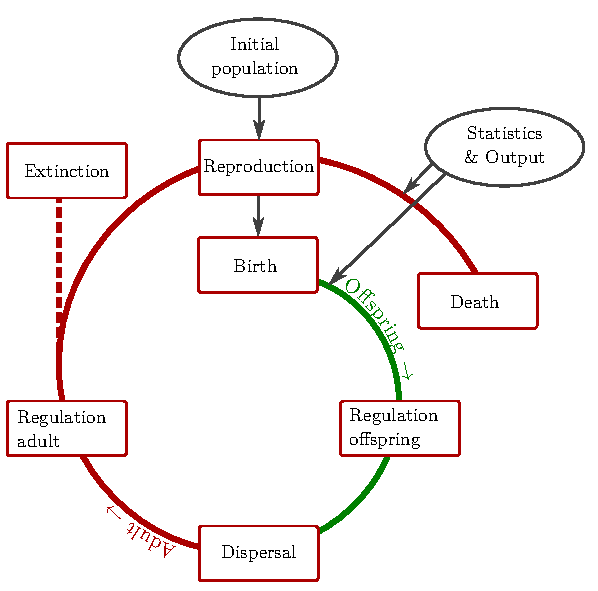
\includegraphics[width=0.80\textwidth]{life_cycle.pdf}
    \label{fig:life-cycle}
\end{figure}
\begin{description}
\item \textbf{\hyperref[sec:MatingSystem]{1 : Breeding.}} Adults mate and may produce offspring. By default, selection acts at this stage.
\item \textbf{\hyperref[sec:Death]{2 : Death.}} Adults are removed from the population. Only the juveniles remain in the model.
\item \textbf{\hyperref[sec:RegulationOffspring]{3 : Regulation.}} Reduce if necessary the population size to carrying capacity on each patch before dispersal. 
\item \textbf{\hyperref[sec:Dispersal]{4 : Dispersal.}} Individual can migrate to other patches and become adults. 
\item \textbf{\hyperref[sec:RegulationAdults]{5 : Regulation.}} Reduce if necessary the population size to carrying capacity on each patch after dispersal. 
\item \textbf{\hyperref[sec:Extinction]{6 : Extinction.}} Due to stochastic events populations may go extinct.
\end{description}
Moreover, during each cycle,  two events are called between breeding and death, allowing to save informations about the simulation.  Notice that at this moment, both adults and Juveniles are present, the main difference between both being that the adult might come from another patch while Juvenile not. 
\begin{description}
\item \textbf{\hyperref[sec:SummaryStatistics]{Statistics}} It is the stage were summary statistics can be computed for adults and juveniles.
\item \textbf{\hyperref[sec:RawData]{Output}} Genotypes and/or phenotypes can be dumped to files for adults and/or juveniles.
\end{description}
Most of the life cycle events are described in the following pages. However, the dispersal is included in the chapter about demography,  section \ref{sec:Dispersal}. All the information about statistics and output is also given in a separate chapter \ref{chap:OutputsAndStatistics}.


\section{Mating system}\label{sec:MatingSystem}
This stage performs mating and reproduction following the selected mating system. The implemented reproduction model in quantiNemo consists of two steps: First, for each patch, the number of offspring to be produced is defined. This number of offspring depends on the parameter \textsf{mating\_nb\_offspring\_model} and if selection acts at this stage also on the level of selection (see parameter \textsf{selection\_level}). In a second step, parents are randomly assigned for each offspring (parents are coming form the same patch). This assignment of the parents to the offspring depends on the mating system (parameter \textsf{mating\_system}) and on the fitness of the parents if selection acts. Thereby, adults with a higher fitness have on average a higher reproductive success. By default, selection acts at the reproductive success. Adults are not removed at this stage (adults are removed in the event \textsf{death}). The following parameters allow to parametrize this life cycle event:
 
\begin{description}

\item[mating\_system\index{mating\_system}]\textbf{[0-6] (default: 0)}\\
Five general mating systems are implemented in quantiNemo. The assignment of the parents to the offspring is random depending on the fitness of the local parents (if no selection acts all individuals have a fitness of 1). Adults with a higher fitness have on average a higher reproductive success):

\begin{description}
\item [0~:~random mating (hermaphrodite).] For each offspring, two hermaphrodite parents are randomly assigned. With probability $1/N$ these two hermaphrodites are identical which leads to selfing. Females are used to simulate hermaphrodites. 

\item [1~:~selfing (hermaphrodite).] For each offspring, a hermaphrodite is randomly assigned to self-fertilize. The parameter \textsf{mating\_proportion} allows setting the proportion of outcrosses. quantiNemo controls that the proportion of outcrosses is met, \textit{i.e.} that outcrossing does not result by chance ($1/N$) in selfing. Females are used to simulate hermaphrodites.

\item [2~:~cloning (hermaphrodite).] This mating system is identical to the model selfing but without any recombination. The genotype of the offspring is identical to the genotype of the mother (only females are simulated) except for changes due to mutations. The parameter \textsf{mating\_proportion} allows setting the proportion of sexual reproduction (random mating). Females are used to simulate hermaphrodites.

\item [3~:~random mating (promiscuity).] This is random mating with two sexes. For each offspring a father and a mother are randomly assigned.

\item [4~:~polygyny.] Depending on the parameter \textsf{mating\_males} only one (default) or several males per patch may reproduce. This fixed number of reproductive males are selected randomly depending on their fitnesses, \textit{i.e.} the reproductive males have on average a higher fitness. Then for each offspring, a mother and one of these reproductive males are randomly assigned depending on their fitnesses. Thus reproductive males with higher fitnesses have a higher reproductive success among the reproductive males. If no selection acts the reproductive males are randomly chosen (all males have the same probability) and each male has the same probability to father an offspring. The parameter \textsf{mating\_proportion} allows to set the proportion of random matings between any male and female, \textit{i.e.} also males of the non-reproductive group may get the chance to reproduce.

\item [5~:~monogamy.] For each female a male is randomly assigned to be its partner for all offspring. If there are fewer females than males present in the patch, not all males will mate. In contrast, if there are more females than males present in the patch, males may belong to several mating pairs. For each offspring, a parent pair is randomly assigned depending on the fitness of the female (if no selection acts the parent pairs have the same probability to be selected). Thus parent pairs, where the females have a higher fitness have on average a higher reproductive success. The parameter \textsf{mating\_proportion} allows setting the proportion of random matings.

\item [6~:~no mating/reproduction.] In this case no mating or reproduction occurs, \textit{i.e.} this life cycle event is skipped. This option allows using quantiNemo as a statistical package. The input data may be passed as initial genotype files (ntrl or quanti) in the FSTAT format (see sections \ref{sec:InitialGenotypes}). The number of generations has to be set to one since a simulation without any mating and reproduction does not make sense.

\end{description}

Models and their specific parameters\\

\begin{tabular}{ll}
 \hline model & additional parameters \\ 
 \hline  0~:~random mating (herma.) & \\
 1~:~selfing(herma.)      & mating\_proportion \\
 2~:~cloning (herma.)      & mating\_proportion \\
 3~:~random mating (prom.) & sex\_ratio \\
 4~:~polygyny              & sex\_ratio / mating\_proportion / mating\_males \\
 5~:~monogamy              & sex\_ratio / mating\_proportion \\
 6~:~no mating/reproduction & \\
 \hline
\end{tabular}

\item[mating\_proportion\index{mating\_proportion}] \textbf{[decimal] (temporal/default: 1)}\\
This parameter allows specifying the ratio of a special mating system (selfing, cloning, polygyny, or monogamy) in relation to random mating. A value of 1 (default) means that only the special mating occurs and a value of 0 means that only random mating occurs. For example, if we want to simulate a plant with a selfing rate of 90\% we have to set the parameter \textbf{mating\_system} to 1 (selfing) and this parameter \textbf{mating\_proportion} to 0.9. These settings will lead to 90\% selfing and 10\% random mating. Note, that quantiNemo controls that the ratio is met, \textit{i.e.} that selfing does not occur by chance (probability would be $1/N$) when random mating should occur.

\item[mating\_males\index{mating\_males}] \textbf{[integer] (default: 1)}\\
This parameter sets the number of males that will be available for mating within each patch. The parameter will only be used if the mating system is polygyny (parameter \textsf{mating\_system} set to 4). The range of values is between 1 (a single male mates) and the carrying capacity of the males (all males may mate).

\item[sex\_ratio\index{sex\_ratio}] \textbf{[decimal] (default: 1)}\\
This parameter allows to specify the ratio of males to females of the offspring in a patch. If hermaphrodites are simulated (parameter \textsf{mating\_system} is set to 0, 1 or 2) the sex ratio is not considered, respectively set to 0 (females are used to simulate hermaphrodites).

\item[sex\_ratio\_threshold\index{sex\_ratio\_threshold}] \textbf{[decimal] (default: "")}\\
By default, the sex of an individual is randomly assigned depending on the specified sex ratio (see parameter \textsf{sex\_ratio}). If the parameter \textsf{sex\_ratio\_threshold} is set the sex of an offspring is determined by the phenotype of the first quantitative trait of the offspring. The argument specifies the threshold above which an individual becomes a male. If this parameter is set the parameter \textsf{sex\_ratio} is not considered. Note, that when using this parameter the phenotype has to be defined at the offspring stage, thus the parameter \textsf{quanti\_environmental\_proportion} has to be set to 0. Using this parameter it is possible to simulate sex chromosomes.  

\end{description}


\section{Death}\label{sec:Death}
This life cycle event simply removes the adults present.


\section{Regulation offspring}\label{sec:RegulationOffspring}
This event performs population regulation before dispersal, \textit{i.e.} at the offspring stage. This life cycle event allows to regulate the population sizes down to carrying capacity. In fact the regulation should only be used if there is no regulation at the reproduction stage, \textit{i.e.} if the parameter \textsf{mating\_nb\_offspring\_model} is set to 1 (keep number), 2 (fecundity), 3 (fecundity stochastic) or 4 (fecundity binomial). If the parameter \textsf{selection\_position} is set to 2 then selection acts at this stage. In this case the following parameter is ignored and offspring regulation happens following the parameter \textsf{selection\_level}.  
\begin{description}
\item[regulation\_model\_offspring\index{regulation\_model\_offspring}] \textbf{[0,1] (default: 0)}
\begin{description}
\item[0~:~no regulation.] No population size regulation takes place at the offspring stage, \textit{i.e.} overcrowding can occur.
\item[1~:~random regulation.] For each patch quantiNemo regulates the population size down to its carrying capacity if the population size exceeds carrying capacity. Individuals are thereby randomly removed. No regulation takes place if the population size is lower than carrying capacity.
\end{description}
\end{description}



\section{Regulation adults}\label{sec:RegulationAdults}
This event performs population regulation after dispersal, \textit{i.e.} at the adult stage. Due to asymmetric dispersal, some patches may be overcrowded. This life cycle event allows regulating the population sizes down to carrying capacity. If the parameter \textsf{selection\_position} is set to 3 then selection acts at this stage. In this case, the following parameter is ignored and offspring regulation happens following the parameter \textsf{selection\_level}.  

\begin{description}
\item[regulation\_model\_adults\index{regulation\_model\_adults}] \textbf{[0,1] (default: 0)}
\begin{description}
\item[0~:~no regulation.] No population size regulation takes place at the adults stage, \textit{i.e.} overcrowding can occur.
\item[1~:~random regulation.] For each patch quantiNemo regulates the population size down to its carrying capacity if the population size exceeds carrying capacity. Individuals are thereby randomly removed. No regulation takes place if the population size is lower than carrying capacity.
\end{description}
\end{description}

\section{Extinction}\label{sec:Extinction}
This event allows to randomly wipe out populations entirely or partially. It is useful to simulate different types of event like diseases or natural disasters.   The probability that a population goes extinct is specified by the parameter \textsf{extinction\_rate} and the parameter \textsf{extinction\_rate\_survival} specifies how much a population is affected. If the extinction rate is zero this event is skipped.

\begin{description}
\item[extinction\_rate\index{extinction\_rate}] \textbf{[decimal/matrix] (temporal/default: 0)}\\
Extinction probability of a patch at each generation. Can be specified for each patch separately.

\item[extinction\_rate\_survival\index{extinction\_rate\_survival}]\hspace*{\fill}\\
\vspace{-9mm}
\item[extinction\_rate\_survival\_fem\index{extinction\_rate\_survival\_fem}]\hspace*{\fill}\\
\vspace{-9mm}
\item[extinction\_rate\_survival\_mal\index{extinction\_rate\_survival\_mal}] \textbf{[decimal/matrix] (temporal/default: 0)}\\
These parameters specify how a population is affected when it is hit by an extinction event. By default (value 0) the entire population is wiped out. If the parameter is not 0 then at an extinction event individuals will survive. The effect on the population may be defined absolutely if the value is 1 or larger (e.g. 5 individuals survive), relatively if the value is between 0 and 1 (e.g. 10\% of the individuals survive), or a combination of relatively and absolutely when specified patch specific  using a matrix. The survival rate may be specified for each sex separately or in common. Note that in this later case the values will be used for each sex separately, e.g. if the parameter \textsf{extinction\_rate\_survival} is set to 0.4, then 40\% of the females and 40\% of the males will survive if an extinction event happens and if set to 100 and two sexes are simulated 50 females and 50 males will survive.

\end{description}


%%%%%%%%%%%%%%%%%%%%%%%%%%%%%%%%%%%%%%%%%%%%%%%%%%%%%%%%%%%%%%%%%%%%%%%%%%%%%%%%%%%%%%%%%%%%%%%%%%%%%%%%%%%%%%%%%%%%%%%%%%%%%%%%%%%%%%
\newpage
\chapter{Demography}\label{chap:Demography}
This section describes how to simulate a specific demographical scenario, changing the initial number of individual in each patch, the patch capacity, the migration model and how the population growth with time. 
\section{Dimensions}
\begin{description}

\item[generations\index{generations}]\textbf{[integer]}\\
Number of generations to perform per replicate. This parameter is mandatory, and has no default.
\item[patch\_capacity\index{patch\_capacity}]
\textbf{[integer/matrix] (temporal)}\\
Carrying capacities of the patches. This parameter is mandatory, and has no default.

 If all patches have the same carrying capacities a single number as argument is sufficient to specify the carrying capacities. To set the carrying capacities individually for each patch a matrix is needed. Note, using a two-dimensional matrix with two columns allows addressing directly a patch and thus specifying carrying capacity explicitly for this patch (e.g. \textit{\{\{patchID value\}\{patchID value\}...\}}), while all not specified patches will have a carrying capacity of 0. 


\item[patch\_capacity\_fem\index{patch\_capacity\_fem}]\hspace*{\fill}\\
\vspace{-9mm}
\item[patch\_capacity\_mal\index{patch\_capacity\_mal}]\textbf{[integer/matrix] (temporal)}\\
The carrying capacities may vary among sexes, patches, and time. The carrying capacities have to be specified either for each sex separately (parameters \textsf{patch\_capacity\_fem} and \textsf{patch\_capacity\_mal}), or for both sexes together (parameter \textsf{patch\_capacity}). In the first case both sex specific parameters have to be set if two sexes are simulated. In the latter case the carrying capacities for females and males are assumed to be identical, \textit{i.e.} the carrying capacity of females and males is $patch\_capacity/2$. If hermaphrodites are simulated the parameters \textsf{patch\_capacity} and \textsf{patch\_capacity\_fem} are identical. In case all three parameters are set, only the sex specific parameters will be used as they are more informative.
\item[patch\_number\index{patch\_number}] \textbf{[integer] (default: 1)}\\ 
This parameter specifies the number of patches in the metapopulation.
\end{description}
\section{Initialization}
This section allows specifying how the metapopulation is initialized. The population size of the patches may be set in three different ways. Also, the genotypes of the individuals of the initial populations may be set differently. By default, \textit{i.e.} if no special parameters of this section are defined, the initial population size of each patch corresponds to its carrying capacity (see parameter \textbf{patch\_capacity} above). If the initial population sizes deviate from the carrying capacities the parameter \textbf{patch\_ini\_size} allows setting the initial population size for each patch separately. Finally, it is possible to define the genotypes of each individual explicitly using an FSTAT file \citep{Goudet_1995}. By doing this also the initial population sizes are defined. For details please have a look at the parameters \textbf{quanti\_ini\_genotypes} and \textbf{ntrl\_ini\_genotypes} in the chapter about \hyperref[chap:Genetics]{genetic}. If a genotype file is present the initial population sizes are defined using this file.

\begin{description}

\item[patch\_ini\_size\index{patch\_ini\_size}]\hspace*{\fill}\\
\vspace{-9mm}
\item[patch\_ini\_size\_fem\index{patch\_ini\_size\_fem}]\hspace*{\fill}\\
\vspace{-9mm}
\item[patch\_ini\_size\_mal\index{patch\_ini\_size\_mal}]\textbf{[integer/matrix]}\\
These parameters allow to set the initial population sizes of the patches, \textit{i.e.} the populations sizes present at the beginning of the simulation. These parameters are optional. If none of these parameters is set, \textit{i.e.} the initial population sizes are not set, the simulation will start with all the population sizes set at carrying capacity. The initial population sizes may vary among sexes, and patches. The initial population sizes have to be specified either for each sex separately (parameters \textsf{patch\_ini\_size\_fem} and \textsf{patch\_ini\_size\_mal}), or for both sexes together (parameter \textsf{patch\_ini\_size}). In the first case both sex specific parameters have to be set if two sexes are simulated. In the latter case the initial population sizes for females and males are assumed to be identical, \textit{i.e.} the initial population size of females and males is $patch\_ini\_size/2$. If hermaphrodites are simulated the parameters \textsf{patch\_ini\_size} and \textsf{patch\_ini\_size\_fem} are identical. In case all three parameters are set the sex specific parameters will be used as they are more informative. To set the initial population sizes individually for each patch a matrix is needed. The matrix is adjusted to the number of patches if necessary (see section \ref{matparam}). If all patches have the same initial population sizes a single number as argument is sufficient to specify the initial population sizes.

Note, using a two dimensional matrix with two columns allows addressing directly a patch and thus specifying the initial population size for this patch (e.g. \textit{\{\{patchID value\}\{patchID value\}...\}}), while all not specified patches will have an initial population size of 0.
\end{description}
\section{Population growth}
\begin{description}
\item[mating\_nb\_offspring\_model\index{mating\_nb\_offspring\_model}] \textbf{[0-9] (default: 0)}\\
This parameter specifies how the total number of offspring ($N_{Off}$) produce at each generation is determined. 

The actual number of offspring also depend on the selection level (see parameter \textsf{selection\_level}). In case of soft selection, only the parameter \textsf{mating\_nb\_offspring\_mode} is taken into account.  However, if the selection is hard, then the total number of offsping is computed taking also into account the mean fitness of the population. Finally, in the case of metapopulation selection, the total number of offspring for the entire population is computed using only  \textsf{mating\_nb\_offspring\_model}, but they are then reassigned to specific patches depending on the mean fitness of each patch. 

\item [0~:~carrying capacity.]  \[ N_{Off} = K \]
The total number of offspring ($N_{Off}$) is set to the carrying capacity ($K$, parameter \textsf{patch\_capacity}) of the patch or the metapopulation, respectively.
\item [1~:~keep number.] \[ N_{Off} = N \]
The total number of offspring ($N_{Off}$) corresponds to the number of adults ($N$), \textit{i.e.} the number of individuals is kept constant. Note that a regulation of the patch densities after dispersal can lead to an unwanted continuing reduction of the entire metapopulation size. 
\item [2~:~fecundity.]  \[ N_{Off} = Poisson(N_{F}f) \]
The number of offspring ($N_{Off}$) depends on the mean fecundity of the females ($f$) defined by the parameter \textsf{mean\_fecundity}.
\item [3~:~fecundity simple.] \[ N_{Off} = round(N_{F}f) \]
A simplified version of point 2 assuming that the fecundity is always the same (no fluctuations). This simplification speeds up computation and is acceptable for a wide range of simulation problems.
\item [4~:~fecundity binomial.] \[ N_{Off} = floor(N_{F}f)+Binomial(N_{F}f-floor(N_{F}f),1) \]
Similar to point 3, but the rounding is replaced by random rounding with probability equal to the decimal part of the number, \textit{i.e.} drawing a random number in a binomial distribution with probability equal to the decimal part of the number.
\item [5~:~fecundity limited.] 
\[ N_{Off}= Poisson(N_{F}f) \]
\[ if(N_{Off}>K) N_{Off}=K \]
Same as point 2, but if the new population size exceeds carrying capacity the population size is down-regulated to carrying capacity.
\item [6~:~fecundity simple \& limited.]
\[ N_{Off}=round(N_{F}f) \]
\[ if(N_{Off}>K) N_{Off}=K \]
Same as point 3, but if the new population size exceeds carrying capacity the population size is down-regulated to carrying capacity.
\item [7~:~fecundity binomial \& limited.]
\[ N_{Off}=floor(N_{F}f)+Binomial(N_{F}f-floor(N_{F}f),1) \]
\[ if(N_{Off}>K) N_{Off}=K \]
Same as point 4, but if the new population size exceeds carrying capacity the population size is down-regulated to carrying capacity.
\item [8~:~logistic regulation.] \[ N_{Off} = \frac{NK(1+r)}{N(1+r)-N+K} \]
The total number of offspring ($N_{Off}$) is logistically regulated following the discrete-time function of \citet{Beverton_1957} and depends therefore on the carrying capacity ($K$) and on the parameter \textsf{growth\_rate} ($r$). 
\item [9~:~stochastic logistic regulation.] \[ N_{Off} = Poisson\left(\frac{NK(1+r)}{N(1+r)-N+K}\right) \] 
Same as point 8, but the computation of the total number of offspring has a stochastic component.
\end{description}

Models and their specific parameters\\


\begin{tabular}{ll}
 \hline model                        & additional parameters \\ 
 \hline
 carrying capacity (0)               & \\
 keep number (1)                     & \\
 fecundity (2-7)                     & mean\_fecundity\\
 logistic regulation (8-9)           & growth\_rate\\
 \hline
\end{tabular}
\begin{description}
\item[mean\_fecundity\index{mean\_fecundity}] \textbf{[decimal] (temporal)}\\
This parameter specifies the mean female fecundity. The parameter is mandatory (and only used) if the fecundity of the female specifies the number of offspring (i.e. parameter \textsf{mating\_nb\_offspring\_model} set to 2 or 3).

Note that for population of hermaphrodites (\textsf{mating\_system} 0,1 or 2), a mean fecundity of 1 leads to constant population size, while in dioecious systems (\textsf{mating\_system} 3,4 or 5), it's a mean fecundity of 2 which leads to a constant population size.  

\item[growth\_rate\index{growth\_rate}] \textbf{[decimal] (temporal)}\\
This parameter is mandatory (and only used) if logistic regulation is used to specify the number of offspring (i.e. parameter \textsf{mating\_nb\_offspring\_model} set to 4 or 5). It specifies the growth rate \textit{r} of the population using the discrete-time function of \citet{Beverton_1957}.  

When the population is much smaller than the carrying capacity, $r +1$ can be thought as the mean number of offspring created per individual. So if $r=0$, the mean number of offspring per individual is $1$, and the population size is constant. 
\end{description}


%%%%%%%%%%%%%%%%%%%%%%%%%%%%%%%%%%%%%%%%%%%%%%%%%%%%%%%%%%%%%%%%%%%%%%%%%%%%%%%%%
\section{Dispersal}\label{sec:Dispersal}
During its life cycle, each individual might migrate from one patch to another. Several dispersal models are available (see parameter \textsf{dispersal\_model}). It is also possible to specify a dispersal matrix, which will have precedence over other dispersal parameters. After dispersal, individuals become adults. By default (if none of the following parameters are set) individuals do not disperse among patches.

\begin{description}
\item[dispersal\_rate\index{dispersal\_rate}]\hspace*{\fill}\\
\vspace{-9mm}
\item[dispersal\_rate\_fem\index{dispersal\_rate\_fem}]\hspace*{\fill}\\
\vspace{-9mm}
\item[dispersal\_rate\_mal\index{dispersal\_rate\_mal}]\textbf{[decimal/matrix] (temporal/default: 0)}\\
These parameters allow setting the emigration rate (if the argument is between 0 and 1 (1 included), or the number of emigrants (if the argument is an integer). 

If the argument is a single value the dispersal model used depends on the other parameters of this section. But it is also possible to specify the dispersal rate explicitly between each pair of patches (for both directions) if the argument is a matrix. A dispersal matrix has precedence over all other dispersal settings. The matrix must be \texttt{patch\_number} x \texttt{patch\_number} in dimensions. Each $d_{ij}$ element of this matrix is the dispersal probability from patch $i$ to patch $j$, where $i$ specifies the row and $j$ the column of the matrix. Consequently, the values in a row must sum up to 1 (if the row do not sum up to 1 the proportion of residents (diagonal) will be adjusted and a warning returned). The dispersal rates can either be specified for both sexes in general or for each sex separately. If the dispersal rates are sex specific the dispersal rates for both sexes have to be specified and they have to be in the same format (matrix or a single dispersal rate). Sex specific dispersal rates have precedence over a general dispersal rate. Note, that the dispersal matrix has to be fully specified, \textit{i.e.} the matrix is not adjusted to the number of patches as for other parameters. 

\item[dispersal\_model\index{dispersal\_model}] \textbf{[0-4] (default: 0)}\\
The following dispersal models are available:
\begin{description}
\item[0~:~Migrant-pool Island model.] If the dispersal rate is $m$ and the number of patches is $n_{p}$, the probability to disperse to any $n_{p}-1$ non-natal patch is $\frac{m}{n_{p}-1}$ while the probability to stay at home is $1-m$.

\item[1~:~Propagule-pool Island model.] In that modified version of the Island model, emigrants tends to move between patches in group. More precisely, for each patch, a fraction of individual of size $m\varphi$ will migrate altogether to another randomly picked patch. Another fraction of emigrant,  $m(1-\varphi)$,  will migrate to all others patches. Finally,  a fraction of $1-m$ individuals will stay at home.

\item[2~:~1D Stepping-Stone model.] In the one dimensional Stepping Stone model patches are placed on a line and migrants can only move to one of the two adjacent patches. If the dispersal rate is $m$, the probability to disperse to one of the adjacent patches is $m/2$ while the probability to stay at home is $1-m$. The parameter \texttt{dispersal\_border\_model} allows to specify how to treat the border patches.   

\item[3~:~2D Stepping-Stone model.] In the two dimensional Stepping-Stone model patches are placed on a grid (or lattice) and migrants can move to 4 or 8 adjacent patches (set by the \textsf{dispersal\_lattice\_range} parameter below). If the dispersal rate is $m$, the probability to disperse to one of the adjacent patches is $m/4$ or $m/8$ depending on the parameter \textsf{dispersal\_lattice\_range}, while the probability to stay at home is $1-m$. The parameter \textsf{dispersal\_border\_model} allows to specify how to treat the border patches and the parameter \textsf{dispersal\_lattice\_dims} allows specifying the dimensions of the grid.   

\end{description}

Models and their specific parameters\\
\begin{tabular}{ll}
 \hline model & additional parameters \\ 
 \hline
 0~:~Migrant-pool Island    & \\
 1~:~Propagule-pool Island  & dispersal\_propagule\_prob\\
 2~:~1D Stepping-Stone      & dispersal\_border\_model\\
 3~:~2D Stepping-Stone      & dispersal\_border\_model / dispersal\_lattice\_range / \\
                            & dispersal\_lattice\_dims\\
 \hline
\end{tabular}


\item[dispersal\_lattice\_range\index{dispersal\_lattice\_range}] \textbf{[0,1] (default: 0)}\\
This parameter sets the number of neighboring patches used for dispersal. The dispersal probabilities to these adjacent patches are $m/4$ in the first case and $m/8$ in the second. This parameter is only used in the 2D Stepping-Stone model (parameter \textsf{dispersal\_model} set to 3).
\begin{description}
\item[0~:~4 neighbors.]4 adjacent patches (up, down, left and right)
\item[1~:~8 neighbors.]8 adjacent patches (as before plus the diagonals)
\end{description}

\item[dispersal\_border\_model\index{dispersal\_border\_model}] \textbf{[0-2] (default: 0)}\\
This parameter specifies how the patches at a border of the Stepping Stone model should be treated:
\begin{description}
\item[0~:~Circle/Torus.] In the 1D Stepping-Stone model the first and last patches are connected to each other by migration leading to a circle. In the 2D Stepping-Stone model individuals of an edge patch may migrate to the other side leading to a torus (donut world). This means that there are no edges, eliminating any such effects.
\item[1~:~Reflective boundaries.] The borders are reflective. Dispersers from the border patches cannot move beyond the border. Border cells have thus less cells connected to them and their dispersal probabilities to the adjacent patches are higher (e.g. $m$ for the 1D Stepping-Stone model, $m/3$ (corners $m/2$) for the 2D Stepping-Stone model with four adjacent cells, and $m/5$ (corners $m/3$) for the 2D Stepping-Stone model with eight adjacent cells). No dispersers are lost.
\item[2~:~Absorbing boundaries.] Dispersers of the border patches are lost if they choose to move beyond the border. The dispersal probabilities of a border patch are not modified. 
\end{description}

\item[dispersal\_lattice\_dims\index{dispersal\_lattice\_dims}] \textbf{[matrix]}\\
This parameter allows to specify the length and width of the 2D Stepping-Stone lattice (only used when \textsf{dispersal\_model} is set to 3). The argument is an integer matrix with two values. The first value stands for the number of rows, and the second value for the number of columns. The product of the two values results in the number of patches and thus must match the parameter \textsf{patch\_number}. If the parameter is not set quantiNemo assumes that the 2D Stepping-Stone lattice is quadratic. If this is not possible due to the number of patches an error is returned. 


\item[dispersal\_propagule\_prob\index{dispersal\_propagule\_prob}] \textbf{[decimal] (temporal/default: 1)}\\
This parameter is only used for the Propagule-pool Island model (parameter \textsf{dispersal\_model} set to 1). It specifies the probability that a migrant will move to the propagule-assigned patch, \textit{i.e.} this is also the proportion of emigrants of a patch which migrate to the same non-natal patch. A probability of 1 means that all emigrants migrate to the same non-natal patch, while a value of 0 means that all emigrants migrate to any patch, but the natal and the propagule patch. 

\end{description}

\subsection{Density dependent dispersal rate}
By default, the dispersal rate is not influenced by the population size/density of the natal patch. The following parameters allow describing a situation where the migration depends on the density of the natal patch: 

 \begin{description}
\item[dispersal\_rate\_model\index{dispersal\_rate\_model}] \textbf{[decimal] (temporal/default: 0)}\\
this parameter define how the dispersal rate is set.
\begin{description}
                  \item[0~:~Flat rate.] The rate is constant and does not depend of the density
                  \item [1~:~Dependant rate 1] Rate depend on density following the relation $ m_{\text{eff}} = \frac{me}{N}*(N-K(1-\exp(-N/K)))$, where $m$ is the migration rate, $K$ the patch capacity, $N$ the number of individual on the patch before migration and $e$ the Euler constant. Notice that in this case, the migration rate is exactly $m$ (parameters \textsf{dispersal\_rate}) when the density is one.
                   \item [2 ~:~Dependant rate 2] Rate depend on density following the relation $m_{\text{eff}} =\frac{(N-K(1-\exp(-N/K)))}{N}$. Notice that in this case, the migration rate specified using the parameter \textsf{dispersal\_rate} is not used, and instead the migration rate is smoothly adjusted so that the density after dispersal is always smaller than one. 
\end{description}
\end{description}


\chapter{Genetics}\label{chap:Genetics}
\section{Introduction}
QuantiNemo allows the simulation of quantitative traits as well as neutral markers, both related by a common genetic map so that processes like linkage disequilibrium and genetic hitchhiking can be simulated easily. More precisely, quantiNemo allows to simulate neutral markers, such as microsatellites or SNPs with different mutation models (K allele and Stepwise). Quantitative trait under selection pressure composed of various loci can also be added to the same simulation. In this chapter, we explain how to define loci and traits, locate them in a map, set an initial genotype and choose a mutation model for them.

Most of the parameter and behaviour are the same for neutral and quantitative traits (except of course that quantitative traits are under selection, but this will be cover in the next chapter). The main difference is that neutral trait's parameters are defined with a \textsf{ntrl\_} in front while quantitative traits are specified with  \textsf{quanti\_}. In the case where the parameters have the same meaning for neutral and quantitative traits, the \textsf{(ntrl/quanti)\_parameter} notation will be used, which should be read as the existence of two parameters, one \textsf{ntrl\_parameter} and another one \textsf{quanti\_parameter}. If differences are present  ,as for example in the mutations models, both parameters are explained separately. 
\section{Settings loci}
\label{sec:SettingsLoci}
\begin{description}
\item[(ntrl/quanti)\_loci\index{ntrl\_loci}\index{quanti\_loci}] \textbf{[integer]}\\
This parameter specifies the number of neutral/quantitative loci per individual per traits (by default, there is only one trait). This parameter is mandatory for the simulation of a neutral/quantitative locus \textit{i.e.} it is necessary as soon as we want to study genetic effect. If this parameter is not present, the other parameters related to genetics make no sense and will not be loaded. 

\item[(ntrl/quanti)\_all\index{ntrl\_all}\index{quanti\_all}] \textbf{[1-256/matrix] (default: 255)}\\
This parameter specifies the maximal possible number of alleles per locus. Using a matrix it is possible to specify this number for each locus of a trait separately. For quantitative trait, it is recommended to take a odd number of allele in order to have a "central allele", but it's not mandatory. 
\end{description}

\begin{description}
\item[\label{allelicFile}(ntrl/quanti)\_allelic\_file\index{ntrl\_allelic\_file}\index{quanti\_allelic\_file}]  \textbf{[string] (default: "")} \\
This parameter allows to pass the name of a file containing allele informations, such as the initial allele frequencies, and/or the mutation probability to an allele. The number of alleles and loci has to be in line with the parameters \textsf{(ntrl/quanti)\_loci} and \textsf{(ntrl/quanti)\_all}. The information can be set globally for all loci, if they have the same specifications, or for each locus separately. The allelic files for neutral markers and for quantitative trait have similar format except for two columns:

\begin{lstlisting}[frame=single]
#Allelic file 
###############
[FILE_INFO]{
  col_locus 1
  col_allele 2
  col_allelic_value 3
  col_mut_freq 4
  col_ini_freq 5
}

#locus  allele  value   mut_freq  ini_freq  
1       1       -1.    0.2       {0  0.33}
1       2       0    0.4       {0  0.33}
1       3       2.     0.4       {1  0.33}
2       1       -1.      0.33       {0  0.33}
2       2       0.      0.33       {0  0.33}
2       3       1.       0.33       {1  0.33}
\end{lstlisting}

The file has to start with a file information box \textsf{[FILE\_INFO]}\{...\}. This box contains the information of the structure of the following table allowing a flexible structure of the table. For example the order of the columns in the table may vary, or columns may be ignored. The file information box starts with the keyword \textsf{[FILE\_INFO]} and the information is enclosed by brackets "\{...\}". Line by line the index of the columns to be read have to be declared. Thereby a keyword for the specific setting is followed by the column index (the ordering starts with 1). The following column keywords are available:
\begin{description}
\item [col\_locus] This keyword specifies the column containing the locus index. If this column is not declared in the file information box, quantiNemo will use the same settings for all loci. In this case, the length of the table must meet the number of alleles (\textsf{ntrl\_all}). If this keyword is declared the length of the table must meet the number of alleles times the number of loci (\textsf{ntrl\_loci} * \textsf{ntrl\_all}).   
\item [col\_allelic\_value] This keyword specifies the column containing the allelic effects, \textit{i.e.} how an allele contribute to the value of a trait (c.f. \ref{sub:AllelicEffects}). If this column is not set the allelic effects will be equally spaced on a range which depend of the parameter \textsf{quanti\_all\_effect\_var}. Since only quantitative trait have an allelic value, this column is only available for quantitative traits.
\item [col\_allele] This keyword specifies the column containing the allele index. This column is mandatory. The index of the allele goes from 1 to \textsf{quanti/ntrl\_loci}.
\item [col\_mut\_freq] This keyword specifies the column containing the mutation probabilities, \textit{i.e.} the probability to mutate to this allele when a mutation occurs. The behaviour of this mutation probability depends on the mutation model (see parameter (\textsf{ntrl\_mutation\_model}).This keyword is only available for quantitative traits. 
\item [col\_ini\_freq] This keyword specifies the column containing the initial frequencies of the alleles. This column allows to explicitly set the allele frequencies at the start of a simulation. The frequencies can be set for each patch separately using a matrix. In the example above, individuals of the first population are initially fixed for the allele 3 at the first locus as well as at the second locus. In the second population, all alleles have the same initial frequency of 0.2. Note, that the matrix is adjusted in length if the number of populations does not correspond to the length of the matrix. If this column is not given the initial allele frequencies are set globally depending on the parameter \textsf{ntrl\_ini\_allele\_model}.
\end{description} 
Note, that as in all input files for quantiNemo it is possible to define comments (also in the file information box) using the hash character: '\#' or '\#/ ...any text... /\#'.
\end{description}


\section{Initial genotypes}\label{sec:InitialGenotypes}
There are several methods to set the allele frequencies or even the genotypes of the individuals at the start of a simulation (initialization). The genotypes of the individuals may be set using an FSTAT file \citep{Goudet_1995} (parameter \textbf{(ntrl/quanti)\_ini\_genotypes}). If such a FSTAT file is not present the genotypes are randomly drawn following the explicitly set allele frequencies in the allelic file (see parameter \textbf{(ntrl/quanti)\_allelic\_file} and especially column keyword \textbf{col\_ini\_freq}). If the allele frequencies are not set explicitly in the allelic file the initialization is performed following the parameter \textbf{(ntrl/quanti)\_ini\_allele\_model}.  

\begin{description}
\item[(ntrl/quanti)\_ini\_genotypes\index{quanti\_ini\_genotypes}\index{ntrl\_ini\_genotypes}] \textbf{[string] (default: "")}\\
This parameter allows to specify a name of an FSTAT file \citep{Goudet_1995} containing the initial genotypes of the individuals for each population. If such a file is present the initialization of the metapopulation is done solely by this file ignoring the parameters \textbf{(ntrl/quanti)\_ini\_allele\_model} and \textbf{patch\_ini\_size}. A single FSTAT file is needed for all quantitative traits together containing the total number of loci of all quantitative traits together. Note, that quantiNemo allows to output an appropriate file for any generation (see parameter \textbf{(ntrl/quanti)\_save\_genotype}). This allows resuming a simulation, to generate tailored initial conditions, or to continue a simulation with modified settings. If the parameter \textbf{(ntrl/quanti)\_save\_genotype} is set to 2 an extended FSTAT file is generated. Also, this file may be used to initialize the metapopulation. In this case, quantiNemo overtakes the supplement information provided by the file, especially the sex and age of the individual, the index of the individual, its mother and father. Thus the supplement information allows resuming a simulation without the loss of the pedigree. Note, that for an entire resume of a simulation the genotypes of both neutral and quantitative traits have to be set. In this case the number of individuals per patch and the individuals supplement information (sex, age, individuals id, mothers id, fathers id must be in agreement with each other. 

\item[ntrl\_ini\_allele\_model\index{ntrl\_ini\_allele\_model}] \textbf{[0,1] (default: 0)}\\

If the genotypes or allele frequencies are not already defined in another way, the initialization of the genotypes may be either polymorphic, where the probability of each allele is identically or monomorphic, where all populations are fixed for a single allele.  

\begin{description}

\item[0~:~polymorph.] The populations are maximally polymorph with respect to allele frequencies at the start of a simulation.

\item[1~:~monomorph.] The populations are monomorphic with respect to allele frequencies at the start of a simulation. All individuals are fixed for a single allele, which is  the "middle" allele, \textit{i.e.} the allele with the index $\left\lfloor \textsf{ntrl\_all}/2\right\rfloor$.

\end{description}

\item[quanti\_ini\_allele\_model\index{quanti\_ini\_allele\_model}] \textbf{[0,1] (default: 0)}\\

If the genotypes or allele frequencies are not already defined in another way, the initialization of the genotypes may be either polymorphic, where the probability of each allele follow a normal distribution or monomorphic, where all populations are fixed for a single allele.  

\begin{description}

\item[0~:~polymorph.] The initial allele frequency is given by a (discretized) normal distribution with a variance given by the parameter \textbf{quanti\_allelic\_var}.

\item[1~:~monomorph.] The populations are monomorphic with respect to allele frequencies at the start of a simulation. All individuals are fixed for a single allele, which is  the "middle" allele, \textit{i.e.} the allele with the index $\left\lfloor \textsf{ntrl\_all}/2\right\rfloor$.

\end{description}
\end{description}

\section{Mutation}
Mutation rates may be defined for each locus individually by explicitly defining the individual mutation rates (parameter \textsf{(ntrl/quanti)\_mutation\_rate}) or by defining the gamma distribution from which the individual mutation rates are drawn (parameters \textsf{(ntrl/quanti)\_mutation\_rate} and \textsf{(ntrl/quanti)\_mutation\_var}). For quantitative trait, depending on the mutation model (parameter \textsf{quanti\_mutation\_model}) the mutant effect is the effect of the drawn allele (model 0), or the effect of the drawn allele is added to the current allelic effect to get the mutant effect (model 1). Using the allelic file (see section \ref{allelicFile}) it is possible to specify for each allele its effect and the probability to mutate to this allele given that there is a mutation. A minimal definition for mutations requires the setting of a common mutation rate (parameter \textsf{(ntrl/quanti)\_mutation\_rate} has a single value). In this case, all loci have the same mutation rate.

Note, that for all mutation models the number of alleles has to be odd if the allelic effects and the probabilities to mutate to the alleles given that there is a mutation are set automatically. In this case, also a warning will be drawn if the number of alleles is below 200, informing that this number of alleles may not well represent the normal distribution of the allelic effects.
the probability of each allele is identically or monomorphic, where all populations are fixed for a single allele.   
\begin{description}
\item[(ntrl/quanti)\_mutation\_rate\index{quanti\_mutation\_rate}\index{ntrl\_mutation\_rate}] \textbf{[decimal/matrix] (temporal/default: 0)}\\
This parameter specifies the mutation rate per locus and generation. If the argument is a single value the mutation rate for all loci is the same. By passing a matrix of mutation rates it is possible to set the mutation rate for every single locus individually. By default, no mutations occur.

\end{description}

\subsection{quantitative mutation model}
\begin{description}
\item[quanti\_mutation\_model\index{quanti\_mutation\_model}] \textbf{[0-3] (default: 0)}\\
This parameter allows specifying the mutation model, which define toward which allele we mutate when a mutation occurs. For quantitative traits, quantiNemo offers the possibility to simulate four very common models. Notice that the two first one are more common in quantitative traits while the two last ones are more meaningful for neutral markers, and are proposed here only as a "nice to have". 
\begin{description}

\item[0~:~RMM] (Random Mutation Model)\\
The new allele is randomly selected based on its index, following a Gaussian centred on the allele with an allelic value of 0 (the so-called central allele). The standard deviation of the Gaussian is the same as the one from which the allelic effects are drawn randomly (see parameter \textsf{quanti\_allelic\_var}). This simulates a system where every mutation has an allelic value normaly distributed around 0 with a variance of \textsf{quanti\_allelic\_var}.

If the probability to mutate to a given allele are given explicitly in the allelic file (see section \ref{allelicFile}), then, the new allele is randomly selected following the given distribution. 

\item[1~:~IMM] (Increment Mutation Model)\\
The new allele is randomly selected following a Gaussian which is centered around the allelic value of the previous allele, \textit{i.e.} the allele it is mutating from. The standard deviation of the Gaussian is the same as the one from which the allelic effects are drawn randomly (see parameter \textsf{quanti\_allelic\_var}). This simulates a system where every mutation has an effect which is normally distributed around the value of the previous allele.   

Note that with this model, the allelic values are equally space between $-20\sigma$ and $20\sigma$ instead of  $-6\sigma$ and $6\sigma$ ( where $\sigma$ is the square root of the parameter \textsf{quanti\_allelic\_var}) as it is the case for the other mutation model. This lets more freedom to the system to explore value far away from the starting point. It is therefore recommended to select a large number of allele to have a good representation of the possible values. 

If the probability to mutate to a given allele are given explicitly in the allelic file (see section \ref{allelicFile}), then, the new allele is randomly selecting following this given distribution. However, the distribution is re-centred around the current allele. If the new allele does not exist, no mutation is performed. 

\item[2~:~KAM] (K-Allele Model)\\
At each mutation, the existing allele is randomly exchanged by another allele within the range of alleles (i.e. $[1; quanti\_all]$) not taking into account any allelic effect. The probability to mutate to any allele is the same. In this case, the frequencies that are given in the allelic file (see section \ref{allelicFile}) are not taken into account. 

\item[3~:~SSM] (Single Step Mutation)\\
In the single step mutation, the new allele depends on the current allele index. When a mutation occurs the current allele is replaced by one of its neighbouring alleles. For example, if the allele with the index 12 mutates, it changes either to the allele with the index 13, or to the allele with the index 11. The boundaries are reflexive, \textit{i.e.} the allele index cannot exceed the range of alleles (i.e. $[1; ntrl\_all]$). Notice also that in quantiNemo the allelic value depend linearly on the allelic index (unless specified otherwise in the allelic file) so that this is equivalent to change incrementally the allelic value. 
\end{description}
The different models are schematically described in Fig. \ref{fig:mutation_model}, where the probability to mutate to a given allele is given taking into account the previous allele and the reference allele (which has an allelic value of 0). 

\begin{figure}[htbp]
    \centering
        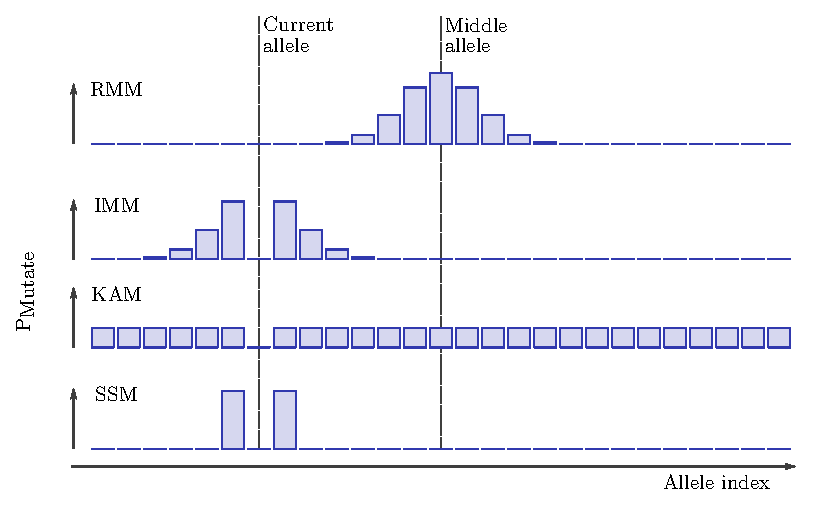
\includegraphics[width=1\textwidth]{mutation_model.pdf}
    \caption{Schematic representation of the various mutation model for a system with 27 alleles, where the reference allele is 14 and the allele from which we mutate is 7. $P_{\text{Mutate}}$ represent the probability to mutate to a given allele. Notice also that the allelic value is almost equivalent as the allelic index in quantiNemo}
    \label{fig:mutation_model}
\end{figure}

\end{description}

\subsection{neutral mutation model}
\begin{description}
\item[ntrl\_mutation\_model\index{ntrl\_mutation\_model}] \textbf{[0,1] (default: 0)}\\
In the neutral case, there is only access to two of the model, since the allelic value are not define and some of the model don't make sense. 
\begin{description}
\item[0~:~KAM] (K-Allele Model)\\
At each mutation the existing allele is randomly exchanged by another allele within the range of alleles (i.e. $[1; quanti\_all]$) not taking into account any allelic effect. The probability to mutate to any allele is the same.

\item[1~:~SSM] (Single Step Mutation)\\
In the single step mutation, the new allele depends on the current allele index. When a mutation occurs the current allele is replaced by one of its neighboring alleles. For example, if the allele with the index 12 mutates, it changes either to the allele with the index 13, or to the allele with the index 11. The boundaries are reflexive, \textit{i.e.} the allele index cannot exceed the range of alleles (i.e. $[1; ntrl\_all]$).
\end{description}
\end{description}
\section{Multiple traits}\label{sec:MultipleTraits}
QuantiNemo allows simulating multiple traits (quantitative and/or neutral) simultaneously. Each trait has its own architecture and quantitative traits may be under different selection pressures.

\begin{description}
\item[(quanti/ntrl)\_nb\_trait\index{quanti\_nb\_trait}\index{ntrl\_nb\_trait}] \textbf{[integer] (default: 1)}\\
This parameter defines the number of traits. Notice that it is possible to have ntrl traits. This has to be thought has a set of neutral loci which share common parameters, like mutation model or mutation rate. 
\end{description}

Each trait may have its own specifications, but it is also possible to specify parameters for some traits together, named grouping. If several traits are used it is possible to address a certain trait by its number. For instance to specify a parameter for the fifth trait one has to append a \textsf{"\_5"} to the parameter name. In contrast if for the fifth trait no parameter with the suffix \textsf{"\_5"} is passed quantiNemo checks if the parameter is passed for the fourth trait (suffix \textsf{"\_4"}). If this is also not the case quantiNemo checks if the parameter is passed for the third trait (suffix \textsf{"\_3"}), and so forth until a parameter is found. Note, that a parameter without a suffix is the same as the parameter with the suffix  \textsf{"\_1"}. This behavior of quantiNemo allows specifying parameters for a group of traits. Sometimes this grouping is not desired. It can be suppressed by setting 'NOT\_SET' as an argument. In this case, this parameter and all parameters inheriting this parameter will use the default argument. An example for quantitative traits may make it clearer:
\begin{lstlisting}[frame=single]
quanti_nb_trait       12
    
quanti_loci           5
quanti_loci_7         10

quanti_all_1          10
quanti_all_4          20
quanti_all_7          10
quanti_all_10         20

quanti_allelic_file_1 file_1.txt  
quanti_allelic_file_4 file_2.txt  
quanti_allelic_file_7 NOT_SET  

quanti_mutation_rate 0.0001
\end{lstlisting} 
In this example, we simulate 12 quantitative traits. Traits 1 to 3 consist of 5 loci with up to 10 alleles, traits 4 to 6 consist of 5 loci with up to 20 alleles, traits 7 to 9 consist of 10 loci with up to 10 alleles, and traits 10 to 12 consist of 10 loci with up to 20 alleles. All traits have the same mutation rate of 0.0001. Allele characteristics for traits 1 to 3 are specified in file "file\_1.txt", allele characteristics for the traits 4 to 6 in the file "file\_2.txt". Since 'NOT\_SET' is set for the parameter \textsf{ quanti\_allelic\_file\_7} all allele characteristics for traits 7 to 12 are set automatically without any file. \\

\section{Genetic map}\label{sec:geneticMap}
QuantiNemo has an underlying genetic map, which may consist of several chromosomes. This allows
explicitly positioning all types of loci on the map (quantitative trait loci (QTL) and neutral
markers). The unit of the genetic map is centi Morgans \citep[cM]{Haldane_1919}. This means that
between two loci separated by 100 cM on average a single recombination event per meiosis is expected.
The relation between centiMorgan (m) and recombination rate (r) is given as 
\[r=\frac{1-e^{-2m/100}}{2}\].

\begin{figure}[h]
    \centering
        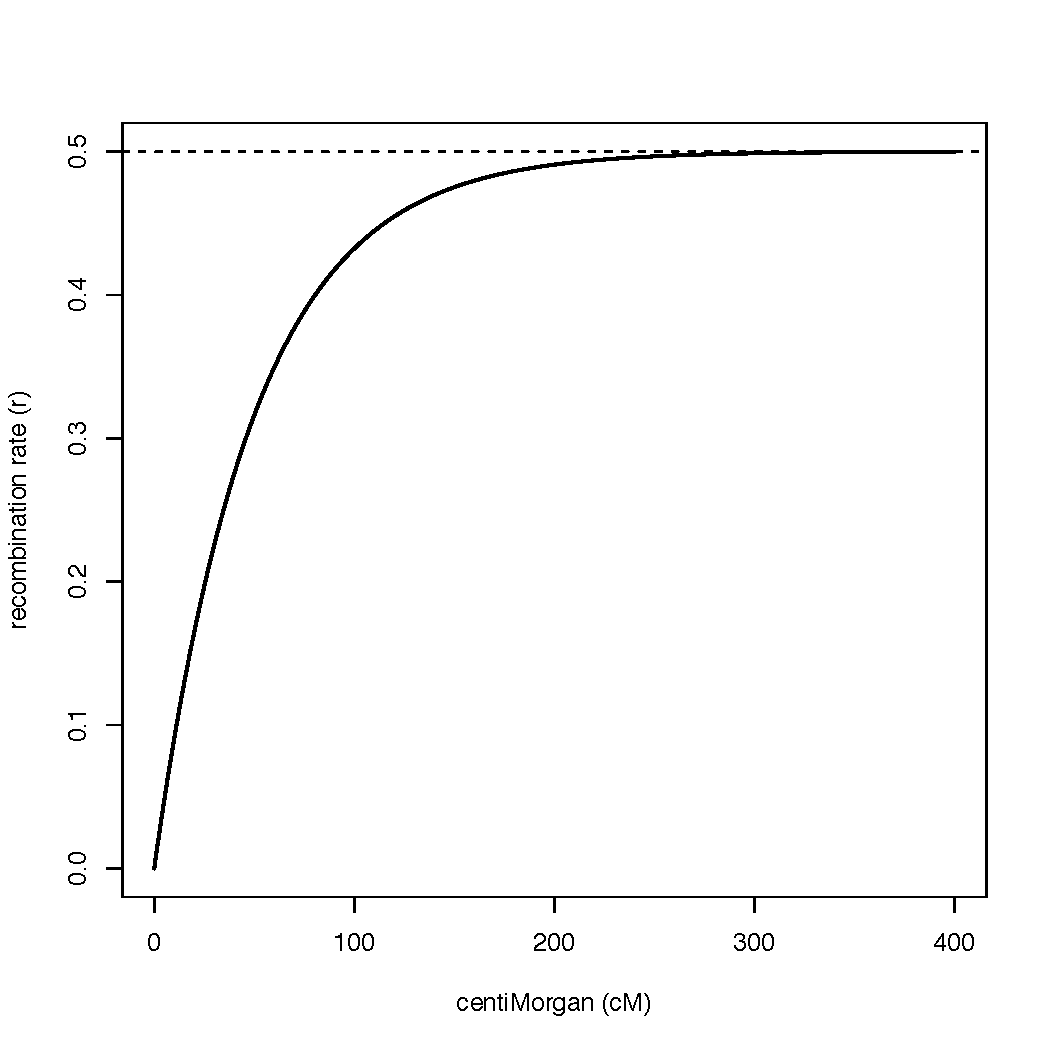
\includegraphics[width=0.70\textwidth]{cM2r.pdf}
    \label{fig:centiMorgan to recombination rate}
\end{figure}

To simulate linked loci two types of parameters have to be set: One to specify the locus positions on the genome (in cM) and one for each trait (QTL or neutral) to attribute the loci of the trait to these locus positions. If a locus of a trait is not attributed to a position then quantiNemo2 assumes that this locus is unlinked to any other locus. A genome is identical for everybody, however, sexes may differ in the rate of recombinations, e.g. hotspots of recombination, or degenerated Y-chromosome (see also parameter \textbf{sex\_ratio\_threshold}). quantiNemo2 accounts for this by allowing specifying different genetic maps (in cM) for each sex using the suffixes \textbf{\_fem} and \textbf{\_mal}. Note, that in this case, the order of loci must be identical, only distances between loci may differ.


\begin{description}
\item[genome\index{genome}]\hspace*{\fill}\\
\vspace{-9mm}
\item[genome\_fem\index{genome\_fem}]\hspace*{\fill}\\
\vspace{-9mm}
\item[genome\_mal\index{genome\_mal}]\textbf{[matrix] (default: "")}\\
These parameters allow specifying the positions of loci in centi Morgans for all traits in common.
Brackets separate different chromosomes and within a chromosome, the positions of loci are defined cumulatively, \textit{i.e.} the position of the locus is defined as the length to the start of the chromosome. Note, that
chromosomes may contain different numbers of loci. It is possible to skip chromosomes if they don't
contain loci (see section \ref{matparam}). If the genetic map is sex specific both parameters have
to be set. If hermaphrodites are simulated the parameters \textbf{genome} and \textbf{genome\_fem} are identical.
If all three parameters are set, only the sex specific parameters will be used. The genome may only
be specified in general (i.e. parameter \textbf{genome}) or for each type of trait separately (i.e.
parameters \textbf{quanti\_genome} and \textbf{ntrl\_genome}).\\


\item[(quanti/ntrl)\_genome\index{quanti\_genome}\index{ntrl\_genome}]\hspace*{\fill}\\
\vspace{-9mm}
\item[(quanti/ntrl)\_genome\_fem\index{quanti\_genome\_fem}\index{ntrl\_genome\_fem}]\hspace*{\fill}\\
\vspace{-9mm}
\item[(quanti/ntrl)\_genome\_mal\index{quanti\_genome\_mal}\index{ntrl\_genome\_mal}]\textbf{[matrix] (default: "")}\\
Similar to the parameters above these parameters allow specfiying the positions of loci in centi
Morgans. In contrast to the parameters above these parameters allow specifiying the positions for
each type of trait separately.\\

Example:
\begin{lstlisting}[frame=single]
genome { {1: 10}
         {3: 10 40 60 80 100}
         {   10 40 60 80 100} }
\end{lstlisting} 
In the example above, the genetic map consists of 11 loci located on three of at least four
chromosomes. The first chromosome contains a single locus at position 10 cM. No loci are located on
the second chromosome. The third and fourth chromosomes have 5 loci at positions 10, 40, 60, 80, and 100 cM.


\item[(quanti/ntrl)\_locus\_index\index{quanti\_locus\_index}\index{ntrl\_locus\_index}]\textbf{[matrix]
(default: "")}\\
This parameter allows assigning each locus of a trait (quanti or ntrl) to a locus position on the genome (see above). The parameter has to be set for each trait
separately and the assignment of the locus to a locus position on the genome is made based on the
index of the locus on the entier genome (starting with 1). Note, that the indexing is ignoring any
chromosomal structure. Note also, that the indexing depends on the corresponding genome, \textit{i.e.} if it
is specified in general (parameter \textbf{genome}) or trait type specific (e.g. parameter
\textbf{quanti\_genome}). Note further, that this parameter is not sex specific, since the
order of the loci is identical for both sexes.   \\

Example 1 (trait type sepcific):
\begin{lstlisting}[frame=single]
quanti_nb_trait      2
quanti_loci          3
quanti_genome        {0.1 0.2 0.3 0.4 0.5 0.6}
quanti_locus_index_1 {1 2 5}
quanti_locus_index_2 {3 4 6}
ntrl_nb_trait        2
ntrl_genome          {0.1 0.6 0.7 0.8 0.9 1.0}
ntrl_locus_index_1   {1 2 5}
ntrl_locus_index_2   {3 4 6}
\end{lstlisting} 

Example 2 (general):
\begin{lstlisting}[frame=single]
genome               {0.1 0.1 0.2 0.3 0.4 0.5 0.6 0.6 0.7 0.8 0.9 1.0}
quanti_nb_trait      2
quanti_loci          3
quanti_locus_index_1 {1 3 6}
quanti_locus_index_2 {4 5 7}
ntrl_nb_trait        2
ntrl_locus_index_1   {2 8 11}
ntrl_locus_index_2   {9 10 12}
\end{lstlisting} 

Both examples are identical, the genome is defined once for each type of trait separately (Example
1), and once in general (Example 2). In the example, we have 5 QTLs and 6 neutral markers. 
At 0.1 cM we have a QTL and a neutral marker without any recombination between them.

\item[recombination\_factor\index{recombination\_factor}]\hspace*{\fill}\\
\vspace{-9mm}
\item[recombination\_factor\_fem\index{recombination\_factor\_fem}]\hspace*{\fill}\\
\vspace{-9mm}
\item[recombination\_factor\_mal\index{recombination\_factor\_mal}]\textbf{[decimal/matrix] (temporal/default: 1)}\\
These parameters allow setting a factor for the recombination rate. This factor is then multiplied with the positions of the loci on the chromosomes allowing easily stretching or shrinking a chromosome, keeping the relation between the loci intact. These parameters allow simulating the evolution of the recombination rate. To achieve this it is possible to use the phenotype ($Z$) or the genotypic value ($G$) of a quantitative trait as recombination factor. Thereby the key character $G$ and $Z$ are followed directly by the quantitative trait index. \\

Example:
\begin{lstlisting}[frame=single]
quanti_genome        {1 4}{1 10}
recombination_factor_mal {2 0.5}
recombination_factor_fem {Z1 Z2}
\end{lstlisting}
In this example, the genome consists of two chromosomes containing each 2 loci. A recombination factor is set separately for females and males. The recombination rate for males is fixed and modifies the positions of the first chromosome by a factor of two (increasing the recombination rate among the loci) and by a factor of 0.5 for the second chromosome (reducing the recombination rate among the loci). In contrast, the recombination factor for females is variable and is given by the phenotype of the first and second quantitative trait for the first and second chromosome, respectively.


\end{description}


%%%%%%%%%%%%%%%%%%%%%%%%%%%%%%%%%%%%%%%%%%%%%%%%%%%%%%%%%%%%%%%%%%%%%%%%%%%%%%%%%%%%%%%%%%%%%%%%%%%%%%%%%%%%%%%%%%%%%%%%%%%%%%%%%%%%%%
\newpage


%%%%%%%%%%%%%%%%%%%%%%%%%%%%%%%%%%%%%%%%%%%%%%%%%%%%%%%%%%%%%%%%%%%%%%%%%%%%%%%%%

\chapter{Quantitative traits and selection}\label{chap:QuantitativeTraitsAndSelection}
\section{Introduction}
In quantiNemo,  selection is based on the fitness of individuals. It generally acts at reproduction level (for efficiency reason) but can also act at the regulation stage. 
More precisely, in a first step, the fitness of all individuals of the population are computed based on their genetic information (see below). Depending on the type of selection (soft/hard), the fitness can be further rescaled by the mean fitness of the patch/metapopulation. Then, during breeding, the parents of each individual are randomly selected proportionality to their fitness.  

Two different procedure can be used to specify the fitness of an individual. One follows the philosophy of quantitative genetic, calculating the phenotypic value of each trait and applying selection pressure to it. The other one is closer to a population genetic approach, where the fitness is specified explicitly for each genotype and locus. The two approaches can be combined, in different traits (some defined using one approach and the other using the other approach) but also in a single trait. In this case, the final fitness of the trait is the product of the fitness obtained by both procedures. 
\begin{figure}[h]
    \centering
        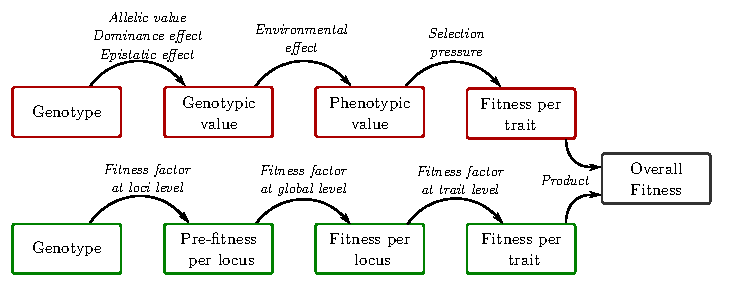
\includegraphics[width=0.80\textwidth]{selection.pdf}
    \label{fig:Selection}
\end{figure}
\subsection{Quantitative genetic approach}
\fm{I'm not sure if it's better to speak about phenotypic value or just about phenotype, which for me is more vague but maybe make more sens to new comer}
To compute the fitness of an individual, quantiNemo define a genotypic value, which is the value of a trait would have if no environmental effect plays a role (therefore, if environmental effect are set to zero, the genotypic value is equal to the phenotypic value). So first, the genotypic value for each traits is computed, from the allelic values, the dominance model and if present the epistatic value. Then, the phenotypic value is computed by adding to the genotypic value the environmental value. Overall, the phenotypic value is given by:
\begin{eqnarray}
P &=& G + E \\
G&=&\epsilon+\sum_{i=1}^{nbLoci}a_i+a_{i'}+k_{ii'}|a_{i'}-a_i| 
\end{eqnarray}
Where $P$ is the phenotypic value, $G$ the genotypic value, $E$ the environmental effect, $\epsilon$ the epistatic effect, $a_i$ and $a_{i'}$ the allelic value and $k_{ii'}$ the dominance factor. 

In a second step, the fitness of every trait is computed from its genotypic value using one of the models of selection pressure \textit{e.g.} stabilizing selection where the value of the fitness decrease when the phenotypic value is far from its optimal value. Finally, the overall fitness of each individual, which is the product of the fitness of each trait is computed.

\begin{eqnarray}
W &=& \prod_t W_t
\end{eqnarray}
where $W$ is the overall fitness and $W_t$ is the fitness of each trait. 
\subsection{Population genetic approach}
In this approach, the fitness of an individual is considered to be a product of the fitness of each of its loci. The fitness of its loci is obtained through what is called fitness factor, which directly relates the genotype of a locus to its fitness. This factor can either be specified for each genotype and each locus explicitly using the dominance file (see sub-section: \ref{sub:DominanceEffects}) or globally depending on the heterozygosity (see section \ref{sec:FitnessFactor})

In the following sections, we explain in details the parameters to define quantitative traits, the selection pressure acting and other parameters affecting the fitness and the selection. 

\section{From genotype to genotypic value }
In this section, we explain how quantiNemo compute the genotypic value from a given genotype taking into account the value of every allele, dominance effect and if it's present, epistasis. 
\subsection{Allelic effects}\label{sub:AllelicEffects}
Each allele has an allelic effect, its contribution to the genotype, which is represented by a number, the allelic value. There are two possibilities to define these effects. Either they are defined explicitly for each allele using a separate file (see parameter \textsf{quanti\_allelic\_file} in section \ref{sec:SettingsLoci}), or they can be defined by specifying the variance of the normal distribution of the genotypic value (see parameter \textsf{quanti\_allelic\_var}). If the allelic effects are defined in both ways the explicitly defined effects are used. Note, that all effects have to be defined in the same way, \textit{i.e.} explicitly or by their distribution.

\begin{description}

\item[quanti\_allelic\_var\index{quanti\_allelic\_var}] \textbf{[decimal/matrix]  (default: 1)}\\

If the allelic values are not defined explicitly using the allelic file (params. \textbf{(ntrl/quanti)\_allelic\_file}), quantiNemo will proceed as follow. The allelic values will be equally spaced between $-6 \sigma$ and $6 \sigma$, where $\sigma$ is the square root of the variance given by \textbf{quanti\_allelic\_var}. If the initial frequencies and/or the mutations frequencies toward each allele are not set by the allelic file, these frequencies will be set by a (discretized) normal distribution with a variance given by the parameter \textbf{quanti\_allelic\_var}. If dominance is purely additive, this ensures that through the population, the variance of the genotype is $2*quanti\_allelic\_var$ (the factor 2 comes from the diploid character of individuals).

Note that if the number of alleles is small (smaller than 6), the allelic values will be spaced between $-(l-1)\sigma$ and $(l-1)\sigma$ instead of  $-6 \sigma$ and $6 \sigma$  where $l$ is the number of alleles. So for example, for a bi-allelic system, we would have two allelic values at $-\sigma$ and $\sigma$.
\end{description} 

\subsection{Dominance effects}
\label{sub:DominanceEffects}
By default alleles are considered to be purely additive. Dominance effects can be defined in different ways. Either the dominance effect of specific pairs of alleles are defined explicitly using a separate file (parameter \textsf{quanti\_dominance\_file}), or by defining the normal distribution from where the dominance effects are randomly drawn (see parameters \textsf{quanti\_dominance\_mean} and \textsf{quanti\_dominance\_var}). An explicitly defined dominance effect has precedence over the general settings. By default, the parameters \textsf{quanti\_dominance\_mean} and \textsf{quanti\_dominance\_var} are set to zero resulting in a purely additive genotypic value of a locus. There are also two methods to define dominance:
\begin{description}
\item [quanti\_dominance\_model\index{quanti\_dominance\_model}] \textbf{[0,1] (default: 0)} \\
This parameter allows to choose among two models to define dominance
effects.
\begin{description}
\item [0 : method k.] $G_{i} = a_{i} + a_{i'} + k_{ii'}|a_{i} - a_{i'}|$
\item [1 : method h.] $G_{i} = 2[(1 - h_{ii'})a_{i} + h_{ii'}a_{i'}]$
\end{description}
Where $G_{i}$ is the genotypic value of locus $i$, $a_{i}$ and $a_{i'}$ are the effects of the two alleles at locus $i$, whereas the effect of $a_{i}$ is smaller than the effect of $a_{i'}$. $k_{ii'}$ and $h_{ii'}$ are the dominance values between allele $i$ and $i'$ for method 1 and method 2, respectively. $k$ and $h$ can have the following effects: \\

\begin{tabular}{lll}
\hline
Effect                                      & method k  & method h \\
\hline
overdominance                      & $k< -1$     & $h< 0$     \\
smaller allele $a_{i}$ is dominant &$ k = -1$        &$ h = 0 $       \\
purely additive         & $k = 0$         &$h =  0.5$      \\
larger allele $a_{i'}$ is dominant & $k = 1$         & $ h = 1$        \\
underdominance                     & $k > 1$     & $h > 1$    \\
\hline
\end{tabular}

\item[quanti\_dominance\_file\index{quanti\_dominance\_file}] \textbf{[string] (default: "")}\\
This parameter allows to pass the name of a file containing the dominance effects and/or the fitness factor (see section \ref{sec:FitnessFactor}). The information can be set globally for all loci, if they have the same specifications, or for each locus separately. For all not specified allele pairs other settings or the default values are applied. The dominance file has a similar format as the allelic file:

\begin{lstlisting}[frame=single]
#Dominance file 
####################
[FILE_INFO]{
  col_locus          1
  col_allele1        2
  col_allele2        3
  col_dominance      4
  col_fitness_factor 5
}

#locus  allele1  allele2  dominanc fitness
1       1        1        99999    1
1       1        2        0.298    1
1       1        3        0.435    1
1       1        4        0.224    1
1       2        2        99999    1
1       2        3        0.104    1
1       2        4        0.974    1
1       3        3        99999    1
1       3        4        0.808    1
1       4        4        99999    0
\end{lstlisting}

The file has to start with a file information box \textsf{[FILE\_INFO]}\{...\}. 
This box contains information about the structure of the following table and thus allowing flexibility in the format of the table. For example, the order of the columns in the table may vary, or some columns may be ignored. The file information box starts with the keyword \textsf{[FILE\_INFO]}. This keyword is followed by brackets "\{...\}" within which the user has to specify the contents of the columns to be considered by quantiNemo. Each column is specified by a pair consisting of a keyword (e.g. \textsf{col\_locus} followed by the column number (the ordering starts with 1). Each column definition has to be on a new line. The following column keywords are available:
\begin{description}
\item [col\_locus] This keyword specifies the column containing the locus index. If this column is not declared in the file information box, quantiNemo will use the same settings (dominance effect and/or fitness factor) for all loci.
\item [col\_allele1] This keyword specifies the column containing the index of the allele with the smaller allelic effect. This column is mandatory. The index of the allele goes from 1 to \textsf{quanti\_all}.
\item [col\_allele2] This keyword specifies the column containing the index of the allele with the larger allelic effect. This column is mandatory. The index of the allele goes from 1 to \textsf{quanti\_all}.
\item [col\_dominance] This keyword specifies the column containing the dominance effects. For any pair of alleles for which the dominance effect is not specified a dominance effect will be drawn from the normal distribution defined by the parameters  \textsf{quanti\_dominance\_mean} and \textsf{quanti\_dominance\_var}.
\item [col\_fitness\_factor] This keyword specifies the column containing the fitness factors (see section \ref{sec:FitnessFactor} for more informations). For any pair of alleles for which the fitness factor is not specified explicitly the fitness factor will be zero or given by the parameters \textsf{quanti\_sel\_fitness\_factor} or \textsf{quanti\_fitness\_factor\_homozygote} if they are defined.
\end{description} 
Note, that as in all input files for quantiNemo it is possible to add comments (also in the file information box) using the hash character: '\#' or '\#/ ...any text... /\#'. If you define explicitly the dominance effect and the fitness factor, but for a given pair of alleles you want only to define one of the parameters you may use the number \textit{99999} as placeholders. quantiNemo will treat this number as not set. In the above example, this has been used to show that a dominance effect for a monomorphic locus is not valid (However a fitness factor may be set for a monomorphic locus). Please note that in this special case (monomorphic locus) one could have set any number as placeholders for the dominance effect since the value would never be used.   

\item[quanti\_dominance\_mean\index{quanti\_dominance\_mean}] \textbf{[decimal] (default: 0)} \\
This parameter allows specifying the mean of the normal distribution from where the dominance effects are randomly drawn. Note that $a_{1}$ has the smaller allelic effect than $a_{2}$. This parameter is only taken into account if the dominance effects are not defined explicitly by the dominance file.

\item[quanti\_dominance\_var\index{quanti\_dominance\_var}] \textbf{[decimal] (default: 0)} \\
This parameter allows specifying the variance of the normal distribution from where the dominance effects are randomly drawn. This parameter is taken into account only if the dominance effects are not defined explicitly by the dominance file.
\end{description} 


\subsection{Epistatic effects}
\label{sub:EpistaticEffects}
It is possible to simulate epistatic effects between alleles at different loci. The following equation is used to compute the genotype:

\[G_{11'22'...kk'...}=\epsilon_{11'22'...kk'...}+\sum_{i=1}^{nbLoci}G_{i} \]

Where $G_{11'22'...kk'...}$ is the genotypic value of genotype ${11'22'...kk'...}$ ($1$ and $1'$ are the alleles of locus 1, $2$ and $2'$ the alleles of locus 2, ...), $G_{i}$ is the genotypic effect of locus $i$ (additive and dominance effects), and $\epsilon_{11'22'...kk'...}$ is the epistatic effect of genotype $11'22'...kk'...$ (unique for each multilocus genotype). There are two possibilities to define epistatic effects. Either they are defined explicitly for each genotype using a separate file (see parameter \textsf{quanti\_epistatic\_file}), or by defining the variance of the normal distribution from where the epistatic effects are randomly drawn (see parameter \textsf{quanti\_epistatic\_var}). Using the parameter \textsf{quanti\_epistatic\_file} it is also possible to define the genotypic effects directly. If the epistatic effects are defined in both ways the explicitly defined effects are used. Note, that all effects have to be defined in the same way, \textit{i.e.} explicitly or by their distribution. By default, the parameter \textsf{quanti\_epistatic\_var} is set to zero resulting in simulations without any epistatic effects.

\begin{description}
\item[quanti\_epistatic\_file\index{quanti\_epistatic\_file}] \textbf{[string] (default: "")}\\
This parameter allows to pass the name of a file containing the epistatic effects and/or the fitness factor (see section \ref{sec:FitnessFactor}). The number of defined genotypes has to be in line with the parameters \textsf{quanti\_loci} and \textsf{quanti\_all} if epistatic or genotypic values are passed. If only fitness factors are defined it is enough to list the desired genotypes with their fitness factors. In this case all not specified genotypes have a fitness factor of 1. The epistatic file has a similar format as the allelic file:

\begin{lstlisting}[frame=single]
#Epistatic file 
####################
[FILE_INFO]{
  col_genotype 1
  col_epistatic_value 2
  # col_genotypic_value 3
  col_fitness_factor 4
}

#genotype       epistaticVal  genotypicVal  fitness
{0101 0101}     0.242984      1.87009       1    
{0101 0102}     0.580787      0.834811      99999   
...
{5050 5048}     0.264001      1.24981       0
{5050 5049}     0.118982      -0.55701      1
{5050 5050}     0.071359      -2.26644      1
\end{lstlisting}

The file has to start with a file information box \textsf{[FILE\_INFO]}\{...\}. 
This box contains informations about the structure of the following table and thus allowing flexibility in the format of the table. For example the order of the columns in the table may vary, or some columns may be ignored. The file information box starts with the key word \textsf{[FILE\_INFO]}. This key word is followed by brackets "\{...\}" within which the user has to specify the contents of the columns to be considered by quantiNemo. Each column is specified by a pair consisting of a key word (e.g. \textsf{col\_locus} followed by the column number (the ordering starts with 1). Each column definition has to be on a new line. The following column keywords are available:
\begin{description}
\item [col\_genotype] This keyword specifies the column containing the genotype. This column is mandatory. The genotype is enclosed by brackets "\{...\}" and the genotype itself has to be in the FSTAT format \citep{Goudet_1995}. The two alleles of a locus are written consecutively without any space. For all alleles the same number of digits are needed. Two different loci are separated by a space. The above example consists of two loci, each with 50 alleles. Each allele is written using two digits. 
\item [col\_epistatic\_value] This keyword specifies the column containing the epistatic effects. If this column is set the epistatic effect is added to the genotypic effect computed as described above.
\item [col\_genotypic\_value] This keyword specifies the column containing directly the genotypic effects. If this column is set, the genotypic effect of each genotype is set directly without taking into account allelic, dominance, and/or epistatic effects. If both keywords \textsf{col\_epistatic\_value} and \textsf{col\_genotypic\_value} are specified in the information box, only the column \textsf{col\_genotypic\_value} is considered. 
\item [col\_fitness\_factor] This keyword specifies the column containing the fitness factors. For more informations on the fitness factor see please section \ref{sec:FitnessFactor}. For each genotype the fitness factor is not specified explicitly the fitness factor will be taken either from dominance file (parameter \textsf{quanti\_dominance\_file}) or from the global parameters \textsf{quanti\_sel\_fitness\_factor} and \textsf{quanti\_fitness\_factor\_homozygote}. If a genotype is listed to define the genotypic or epistatic value, but you don't want to define explicitly the fitness factor for this genotype you may use the number \textit{99999} as placeholder. quantiNemo will treat this number as not set. In the above example this has been used to show that a fitness factor for a given genotype is not set.
\end{description} 
Note, that as in all input files for quantiNemo it is possible to add comments (also in the file information box) using the hash character: '\#' or '\#/ ...any text... /\#'.

\item[quanti\_epistatic\_var\index{quanti\_epistatic\_var}] \textbf{[decimal] (default: 0)} \\
This parameter allows specifying the variance of the normal distribution from where the epistatic effects are drawn randomly. The normal distribution is centered around 0. This parameter is only taken into account if the epistatic effects are not defined explicitly by the epistatic file.
\end{description}
\section{Environmental effect}

The phenotype is given by the sum of the genotypic value and the environmental contribution. There are several possibilities to set the contribution of the environment to the phenotype globally or for each patch separately. By default (without any specification of the following parameters) the environment has no effect on the phenotype of the quantitative trait. Either the contribution of the environment to the phenotype is defined directly by the variance of the environmental effect (model 0), by the narrow-sense heritability $h^{2}$ (model 1 and 2), or by the broad-sense heritability $H^{2}$ (model 3 and 4). The heritability is later translated into a corresponding environmental variance $V_{E}$: 

\[h^{2}: \qquad V_{E} = \frac{1-h^{2}}{h^{2}}*V_{A}\]
\[H^{2}: \qquad V_{E} = \frac{1-H^{2}}{H^{2}}*V_{G}\]

Where $V_{A}$ is the additive genetic variance computed following \citep[p85-87]{Lynch_1998}, and $V_{G}$ the genetic variance.  
\begin{description}
\item[quanti\_environmental\_model\index{quanti\_environmental\_model}] \textbf{[0-4] (default: 0)}\\
This parameter specifies how the environmental variance is defined. The following models are available:
\begin{description}
\item [0~:~set $V_{E}$ directly.] The variance of the environment is set directly by the parameter \textsf{quanti\_heritability}, which is in this case not the heritability, but the environmental variance.
\item [1~:~$V_{E}$ defined by the narrow-sense heritability ($V_{E}$ constant).] The variance of the environment ($V_{E}$) is set at the beginning of a simulation (generation 1) and is based on the narrow-sense heritability ($h^{2}$, parameter \textsf{quanti\_heritability}) and the additive genetic variance ($V_{A}$ at generation 1). Note, that in this case, the environmental variance remains constant over time, but not the heritability.
\item [2~:~$V_{E}$ defined by the narrow-sense heritability ($h^{2}$ constant).] This is the same as model 1, but the environmental variance is readjusted at each generation. Thus the narrow-sense heritability remains constant over time, but not the environmental variance. 
\item [3~:~$V_{E}$ defined by the broad-sense heritability ($V_{E}$ constant).] The variance of the environment ($V_{E}$) is set at the beginning of a simulation (generation 1) and is based on the broad-sense heritability ($H^{2}$, parameter \textsf{quanti\_heritability}) and the genetic variance ($V_{G}$ at generation 1). Note, that in this case, the environmental variance remains constant over time, but not the heritability.
\item [4~:~$V_{E}$ defined by the broad-sense heritability ($H^{2}$ constant).] This is the same as model 3, but the environmental variance is readjusted at each generation. Thus the broad-sense heritability remains constant over time, but not the environmental variance. 
\end{description}

\item[quanti\_heritability\index{quanti\_heritability}] \textbf{[decimal/matrix] (default: 0)}\\
This parameter has different meaning depending on the environmental model chosen (parameter \linebreak\textsf{quanti\_environmental\_model}): If $V_{E}$ is directly set (model 0) this parameter is the environmental variance. 

For the environmental model 1 and 2 this parameter is the narrow-sense heritability ($h^{2}$):
    \[h^{2} = V_{A}/V_{P}\]
    
For the environmental model 3 and 4 this parameter is the broad-sense heritability ($H^{2}$):
    \[H^{2} = V_{G}/V_{P}\]
Note, that a heritability (narrow and broad sense) of 0 (no genetic component) makes no sense for models 1 to 4 in this simulation framework. Therefore a value of 0 is not accepted by quantiNemo for models 1 to 4, resulting in an error message. If the parameter \textsf{quanti\_environmental\_model} is set to 0 the parameter \textsf{quanti\_heritability} is no longer the heritability, but the environmental variance directly, and can be set to 0 (default). Using a matrix as argument it is possible to set the environmental variance, respectively heritability for each patch separately.

\item [quanti\_environmental\_proportion\index{quanti\_environmental\_proportion}] \textbf{[decimal] (default: 1)}\\
This parameter specifies which environment affects the phenotype of the quantitative trait: the natal or the current (at the adult stage) environment? The argument specifies the relative weight of the current patch effect on the phenotype: if the value is 1 (default value) only the environmental variance of the current patch affects the phenotype while if the value is 0 only the environmental variance of the natal patch affects the phenotype.

\item [quanti\_va\_model\index{quanti\_va\_model}] \textbf{[0-2] (default: 0)}\\
This parameter specifies how the additive genetic variance ($V_{A}$) of a quantitative trait is computed. The additive genetic variance of a trait is used in several statistics. For instance it is used to set the environmental variance of the patches if this variance is specified by the narrow-sense heritability ($h2$, parameter \textsf{quanti\_environmental\_model} set to 2 or 3, see also parameter \textsf{quanti\_heritability}), the additive genetic variance may also be directly output as summary statistic (stat option $q.varA$), or indirectly in the population differentiation measurement $Q_{ST}$ (stat option $q.qst$, $q.qst.f$, $q.qst_pair$, and $q.qst.f_pair$).
The additive genetic variance ($V_{A}$) is computed following \citet[p85-87]{Lynch_1998}. For a quantitative trait determined by a single locus this is:

\[ V_{A} = 2\sum_{i=1}^{nbAllele}p_{i}\alpha_{i}\alpha_{i}^{*} \]

Where $p_{i}$ is the allele frequency of allele $i$, $\alpha_{i}$ is the additive effect of allele $i$, and $\alpha_{i}^{*}$ is the average excess of allele $i$. Note, that we show here the computation for a single locus for simplicity reasons. In quantiNemo, a full version for traits determined by multiple loci is implemented. However, the implementation does not take into account linkage between loci, thus the additive genetic variance is underestimated when loci are linked.

\begin{description}
\item [0~:~for any case.] If this model is chosen the additive effect ($\alpha_{i}$) and the average excess ($\alpha_{i}^{*}$) are computed. While the average excess is simple to compute, the computation of the additive effect requires a time consuming least-square regression. This formula is valid for any mating system, but its computation is rather slow. 

Note, that the least-square regression has not always a solution thus the additive effects $\alpha$, are not always computable. In this case, the locus in question is skipped from the analysis and a warning is returned:
\begin{lstlisting}[frame=single]
***WARNING*** Va could not be correctly estimated (1. time
 at generation 20, see manual parameter 'quanti_va_model')
\end{lstlisting}

This warning is returned the first 10 times the problem occurs and then every hundredth time. It is up to the user to decide whether the problem occurs too often or if these "missing points" are acceptable. If the environmental variance is set by the narrow-sense heritability (parameter \textsf{quanti\_environmental\_model} set to 1 or 2) and the additive genetic variance cannot be computed quantiNemo uses the additive genetic variance computed using the algorithm for random matings (this parameter set to 1). Note, that  

 
\item [1~:~limited to random mating.] In case of random mating, the additive effect ($\alpha_{i}$) and the average excess ($\alpha_{i}^{*}$) are identical. Therefore the time consuming computation of the additive effect can be omitted. Note, that even when the mating system is set to random mating (parameter \textsf{mating\_system} set to 0 or 2) mating is not randomly if selection acts, as the choice of the parents depends on their fitnesses. It's up to the user to decide whether this quick way to compute the additive genetic variance is appropriate or not.  

\item [1~:~$V_{A} = V_{G}$.] This model assumes that the additive genetic variance $V_{A}$ is identical or may be approximated by the genetic variance $V_{G}$. 
\end{description}
\end{description}

\section{Selection pressure}\label{sec:SelectionPressure}
Each quantitative trait is under a specific selection pressure. The type of selection may vary among quantitative traits, but not among patches and sexes. However, the strength, direction, etc,  of selection can change among patches, sex and time. This flexibility allows for example to simulate a dynamic environment such as for global warming or variation in the altitude between patches. To specify the selection pressure individually for quantitative traits and patches, matrices may be used. 
\subsection{Selection models}\label{sub:SelectionModels}
Selection pressures have to be specified either for each sex separately (parameters with the suffix "\_fem" for females and "\_mal" for males), or for both sexes together (parameters without a suffix). In the first case both sex specific parameters have to be set if two sexes are simulated. In the latter case, the selection pressure of females and males are assumed to be identical.

\begin{description}
\item[quanti\_selection\_model\index{quanti\_selection\_model}]\textbf{[0-4] (default: 0)}\\
This parameter allows defining the selection model for each quantitative trait. By default no selection acts on a quantitative trait. 
\begin{description}

\item [0~:~neutral quantitative trait.] \textbf{}\\
The phenotype of this trait does not feel any selective pressure. Selection might act only ifs fitness factor is set, otherwise, it behaves as a neutral trait :
\[ W_{t} = 1\]
 
\item [1~:~stabilizing selection] \textbf{}\\
Stabilizing selection acts on the quantitative trait. The fitness $W$ of quantitative trait $t$ is
computed using the following standard Gaussian function for stabilizing selection:

\[W_{t} = e^{\left(-\frac{\left(P-Z_{Opt}\right)^2}{2\omega^{2}}\right)} \]

$Z_{Opt}$ is the selection optimum of the current trait and patch, $P$ is the phenotypic value of the individual, and $\omega$ is the intensity of the selection. See subsection \ref{sub:StabilizingSelection} for more details.  

\item [2~:~directional selection.] \textbf{}\\
Directional selection acts on the quantitative trait. A generalized logistic curve \citep{Richards_1959} is implemented in quantiNemo to characterize the directional selection pressure:

    \[ W_{t} = \left(1+s*e^{r(P_{r_{Max}}-P)}\right)^{-1/s}\]

Where $r$ is the growth rate, $P_{r_{Max}}$ is the phenotype with the maximal slope, and $s$ defines the symmetry of the slope. See subsection \ref{sub:DirectionalSelection} for more details.  

\item [3~:~fitness landscape.] \textbf{}\\
The selection pressure is defined by a fitness landscape. The fitness value of any phenotype may be specified. The fitness value of a phenotype within the specified range of phenotypes is linearly interpolated, Phenotype outside the range of specified phenotypes will result in the fitness value of the smallest phenotype, respectively in the fitness value of the largest phenotype. See subsection \ref{sub:FitnessLandscape} for more details.  
 
\item [4~:~selection coefficient.] \textbf{}\\
The selection pressure of a bi-allelic locus is defined by a selection coefficient $s$ and a dominance factor $h$. In this simplified, but widespread model, the genotype is directly mapped to a fitness. Note that for this type of selection a trait may only contain a single bi-allelic locus, without explicitly specified allelic effects.  See subsection \ref{sub:SelectionCoefficient} for more details.   \\

\begin{tabular}{ccc}
 \hline            
Genotype & Fitness & Fitness extended \\
\hline
AA & 1             & F      \\
Aa & 1 - hs & F - hs \\
aa & 1 - s     & F - s  \\
\hline
\end{tabular}


\end{description}
\end{description}



\subsection{Stabilizing selection}\label{sub:StabilizingSelection}
Stabilizing selection act on the phenotype ($P$) of quantitative traits. The selection pressure is defined by the parameters \textsf{quanti\_stab\_sel\_optima} ($Z_{Opt}$) and \textsf{quanti\_stab\_sel\_intensity} ($\omega$). The fitness (\textit{W}) of a quantitative trait is computed using the following standard Gaussian function for stabilizing selection: 

\[W = e^{\left(-\frac{\left(P-Z_{Opt}\right)^2}{2\omega^{2}}\right)} \]

\begin{figure}[h]
    \centering
        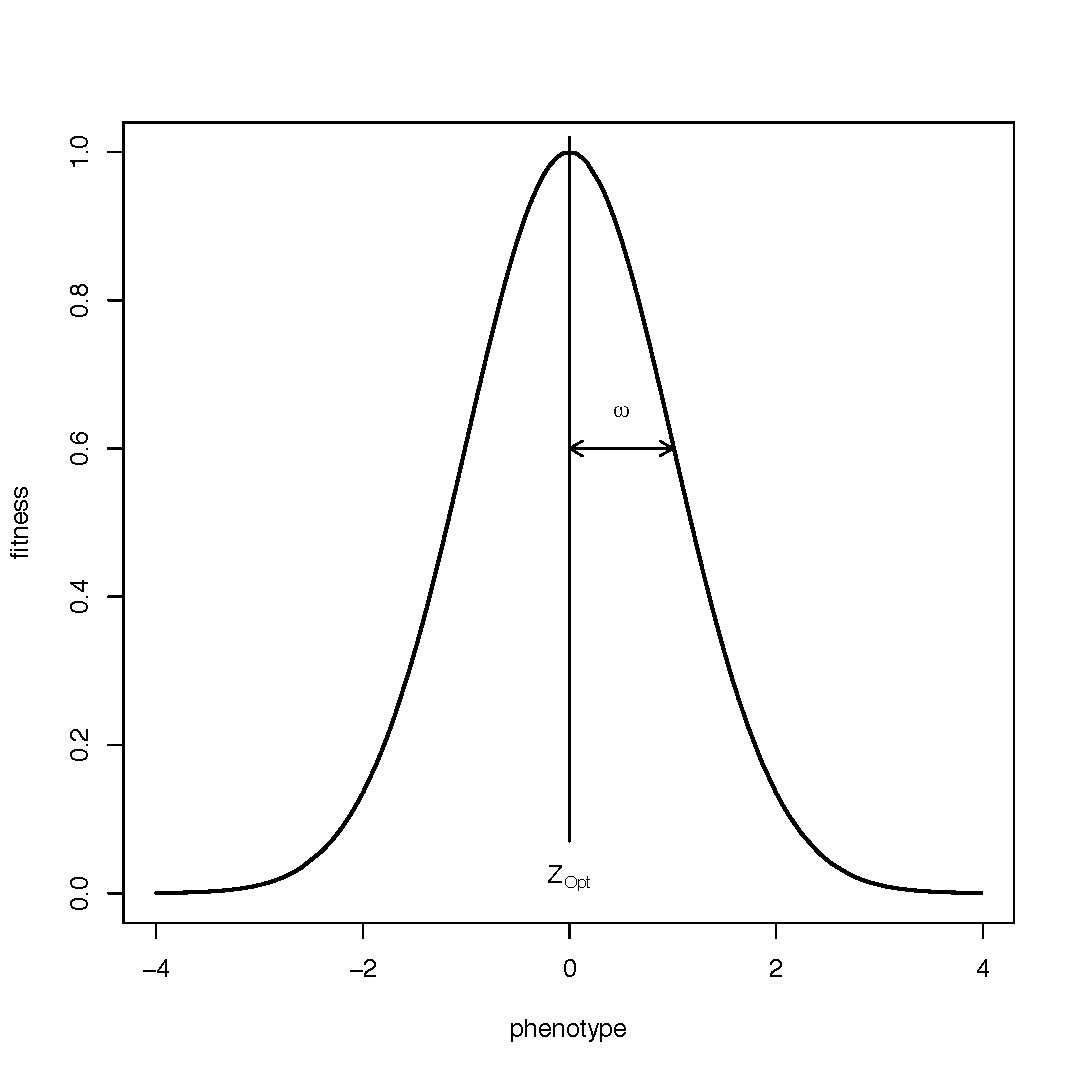
\includegraphics[width=0.70\textwidth]{stabilizing-selection.pdf}
    \label{fig:stabilizing-selection}
\end{figure}



\begin{description}

\item[quanti\_stab\_sel\_optima\index{quanti\_stab\_sel\_optima}]\hspace*{\fill}\\
\vspace{-9mm}
\item[quanti\_stab\_sel\_optima\_fem\index{quanti\_stab\_sel\_optima\_fem}]\hspace*{\fill}\\
\vspace{-9mm}
\item[quanti\_stab\_sel\_optima\_mal\index{quanti\_stab\_sel\_optima\_mal}]\textbf{[decimal/matrix] (temporal/default: 0)}\\
These parameters allow to set the selection optimum $z_{Opt}$ for each patch for a given quantitative trait.

\item[quanti\_stab\_sel\_intensity\index{quanti\_stab\_sel\_intensity}]\hspace*{\fill}\\
\vspace{-9mm}
\item[quanti\_stab\_sel\_intensity\_fem\index{quanti\_stab\_sel\_intensity\_fem}]\hspace*{\fill}\\
\vspace{-9mm}
\item[quanti\_stab\_sel\_intensity\_mal\index{quanti\_stab\_sel\_intensity\_mal}]\textbf{[decimal/matrix] (temporal/default: 1)}\\
These parameters allow to set the selection intensity $\omega$ for each patch for a given quantitative trait. Contraintuitively a small value results in a strong selection pressure, whereas a large value results in a weak selection pressure.

%Note that this parameter starts with patch instead of quanti. The quanti version was never implemented (and does not work). The patch_ version seems to work even if the selection is done at the "quantitative level". 
{\item[patch\_stab\_sel\_optima\_var\index{patch\_stab\_sel\_optima\_var}]\textbf{[decimal/matrix] (temporal/default: 0)}\\
This parameter specifies the variance of the normal distribution by which the selection optimum varies between generations (e.g. annual fluctuations of the mean temperature). By default the local selection optimum does not vary.}

{\item[patch\_stab\_sel\_intensity\_var\index{patch\_stab\_sel\_intensity\_var}]\textbf{[decimal/matrix] (temporal/default: 0)}\\
This parameter specifies the variance of the normal distribution by which the selection intensity varies at each generation (e.g. annual fluctuations of the mean temperature). By default the local selection intensity does not vary.}
\end{description}

\paragraph{Example}\hspace*{\fill}
\begin{lstlisting}[frame=single]
patch_number             2
quanti_nb_trait          3
quanti_stab_sel_optima_1 {-0.1  0.1}                            
quanti_stab_sel_optima_2 { 0.2  0.2}
quanti_stab_sel_optima_3 {-0.3  0.3}    
quanti_stab_sel_intensity 1                                                    
\end{lstlisting}
In this example the environment consist of two patches with varying selection pressures. Three quantitative traits are simulated. The first trait has a selection optimum at -0.1 in patch 1 and at 0.1 in patch 2. The selection optimum of the second trait is the same in both patches (0.2). The third trait has an optimum at -0.3 in patch 1 and at 0.3 in patch 2. The intensity of the selection is identical for all three traits and in both patches.    

\subsection{Directional selection}\label{sub:DirectionalSelection}
Directional selection may act on quantitative traits. The fitness (\textit{W}) of a quantitative trait is computed using the following generalized logistic function \citep{Richards_1959}: 

        \[ W = min + \frac{max-min}{(1+s*e^{r(P_{r_{Max}}-P)})^{1/s}} \] 

\begin{figure}[h]
    \centering
        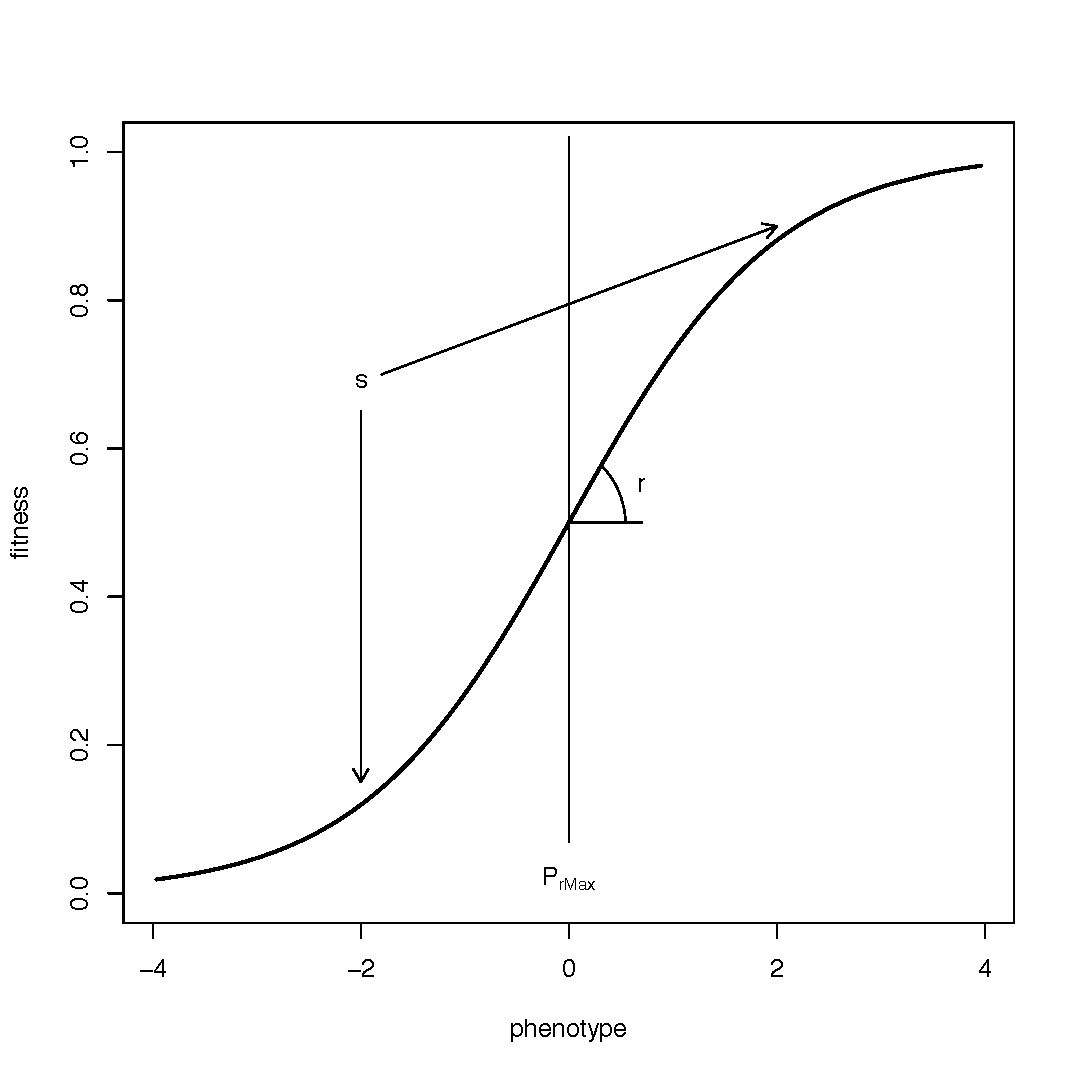
\includegraphics[width=0.70\textwidth]{directional-selection.pdf}
    \label{fig:directional-selection}
\end{figure}


Where $min$ is the lower asymptote (parameter \textsf{quanti\_dir\_sel\_min}), $max$ is the upper asymptote (parameter \textsf{quanti\_dir\_sel\_max}), $r$ is the growth rate (parameter \textsf{quanti\_dir\_sel\_growth\_rate}), $P_{r_{Max}}$ is the phenotype with the maximal slope (parameter \textsf{quanti\_dir\_sel\_max\_growth}), and $s$ defines the symmetry of the curve (parameter \textsf{quanti\_dir\_sel\_symmetry}; the curve is symmetric by default (value 1)).


\begin{description}

\item[quanti\_dir\_sel\_min\index{quanti\_dir\_sel\_min}]\hspace*{\fill}\\
\vspace{-9mm}
\item[quanti\_dir\_sel\_min\_fem\index{quanti\_dir\_sel\_min\_fem}]\hspace*{\fill}\\
\vspace{-9mm}
\item[quanti\_dir\_sel\_min\_mal\index{quanti\_dir\_sel\_min\_mal}]\textbf{[decimal/matrix] (temporal/default: 0)}\\
These parameters allow to set the lower asymptote of the selection curve for each patch for a given quantitative trait.

\item[quanti\_dir\_sel\_max\index{quanti\_dir\_sel\_max}]\hspace*{\fill}\\
\vspace{-9mm}
\item[quanti\_dir\_sel\_max\_fem\index{quanti\_dir\_sel\_max\_fem}]\hspace*{\fill}\\
\vspace{-9mm}
\item[quanti\_dir\_sel\_max\_mal\index{quanti\_dir\_sel\_max\_mal}]\textbf{[decimal/matrix] (temporal/default: 1)}\\
These parameters allow to set the upper asymptote of the selection curve for each patch for a given quantitative trait.

\item[quanti\_dir\_sel\_growth\_rate\index{quanti\_dir\_sel\_growth\_rate}]\hspace*{\fill}\\
\vspace{-9mm}
\item[quanti\_dir\_sel\_growth\_rate\_fem\index{quanti\_dir\_sel\_growth\_rate\_fem}]\hspace*{\fill}\\
\vspace{-9mm}
\item[quanti\_dir\_sel\_growth\_rate\_mal\index{quanti\_dir\_sel\_growth\_rate\_mal}]\textbf{[decimal/matrix] (temporal/default: 1)}\\
These parameters allow to set the slope of the selection curve for each patch for a given quantitative trait. If the argument is positive larger phenotypes have a higher fitness, while if negative smaller phenotypes have a higher fitness. 

\item[quanti\_dir\_sel\_max\_growth\index{quanti\_dir\_sel\_max\_growth}]\hspace*{\fill}\\
\vspace{-9mm}
\item[quanti\_dir\_sel\_max\_growth\_fem\index{quanti\_dir\_sel\_max\_growth\_fem}]\hspace*{\fill}\\
\vspace{-9mm}
\item[quanti\_dir\_sel\_max\_growth\_mal\index{quanti\_dir\_sel\_max\_growth\_mal}]\textbf{[decimal/matrix] (temporal/default: 0)}\\
These parameters allow to set the phenotype with the maximal growth.

\item[quanti\_dir\_sel\_symmetry\index{quanti\_dir\_sel\_symmetry}]\hspace*{\fill}\\
\vspace{-9mm}
\item[quanti\_dir\_sel\_symmetry\_fem\index{quanti\_dir\_sel\_symmetry\_fem}]\hspace*{\fill}\\
\vspace{-9mm}
\item[quanti\_dir\_sel\_symmetry\_mal\index{quanti\_dir\_sel\_symmetry\_mal}]\textbf{[decimal/matrix] (temporal/default: 1)}\\
These parameters allow to set the symmetry of the curve. The default value of 1 results in a symmetric slope. 

{\item[patch\_dir\_sel\_min\_var\index{patch\_dir\_sel\_min\_var}]\textbf{[decimal/matrix] (temporal/default: 0)}\\
This parameter specifies the variance of the normal distribution by which the lower asymptote of the selection curve varies at each generation (e.g. annual fluctuations of the mean temperature). By default the lower asymptote of the selection curve does not vary.}

{\item[patch\_dir\_sel\_max\_var\index{patch\_dir\_sel\_max\_var}]\textbf{[decimal/matrix] (temporal/default: 0)}\\
This parameter specifies the variance of the normal distribution by which the upper asymptote of the selection curve varies at each generation (e.g. annual fluctuations of the mean temperature). By default the upper asymptote of the selection curve does not vary.}

{\item[patch\_dir\_sel\_growth\_rate\_var\index{patch\_dir\_sel\_growth\_rate\_var}]\textbf{[decimal/matrix] (temporal/default: 0)}\\
This parameter specifies the variance of the normal distribution by which the selection slope varies at each generation (e.g. annual fluctuations of the mean temperature). By default the local selection slope does not vary.}

{\item[patch\_dir\_sel\_max\_growth\_var\index{patch\_dir\_sel\_max\_growth\_var}]\textbf{[decimal/matrix] (temporal/default: 0)}\\
This parameter specifies the variance of the normal distribution by which the phenotype with maximal growth varies at each generation (e.g. annual fluctuations of the mean temperature). By default the local phenotype with maximal growth does not vary.}

{\item[patch\_dir\_sel\_symmetry\_var\index{patch\_dir\_sel\_symmetry\_var}]\textbf{[decimal/matrix] (temporal/default: 0)}\\
This parameter specifies the variance of the normal distribution by which the symmetry of the curve varies at each generation (e.g. annual fluctuations of the mean temperature). By default the symmetry of the slope does not vary.}
\end{description}

\paragraph{Example}\hspace*{\fill}
\begin{lstlisting}[frame=single]
quanti_dir_sel_growth_rate 1    
quanti_dir_sel_max_growth  0    
quanti_dir_sel_symmetry    1    
\end{lstlisting}
In this example the selection pressure for all patches and quantitative traits are identical and set to the default values. The specified directional selection pressure favours larger phenotypes (parameter \textsf{quanti\_dir\_sel\_growth\_rate} is positive). This means that individuals with larger phenotypes have on average higher fitnesses and thus higher reproductive successes.

\subsection{Fitness landscape}\label{sub:FitnessLandscape}
Specifying a fitness landscape allows defining any selection pressure for a given quantitative trait. More precisely, it allows to associate to any value of the trait (\textit{i.e.} phenotypic value) a given fitness. The phenotypic values (parameter \textsf{quanti\_phenotype\_landscape}) and fitness values (parameter \textsf{quanti\_fitness\_landscape}) are separately passed to quantiNemo as two vectors. The fitness value of any phenotype within the specified range of phenotypes is linearly interpolated and if the phenotype lies outside of the specified range of phenotypes the resulting fitness value will result in the fitness value of the smallest and largest phenotype, respectively. By default, all phenotypes will result in a fitness of 1. 

\begin{figure}[h]
    \centering
        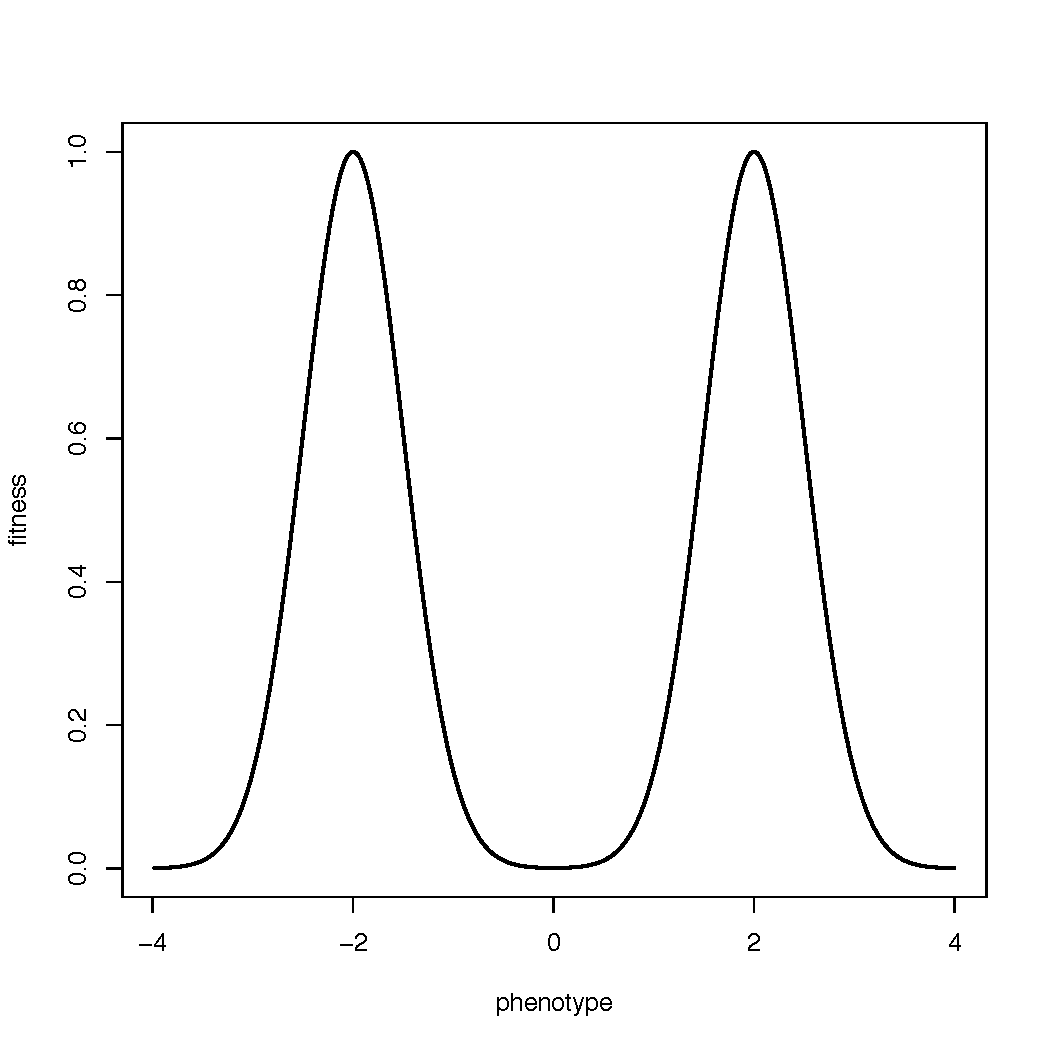
\includegraphics[width=0.70\textwidth]{fitness-landscape-selection.pdf}
    \label{fig:fitness-landscape-selection}
\end{figure}

The fitness landscape is defined by two tightly linked parameters:

\begin{description}
\item[quanti\_phenotype\_landscape\index{quanti\_phenotype\_landscape}]\hspace*{\fill}\\
\vspace{-9mm}
\item[quanti\_phenotype\_landscape\_fem\index{quanti\_phenotype\_landscape\_fem}]\hspace*{\fill}\\
\vspace{-9mm}
\item[quanti\_phenotype\_landscape\_mal\index{quanti\_phenotype\_landscape\_mal}]\textbf{[decimal/matrix] (temporal/default: 0)}\\
These parameters allow to specify an array of phenotypes for which the corresponding fitness is defined using the parameter \textsf{quanti\_fitness\_landscape}.  The phenotype values are either specified by a single value (similar to the default value) specifying a unique phenotype for all patches and quantitative traits together (all phenotypes will result in the same fitness), or by a one dimensional array (1D matrix) specifying the same fitness landscape for all patches and a given quantitative traits together, or by a 2D matrix specifying the fitness landscape separately for each patch for a given quantitative trait. Since the two parameters \textsf{quanti\_fitness\_phenotype} and \textsf{quanti\_fitness\_fitness} are tightly linked, \textit{i.e.} specify the phenotypes and their corresponding fitness values, the architecture of the two parameters have to be identical, \textit{i.e.} show up the same number of values for a patch. 


\item[quanti\_fitness\_landscape\index{quanti\_fitness\_landscape}]\hspace*{\fill}\\
\vspace{-9mm}
\item[quanti\_fitness\_landscape\_fem\index{quanti\_fitness\_landscape\_fem}]\hspace*{\fill}\\
\vspace{-9mm}
\item[quanti\_fitness\_landscape\_mal\index{quanti\_fitness\_landscape\_mal}]\textbf{[decimal/matrix] (temporal/default: 1)}\\
These parameters allow to specify the fitnesses corresponding to the phenotypes defined with the parameter \textsf{quanti\_phenotype\_landscape}, in the same order as the phenotypes are defined in the parameter \textsf{quanti\_fitness\_phenotype}. 
\end{description}

\paragraph{Example}\hspace*{\fill}
\begin{lstlisting}[frame=single]
quanti_phenotype_landscape {-4.0 -3.2 -2.4 -1.6 -0.8  0.0  
                             0.8  1.6  2.4  3.2  4.0}
quanti_fitness_landscape   {0.00 0.05 0.72 0.72 0.05 0.00 
                            0.05 0.72 0.72 0.05 0.00}    
\end{lstlisting}
In this example the selection pressure for all patches and quantitative traits are identical. The specified fitness landscape corresponds to the above shown figure, however, the resolution of the specification is reduced in the shown example. The binomial landscape is the sum of two stabilizing selections with optima set to -2 and 2 and an intensity of 0.5. 


\subsection{Selection coefficient}\label{sub:SelectionCoefficient}
QuantiNemo supports the simulation of bi-allelic loci where the selection pressure is defined by a selection coefficient. In this simplified, but widespread model, the genotype is directly mapped to a fitness:\\

\begin{tabular}{ccc}
 \hline            
Genotype & Fitness & Fitness extended \\
\hline
AA & 1             & F      \\
Aa & 1 - hs & F - hs \\
aa & 1 - s     & F - s  \\
\hline
\end{tabular}

Where $s$ is the selection coefficient (parameter \textsf{quanti\_coef\_sel}), $h$ the dominance factor (parameter \textsf{quanti\_dominance\_mean}) with the model (parameter \textsf{quanti\_dominance\_model}) set to 1 ($h$-model, has to be set explicitly!), and $F$ is the fitness factor for the wild type genotype $AA$ set by parameter \textsf{quanti\_coef\_sel\_AA}. This latter parameter is normally not used therefore it is listed in the column ``Fitness extended``.
\begin{description}
\item[quanti\_coef\_sel\index{quanti\_coef\_sel}]\hspace*{\fill}\\
\vspace{-9mm}
\item[quanti\_coef\_sel\_fem\index{quanti\_coef\_sel\_fem}]\hspace*{\fill}\\
\vspace{-9mm}
\item[quanti\_coef\_sel\_mal\index{quanti\_coef\_sel\_mal}]\textbf{[decimal/matrix] (temporal/default: 0)}\\
These parameters allow to set the selection coefficient $s$ for each patch and quantitative trait/locus. The default value of 0 will result in equivalent fitness for both alleles, and thus no selection acts.

\item[quanti\_coef\_sel\_AA\index{quanti\_coef\_sel\_AA}]\hspace*{\fill}\\
\vspace{-9mm}
\item[quanti\_coef\_sel\_AA\_fem\index{quanti\_coef\_sel\_AA\_fem}]\hspace*{\fill}\\
\vspace{-9mm}
\item[quanti\_coef\_sel\_AA\_mal\index{quanti\_coef\_sel\_AA\_mal}]\textbf{[decimal/matrix] (temporal/default: 1)}\\
These parameters allow to set the fitness for the wild type genotype $AA$ for each patch and quantitative trait/locus. By default it is 1.
\end{description}

\section{Selection level and position}
\subsection{Selection level}
With the following parameters it is possible to define the level of selection.

\begin{description}
\item[selection\_level\index{selection\_level}] \textbf{[0-3] (default: 0)}\\
This parameter specifies how selection acts at the reproduction stage. 
\begin{description}
\item [0~:~soft selection.] $nbOff_{p} = N_{p}$\\
The fitness of an individual is relative to the mean fitness of the population of its patch (soft selection at the patch level). This means that the population size does not depend on the mean fitness of the population and that selection does act locally at the patch level, \textit{i.e.} patches do not interact \citep{Wallace_1975}. No populations may therefore go extinct due to their maladaptation.

\item [1~:~metapopulation selection.] $nbOff_{p} = (W_{p}/W_{m})N_{m}$\\
The fitness of an individual is relative to the mean fitness of the entire metapopulation (soft selection at the metapopulation level). This means that the size of the entire metapopulation does not depend on the mean fitness. However, the population size of each patch depends on the mean fitness of its population \citep{Ravigne_2004}. This implies that a well adapted population grows while the population size of a less adapted population declines. Individual populations may go extinct due to their maladaptation, however not the entire metapopulation. 

\item [2~:~hard selection .] $nbOff_{p} = \bar{W}_{p}*N_{p}$\\
The fitness of an individual is absolute. If selection acts at reproduction the number of offspring to produce is scaled by the mean fitness of the population (the maximum number of offspring to produce (with a mean fitness of 1) is defined by the parameter \textsf{mating\_nb\_offspring}). If selection acts during regulation then the fitness of an individual is identical to its survival probability. Only with hard selection, the entire metapopulation may go extinct if the populations are maladapted. 


\end{description}

The shown equation are correct for selection during reproduction and deviate slightly if selection acts at another stage. $nbOff_{p}$ is the number of offspring to be produced in patch $p$, $N_{p}$ and $N_{m}$ are the total number of offspring defined by the parameter \textsf{mating\_nb\_offspring\_model} of patch $p$ and metapopulation $m$, respectively, $W_{p}$ and $W_{m}$ are the sum of fitnesses of patch $p$ and metapopulation $m$, respectively, and $\bar{W}_{p}$ is the mean fitness of patch $p$. 


Here is an example of the different selection levels in case of selection at the reproductive success. Both populations have a carrying capacity ($K$) of 1000 individuals, the parameter \textsf{mating\_nb\_model} is set to 0, and the mean fitnesses of the populations ($\bar{W}$) are 0.6 and 0.2, respectively:\\
\begin{tabular}{llll}
 \hline             & population 1    & population 2   & \\ 
                    & $K = 1000$      & $K = 1000$     & \\
 selection level&   $\bar{W} = 0.6$ & $\bar{W} = 0.2$& total\\
 \hline
 soft               & 1000            & 1000           & 2000\\
 metapopulation     & 1500            & 500            & 2000\\
 hard               & 600             & 200            & 800\\
 \hline
\end{tabular}

\item[patch\_mean\_fitness\index{patch\_mean\_fitness}] \textbf{[0-2] (default: 0)}\\
This parameter specifies how the mean fitness of a patch is defined. By default, all individuals are considered.
\begin{description}
\item [0~:~all.] The fitness of all individuals (females and males) is considered (default).
\item [1~:~only females] Just the fitness of the females is considered.
\item [2~:~only males] Just the fitness of the males is considered.
\end{description}
\subsection{Selection position}
By default, the selection appends during breeding. This is a reasonable choice for performance issue (all individual created go until the next reproduction stage, \textit{i.e.} no "useless" individuals are created). However, quantiNemo also offer the possibility for selection to act at other stages of the life cycle. Note, however, that selection may only act at a single stage at once. 
\item[selection\_position\index{selection\_position}] \textbf{[0-4] (default: 0)}\\
The parameter specifies when and how selection acts. By default, selection acts at reproduction where the fecundity of an individual depends on its fitness.
\begin{description}
\item [0~:~reproductive success.] Selection acts at the reproduction stage (see section \ref{sec:MatingSystem}), where the number of offspring of an individual depends on its fitness.
\item [1~:~reproductive success special.] Currently not working (do not use). 
\item [2~:~offspring survival.] Selection acts at the survival probability of the offspring, \textit{i.e.} before dispersal (see section \ref{sec:RegulationOffspring}).
\item [3~:~adult survival.] Selection acts at the survival probability of the adults, \textit{i.e.} after dispersal (see section \ref{sec:RegulationAdults}).
\item [4~:~no selection.] This option allows performing simulations without any selection.
\end{description}


\end{description}

\section{Fitness factor}
\label{sec:FitnessFactor}
The fitness factor allows translating a genotype directly into a fitness value. A fitness factor may be set either at the quantitative trait genotype level, at the locus level or globally for homozygote and/or heterozygote loci. The resulting fitness factor is determined in the above mentioned order, first quantitative trait genotype specific settings are considered, followed by locus specific settings and finally global parameters. The default fitness factor is 1 for all cases. This feature of quantiNemo allows among others to simulate recessive deleterious alleles, heterozygote or homozygote deficits, or incompatibilities of alleles for example to simulate hybridization or speciation. 

\subsection{Fitness factor at locus level}
The fitness factors at the locus level are defined in the dominance file (see section \ref{sub:DominanceEffects})
\subsection{Fitness factor at trait level}
The fitness factors at the trait level are defined in the epistatic file (see section \ref{sub:EpistaticEffects})
\subsection{Fitness factor at global level}
If the fitness factors are defined globally, the contribution to the fitness will be computed for each locus, and the final fitness will be obtained by multiplying the local fitnesses  To define the fitness factor globally the following parameters may be used:
    
\begin{description}
\item[quanti\_fitness\_factor\_heterozygote\index{quanti\_fitness\_factor\_heterozygote}] \textbf{[decimal/matrix] (default: 1)}\\
This parameter allows to specify the fitness factor for heterozygote loci, \textit{i.e.} if the two alleles at a given locus are different. Using a matrix it is possible to define different fitness factors for each locus. By default the fitness factor for heterozygote loci is 1, resulting in no effect on the fitness. 

\item[quanti\_fitness\_factor\_homozygote\index{quanti\_fitness\_factor\_homozygote}] \textbf{[decimal/matrix] (default: 1)}\\
This parameter allows to specify the fitness factor for homozygote loci, \textit{i.e.} if the two alleles at a given locus are identical. Using a matrix it is possible to define different fitness factors for each locus. By default the fitness factor for homozygote loci is 1, resulting in no effect on the fitness. 

\end{description}


%%%%%%%%%%%%%%%%%%%%%%%%%%%%%%%%%%%%%%%%%%%%%%%%%%%%%%%%%%%%%%%%%%%%%%%%%%%%%%%%%%%%%%%%%%%%%%%%%%%%%%%%%%%%%%%%%%%%%%%%%%%%%%%%%%%%%%
\newpage


\chapter{Coalescence}\label{chap:Coalescence}
\section{Introduction}
QuantiNemo has been developed to perform forward in time simulations at the individual level. This allows simulating realistically highly complex quantitative traits under selection. The drawback of this type of simulation is the huge demand of memory and long computation times. In contrast, population-based backward in time simulations based on the coalescence theory are much more efficient in terms of computation time and memory usage but do not allow to simulate realistic quantitative traits under selection. In order to take advantage of both types of simulations, we have added a layer of coalescence to quantiNemo2. Having both individual and population-based simulations allow for the user to switch easily the simulation mode depending on the type of simulation, keeping all the rest of the simulation/demography identical. 

This allows, for example, to explore a demographic history using efficient population-based simulations and then to make the simulations more realistic by switching to individual based simulations. Technically the population-based simulations simulate forward in time the evolution of the entire populations. During this simulation, the population sizes and immigration rates for all patches are stored in an internal database. In a second step, the database is used to simulate backward in time corresponding coalescence trees on which in a third step the mutations are sprinkled to generate the genetic polymorphism.
Most of the parameters of quantiNemo may be used in both simulation modes, but not all. Thus it is not possible to simulate any quantitative traits and thus no selection acts in population-based simulations. It is also important to note that population sizes in coalescence simulations are effective population sizes, whereas in individual-based simulation census population sizes. In addition at the current stage, the coalescence simulations are limited to hermaphrodite individuals and unlinked neutral markers. The genetic maps is not taken into account in the population-based mode. Finally, statistics are only available for adults, since only the last generation of individuals is created. 

In this chapter, the coalescence specific parameters are described.

\begin{description}
\item[coalescence\index{coalescence}] \textbf{[0-1] (default: 0)}\\ 
This parameter allows to switch between forward-in-time simulation of individuals and backward-in-time simulations of populations (coalescence):
\begin{description}
\item[0~:~individual based.] Forward-in-time simulation of individuals. That is the default mode where quantitative traits and selection may be simulated. 
\item[1~:~population based.] Backward-in-time simulations of populations using a coalescence approach. Only able to generate unlinked neutral markers.
\end{description}

\item[coalescence\_model\_threshold\index{coalescence\_model\_threshold}] \textbf{[decimal] (default: 0.1)}\\ 
The probability $p$ that a single coalescence event per generation and patch occurs depends on the number of traced lineages $n$ and the population size $N$ (in diploid numbers):
    \[
    p = \frac{n(n-1)}{4N}.
\]  
This approximation is valid for small numbers of traced lineages compared to the population size ($n<<N$). If $n$ in relation to $N$ gets bigger the probability that more than one coalescence event occurs increases and thus the method above is not any more accurate. Therefore quantiNemo allows setting a threshold (this parameter) for the probability of a single coalescence even $p$ above which the method used to simulate the coalescence events is changed. In this latter case the coalescence process is simulated realistically, \textit{i.e.} for each traced lineage a parental gene is drawn randomly. All lineages with an identical parental gene are then coalesced. In this case, at each generation, several coalescence events may happen but also events involving the fusion of three or more lineages are possible. 

This method is always valid, however much slower in terms of computation time than the previously mentioned one (Note however that this is still much faster than forward in time simulation). By default the value of this parameter, \textit{i.e.} the threshold, is set to 0.1 which is an acceptable threshold. Note that the probability that a single coalescence event occurs may exceed extensively 1. A value of 0 implies that the coalescent process is always realistically simulated. And ratios above 0 are used to specify the threshold below which a singe coalescence event is assumed and above which the coalescence process is simulated realistically. A parameter value of 1e6 is arbitrarily used to tell quantiNemo that only single coalescence events should be assumed.    

\item[divergence\_time\index{divergence\_time}] \textbf{[integer] (default: 0)}\\ 
A coalescence simulation lasts until the most recent common ancestor (MRCA) is reached. Depending on the simulated demography the MRCA may be found within the simulated time, but it can well be that the MRCA of all sampled lineages lays before the start of the demographic simulation. In this case, going backward in time the coalescence simulation is continued behind the demographic simulation assuming no migration between the remaining patches. At the divergence time (parameter \textbf{divergence\_time} all remaining lineages are then merged to a single patch of specified size (parameter \textbf{divergence\_pop\_size} below). By default the value of the parameter \textbf{divergence\_time} is 0. If the divergence time is set to less than the number of simulated generations (as the default) the divergence time will be readjusted to the number of generations, thus all remaining lineages are merged to a single patch when the onset of the demographic simulation is reached. 

\item[divergence\_pop\_size\index{divergence\_pop\_size}] \textbf{[integer] (default: 0)}\\ 
This parameter allows to define the final population size after the divergence time. Check the parameter \textbf{divergence\_time} for a description of it. If the argument is 0 (default value) the population size is adjusted to the current total number of individuals. If the specified population size is smaller than the number of traced lineages, then the population size is increased to the smallest possible population size still capable to carry the traced lineages. 
\end{description} 
 

\section{Output}
The coalescence simulations allow to output the coalescence trees and also the times to the MRCA.

\subsection{Trees}\label{coalTrees}
The coalescence trees may be dumped to file in the NEXUS format. The branches of the tree may be either scaled by the coalescence times, or by the number of mutations. Several programs allowing to visualize NEXUS files such as for example FigTree developed by Andrew Rambaut \url{www.tree.bio.ed.ac.uk/software/figtree}. The NEXUS file has the extension \textbf{.tree}.

\begin{description} 
\item[coalescence\_save\_tree\index{coalescence\_save\_tree}] \textbf{[0-2] (default: 0)} \\
This parameter specifies the output of the coalescence trees.
\begin{description}
\item [0 : None.] No output is generated.
\item [1 : scaled by coalescence time.] The trees are outputted in the NEXUS format and branches are scaled by the coalescence times.
\item [2 : scaled by number of mutations.] The topology of the trees is the same as before, but the branches are now scaled by the number of mutations.
\end{description} 

An example of a tree file for 3 loci and 3 sampled diploid individuals:
\begin{lstlisting}[frame=single]
#NEXUS

[Treefile generated by quantiNemo
    quantiNemo v1.5.0[May 20 2010; 09:14:19]
    File created the 20-05-2010 09:14:27
    Branches are scaled by the coalescence time
]

Begin trees;

Translate
    1 1a,
    2 1b,
    3 2a,
    4 2b,
    5 3a,
    6 3b;

tree LOCUS_1 = ((5: 114, 4: 114): 2, ((1: 59, 6: 59): 2, (3: 13, 2: 13): 48): 55);
tree LOCUS_2 = (1: 72, ((6: 33, 5: 33): 22, ((2: 3, 4: 3): 2, 3: 5): 50): 17);
tree LOCUS_3 = (((1: 9, 2: 9): 13, 6: 22): 209, ((4: 0, 5: 0): 180, 3: 180): 51);

End;
\end{lstlisting}

\item[coalescence\_tree\_dir\index{coalescence\_tree\_dir}] \textbf{[string] (default: "")}\\
This parameter allows to specify the subdirectory where the tree files are stored. This directory has to be specified relative to the simulation folder (parameter \textsf{folder}), and may also contain subdirectories. If not specified (default) the output is stored in the simulation folder (parameter \textsf{folder}).

\item[coalescence\_tree\_filename\index{coalescence\_tree\_filename}] \textbf{[string] (default: "")}\\
This parameter is used to specify an individual base filename for the coalescence trees. If not specified the generic base filename will be used (see parameter \textsf{filename}).


\item[coalescence\_tree\_script\index{coalescence\_tree\_script}] \textbf{[string] (default: "")}\\
It is possible to launch a script just after the tree file is generated. The argument of the parameter is the file name of the script. The name of the tree file is passed as unique parameter to the script. 
\end{description}


\subsection{MRCA}\label{coalMRCA}
The times to the MRCA may be dumped to file as a simple list. The file has the extension \textbf{.mrca}.

\begin{description} 
\item[coalescence\_save\_mrca\index{coalescence\_save\_mrca}] \textbf{[0-1] (default: 0)} \\
This parameter specifies whether the times to the MRCA are outputted.
\begin{description}
\item [0 : None.] No output is generated.
\item [1 : Output.] The times to the MRCA are outputted.
mutations.
\end{description} 

An example of such a file for 3 loci is:
\begin{lstlisting}[frame=single]
112
339
813
\end{lstlisting}

\item[coalescence\_mrca\_dir\index{coalescence\_mrca\_dir}] \textbf{[string] (default: "")}\\
This parameter allows to specify the subdirectory where the MRCA files are stored. This directory has to be specified relative to the simulation folder (parameter \textsf{folder}), and may also contain subdirectories. If not specified (default) the output is stored in the simulation folder (parameter \textsf{folder}).

\item[coalescence\_mrca\_filename\index{coalescence\_mrca\_filename}] \textbf{[string] (default: "")}\\
This parameter is used to specify an individual base filename for the coalescence MRCA. If not specified the generic base filename will be used (see parameter \textsf{filename}).

\item[coalescence\_mrca\_script\index{coalescence\_mrca\_script}] \textbf{[string] (default: "")}\\
It is possible to launch a script just after the MRCA file is generated. The argument of the parameter is the file name of the script. The name of the MRCA file is passed as unique parameter to the script. 
\end{description}

\subsection{Lineages}\label{coalLineages}
For the coalescence simulation, it is possible to dump the current populated patches, including their population sizes and number of traces lineages to a file for any given generation. The file is generated for each locus separately and has the ending \textbf{\_lX.lin}, where $X$ is the locus index. The format is as follows: Each line contains a single generation, \textit{i.e.} time slice. The line starts with the generation index relative to the start of the simulation. Thus since the coalescence simulations are proceeded backward in time the generations decrease from top to down of the file. Positive numbers are time slices where a demographic simulation is available and negative numbers for time slices before (forward in time) the demographic simulation. The generation number is followed by the total number of currently traced lineages. Then each populated patch is listed using three numbers, the patch index, the current population size, and the current number of traced lineages. Since over time some patches may be colonized or freed the number of columns per line may change between generations.

\begin{description} 
\item[coalescence\_save\_lineages\index{coalescence\_save\_lineages}] \textbf{[0-1] (default: 0)} \\
This parameter specifies whether the patch stages are outputted.
\begin{description}
\item [0 : None.] No output is generated.
\item [1 : Output.] The patch stages are outputted.
\end{description} 

\item[coalescence\_lineages\_logtime\index{coalescence\_lineages\_logtime}] \textbf{[integer] (temporal/default: 1)}\\
This parameter allows to specify at which generations DURING the period of the demographic simulation the patch stages are dumped to file. 

\item[coalescence\_lineages\_logtime2\index{coalescence\_lineages\_logtime2}] \textbf{[integer] (temporal/default: 1)}\\
This parameter allows to specify at which generations BEFORE (forward in time) the demographic simulation the patch stages are dumped to file. 

\item[coalescence\_save\_lineages\_dir\index{coalescence\_save\_lineages\_dir}] \textbf{[string] (default: "")}\\
This parameter allows to specify the subdirectory where the lineages files are stored. This directory has to be specified relative to the simulation folder (parameter \textsf{folder}), and may also contain subdirectories. If not specified (default) the output is stored in the simulation folder (parameter \textsf{folder}).

\item[coalescence\_save\_lineages\_filename\index{coalescence\_save\_lineages\_filename}] \textbf{[string] (default: "")}\\
This parameter is used to specify an individual base filename for the lineages files. If not specified the generic base filename will be used (see parameter \textsf{filename}).

\item[coalescence\_lineages\_script\index{coalescence\_lineages\_script}] \textbf{[string] (default: "")}\\
It is possible to launch a script just after the patch stage file is generated. The argument of the parameter is the file name of the script. The name of the patch stage file is passed as unique parameter to the script. 
\end{description}

\subsection{Population sizes}\label{coalPopSizes}
For the coalescence simulation, it is possible to dump the current populated sizes to file. The format of the file is the generation time followed by the population sizes for the patches of choice.

\begin{description} 
    \item[coalescence\_save\_pop\_sizes\index{coalescence\_save\_pop\_size}] \textbf{[0-1] (default: 0)} \\
    This parameter specifies whether the population sizes are outputted.
    \begin{description}
        \item [0 : None.] No output is generated.
        \item [1 : Output.] The population sizes are outputted.
    \end{description} 
    
    \item[coalescence\_pop\_sizes\_logtime\index{coalescence\_pop\_sizes\_logtime}] \textbf{[integer] (temporal/default: 1)}\\
    This parameter allows to specify at which generations the population sizes are dumped to file. 
    
\item[coalescence\_save\_pop\_sizes\_dir\index{coalescence\_save\_pop\_sizes\_dir}] \textbf{[string] (default: "")}\\
This parameter allows to specify the subdirectory where the population sizes files are stored. This directory has to be specified relative to the simulation folder (parameter \textsf{folder}), and may also contain subdirectories. If not specified (default) the output is stored in the simulation folder (parameter \textsf{folder}).

\item[coalescence\_save\_pop\_sizes\_filename\index{coalescence\_save\_pop\_sizes\_filename}] \textbf{[string] (default: "")}\\
This parameter is used to specify an individual base filename for the population sizes files. If not specified the generic base filename will be used (see parameter \textsf{filename}).

    \item[coalescence\_pop\_sizes\_of\_patch\index{coalescence\_pop\_sizes\_of\_patch}] \textbf{[integer/matrix] (default: "")}\\
    This parameter allows defining the patches for which the population sizes should be outputted using a matrix with the patch IDs. By default the population sizes of all patches is outputted.
    \item[coalescence\_pop\_sizes\_script\index{coalescence\_pop\_sizes\_script}] \textbf{[string] (default: "")}\\
    It is possible to launch a script just after the population sizes file is generated. The argument of the parameter is the file name of the script. The name of the population size file is passed as unique parameter to the script. 

\end{description}

\section{Summary statistics}\label{sec:SummaryStatistics_coalescence}
The summary statistics listed in the table below are available for coalescence simulations. The column \textsf{Stat name} contains the name of the summary statistic used to specify which summary statistics are computed (parameter \textsf{stat}, for details see section \ref{sec:SummaryStatistics}). These names appear also in the output file. The column \textsf{Description} contains a short description of the summary statistic. 

The summary statistic name (column \textsf{Stat name}) may be used to specify the summary statistic to be computed (e.g. \textsf{mrca.mean}). Similar summary statistics (within a thematic group) may be obtained at once using the name within square brackets after the group title (e.g. \textsf{mrca}). Using this group statistic name all summary statistics of the thematic group marked with a star (*) will be computed. 
\\
\\
\begin{description}
\item[sample\_all\_or\_nothing\index{sample\_all\_or\_nothing}] \textbf{[0,1] (default: 0)}\\
This parameter allows to specify when statistics should be computed (only available for the coalescence simulations ):
\begin{description}
\item[0~:~when possible.] In this case statistics and outputs are generated whenever it is possible, \textit{i.e.} whenever a patch is enough populated that a given statistic may be computed.
\item[1~:~all or nothing.] In this case statistics and output are generated only if the entire sampling schema may be applied, \textit{i.e.} if the patches are enough populated that the specified sampling may be applied. If this is not the case a NaN or a zero depending on the statistic is outputted for all statistics. Note that in such a case the genetic part of the coalescence simulations are omitted, thus the simulation may be much quicker although useless. A specified sampling may not be applied if (and only if) not all specified patches (parameter \textsf{sampled\_patches} defined as a matrix) may be sampled or the population size is inferior to the sampling size (parameter \textsf{patch\_sample\_size} defined in entire numbers (absolute)).
\end{description}
\end{description}
\topcaption{\label{coalstats}Summary statistics available for coalescence simulations}
\tablehead{\hline \multicolumn{2}{l}{Stat name} &Description \\ \hline}
\tabletail{\hline \multicolumn{3}{l}{\emph{Table \ref{coalstats} continued on next page}} \\}
\tablelasttail{\hline \multicolumn{3}{l}{\emph{Table \ref{coalstats}: Summary statistics available for coalescence simulations continued}}}
\begin{supertabular}{G}
\multicolumn{3}{l}{\emph{MRCA} [mrca]}\\
 &mrca.mean            &mean time to the MRCA*\\
 &mrca.var            &variance of the time to the MRCA* \\
\end{supertabular}





\chapter{Ouputs and Statistics}
\label{chap:OutputsAndStatistics}
QuantiNemo allows to output summary statistics as well as raw data about the population, including the complete genome, in order to offer the highest flexibility. QuantiNemo can also output log files to resume a simulation or restart it from the beginning with the same random parameter. More precisely, quantiNemo can output:
\begin{description}
\item[summary statistics]\hspace*{\fill}\\
QuantiNemo provides summary statistics for the different simulation components, including for example genetic variance estimates, quantitative trait analysis (e.g. $Q_{ST}$), and F-statistics. The summary statistics can be computed for any generation during the simulation. If several replicates are performed, the averaged across replicates as well as the value for each replicate can be outputted. 

\item[raw data]\hspace*{\fill}\\
QuantiNemo can also produce files with the raw genetic and phenotypic data. The genotypes at all loci can be dumped to file in the FSTAT  \citep{Goudet_1995} or Arlequin format \citep{Excoffier_2010}. Phenotypes, as well as the additive, dominance, and epistatic effect values can be written to a file and then analyzed with any population or quantitative genetic software, e.g. to get patterns of differentiation, study linkage disequilibrium, or scan for QTL. Genotypes and phenotypes can be saved for any generation during the simulation.

\item[log files]\hspace*{\fill}\\
QuantiNemo also generates log files allowing to reconstruct performed simulations. There are two types of log files. The first log file records the simulations performed with quantiNemo and stores some general information. This log file is stored in the folder of the executable and allows to reconstruct the chronology of performed simulations and their main features. The other log file contains the used parameters, is generated for each simulation separately and is stored in the simulation folder. This file is in principle a copy of the used settings file and contains the starting time and the duration time of the simulation. It contains also the seed (see parameter \textsf{seed}) used to initialize the simulation. This file can be used as settings file to exactly repeat the performed simulation. Note, that due to the seed in the file the random generator will be initialized in the same way leading to the exact same values in the output.
\end{description}


\section{Files name}
All files of a simulation are stored in a unique folder (see parameter \textsf{folder}). This simulation folder may contain a substructure. The names of the output files are based on the base name given by the parameter \textsf{filename}. Depending on the type of output different extensions are added to the base name. To avoid that recurring outputs overwrite previous outputs a counter is added to the file name between base name and extension. There are two types of counters: the generation counter and the replication counter. A counter is only added if there is a risk of overwriting. For example, the replication counter is only added if several replications are performed. The generation counter starts with "\_g" and the replication counter with "\_r". These characters are followed by the number of the generation and replication, respectively. Note, that generations and replications start at 1. The number has as many digits as are needed to represent the highest number in the simulation: 

\begin{lstlisting}[frame=single]
simulation_g0001_r01.dat
simulation_g0002_r01.dat
...
simulation_g5000_r10.dat
\end{lstlisting}
\section{Sampling}\label{sec:Sampling}
By default, the outputs generated by quantiNemo (summary statistics, genotypes, phenotypes, and genotypic values) are computed/outputted considering all individuals and populations. This section describes parameters allowing to constrain the considered populations and/or individuals. The parameter \textbf{sampled\_patches} allows to make a pre-selection on the patches, whereas the parameter \textbf{patch\_sample\_size} allows defining for each patch and/or sex the sampled number of individuals. It is therefore possible to specify the samples just using the parameter \textbf{patch\_sample\_size}.
 
\begin{description}
\item[sampled\_patches\index{sampled\_patches}] \textbf{[integer/matrix] (default: 0)}\\ 
The parameter \textbf{sampled\_patches} allows defining a sampling schema for patches, where ALL individuals are sampled. There are different methods to define the sampled patches:
\begin{description}
\item[single number.] If the argument is a single number the patches to sample are drawn randomly. In this case, the passed number specifies the total number of patches to sample. Patches are drawn randomly for each replicate but remain the same during a simulation. A special case is 0 as argument (default value). In this case, all patches are sampled. 
\item[matrix.] Using a one dimensional matrix as argument allows to define explicitly the patches to sample. Please note that for this parameter a matrix has to be defined fully, \textit{i.e.} all patches to sample have to be listed in the matrix and a single number is not expanded to a matrix. Note, that in contrast to the normal matrix behaviour the two arguments \textit{20} and \textit{\{20\}} are not identical. While the former one is considered as a single number defining the total number of sampled patches, the second one is a matrix and defines the patch to be sampled, \textit{i.e.} patch 20.  
\end{description}

\item[patch\_sample\_size\index{patch\_sample\_size}]\hspace*{\fill}\\
\vspace{-9mm}
\item[patch\_sample\_size\_fem\index{patch\_sample\_size\_fem}]\hspace*{\fill}\\
\vspace{-9mm}
\item[patch\_sample\_size\_mal\index{patch\_sample\_size\_mal}]\textbf{[decimal/matrix] (temporal/default: NaN)}\\
These parameters allows to define for each patch and/or sex the sample size or sample proportion. Since the sampling schema may change over time the summary statistics are computed and outputted for all populations sampled at any time during the simulation even if at a given time the sample size is zero. These parameters here overwrite any settings specified by the parameter \textbf{sampled\_patches}.If the sampling is sex specific both sex specific parameters have to be set. The sampling for a single patch may be defined in the following ways:
\begin{description}
\item[proportion.] A decimal number (number between 0 and 1, exclusive 1) may be used to define the sample size relatively to the population size.
\item[absolute.] The sample size may be defined in an absolute number (1 or larger). If the absolute sample size exceeds the population size the entire population is sampled. 
\item[NaN.] This is the default argument and allows to sample all individuals of a population.
\end{description}

The sampling schema for all patches may be defined as follows:
\begin{description}
\item[single number.] All patches have the same sampling schema, \textit{i.e.} sampling proportion or sampling number.
\item[1D matrix.] The sample sizes/proportions of each patch may be set using a 1D matrix. The setting of this matrix behaves as the matrix for the parameter \textbf{patch\_capacity} or \textbf{patch\_ini\_size}, \textit{i.e.} the matrix size is adjusted if needed. Within a matrix, the individual patch sample sizes may vary between relative, absolute, or \textit{NaN} definitions. 
\item[2D matrix.] A 2D matrix allows specifying directly the sample sizes/proportions for a given number of patches. The number of columns has to be 2, where the first column contains the patch ID and the second column the corresponding sampling number/proportion. Within a matrix, the individual patch sample sizes may vary between relative, absolute, or \textit{NaN} definitions. All not specified patches will not be sampled, \textit{i.e.} have a sample size of 0.
\end{description}
\end{description}
\section{Summary statistics}\label{sec:SummaryStatistics}
It is possible to record summary statistics specified by the parameter \textsf{stat}. At the end of a simulation, the summary statistics are written to a text file. By default, the summary statistics are printed individually per replicate and/or summed up across replicates (mean and variance across replicates). In this latter case an additional statistic named \textit{alive.rpl} will be added which contains the number of alive replicates, \textit{i.e.} the number of simulations where the populations did not get extinct. It is also possible to set the frequency (parameter \textsf{stat\_log\_time}) of the recording, which reduces the simulation time and the size of the output file. 


Some of the summary statistics are available for adults and offspring (indicated by \textsf{(adlt/off)}). To obtain a certain summary statistic for adults the prefix \textsf{adlt.} has to be added to the summary statistic name (e.g. \textsf{adlt.allnb}), respectively the prefix \textsf{off.} to obtain the summary statistic for offspring (e.g. \textsf{off.allnb}). 

Relevant statistics can be computed either for the entire Metapopulation, or of every patch separately. In the latter case, the statistics are characterized by a suffix "\_p" to the \textsf{Stat name} and by the words \textit{(computed for each patch)} in the description of the statistic. Other summary statistics are computed for pairwise combinations of patches. These statistics are characterized by a suffix "\_pair" to the \textsf{Stat name} and by the words \textit{(all pairwise combinations computed)} in the description of the statistic. The names of such summary statistics in the output have the suffix "\_p\textit{X}" and "\_p\textit{X}-\textit{Y}", respectively. Where \textit{X} and \textit{Y} are the index of the patches (starting with 1). 

The summary statistics are computed by default for every trait. If several traits are simulated the postfix "\_t\textit{T}" is added to the summary statistic name in the output file, where \textit{T} is the index of the traits. It is possible to compute statistics just for specified traits. This can be specified by the index of the type inserted just after the \textit{(n)}. For example the stat option \textit(n.adlt.fst) computes the Fst for all types of neutral markers while the stat option \textit(n2.adlt.fst) computes the Fst just for the second neutral marker type. 




\begin{description}
\item[stat\index{stat}] \textbf{[string/matrix]}\\
This parameter allows specifying the summary statistics to be computed.  A exhaustive list of  existing statistics is given in the next subsection: \ref{sub:Demography}, \ref{sub:NeutralMarkers}, \ref{sub:QuantitativeTraits} (except for statistic specific to coalescence which are treated in the chapter about coalescence, section \ref{sec:SummaryStatistics_coalescence}). The arguments are keywords standing for one or multiple summary statistics. Keywords have to be written as a matrix within brackets separated by space. 

The summary statistic name (column \textsf{Stat name}) may be used to specify the summary statistic to be computed (e.g. \textsf{adlt.fst}). Similar summary statistics (within a thematic group) may be obtained at once using the name within square brackets after the group title (e.g. \textsf{adlt.fstat}). Using this group statistic name all summary statistics of the thematic group marked with a star (*) will be computed. 
\begin{lstlisting}[frame=single]
stat {n.fstat 
      quanti 
      adlt.demo}
\end{lstlisting}

\item[stat\_save\index{stat\_save}] \textbf{[0-6] (default: 0)}\\
This parameter specifies if the summary statistics should be computed and how they should be dumped to file. The summary statistics may be dumped to file for each specified generation and replicate separately (file "generic\_name\_stats.txt"), or summary statistics may be summed up across replicates by their mean (file "generic\_name\_stats.txt") and their variance (file "generic\_name\_var.txt").

The column \textsf{Stat name} contains the name of the summary statistic used to specify which summary statistics are computed. These names appear also in the output file. The column \textsf{Description} contains a short description of the summary statistic. 



\begin{description}

\item[0 : All.] Output includes all types of summary statistic (files "generic\_name\_stats.txt", "generic\_name\_mean.txt", and "generic\_name\_var.txt").
\item[1 : Detailed.] Output includes only the file containing the summary statistics for each replicate separately (file "generic\_name\_stats.txt"). Since in this case (in contrast to all other options) it is not necessary to save the statistics over all replicates, the statistics are written to file when they are computed. This means that the internal database to store the statistics is not used, consequently, the memory used by quantiNemo does not increase with each generation and replicate.
\item[2 : Summed up.] Output includes the files containing the summary statistics summed up by their mean and variance across replicates (files "generic\_name\_mean.txt", and "generic\_name\_var.txt"). 
\item[3 : Mean.] Output includes only the file containing the summary statistics summed up by their mean across replicates (file "generic\_name\_mean.txt").
\item[4 : Variance.] Output includes only the file containing the summary statistics summed up by their variance across replicates (file "generic\_name\_var.txt").
\item[5 : Median.] Output includes only the file containing the summary statistics summed up by their median across replicates (file "generic\_name\_median.txt").
\item[6 : None.] No summary statistics are written. The life cycle event "Statistics" is skipped.
\end{description}
Whenever the summary statistics are output (parameter \textsf{stat\_save} not set to 6) a file named "generic\_name\_legend.txt" containing a small description of the summary statistics is also generated.
 
\item[stat\_log\_time\index{stat\_log\_time}] \textbf{[integer] (temporal/default: 1)}\\
This is the time interval at which summary statistics are recorded. The interval must range between 1 and the number of generations. Since the parameter may change over time (temporal parameter) the summary statistics may be computed for any generation:
\begin{lstlisting}[frame=single]
stat_log_time (1 1, 10 10, 100 100) 
\end{lstlisting}
In this example for the first 9 generations the summary statistics are computed every generation, from the tenth until generation 99 they are computed at every tenth generation, and from the generation 100 every hundred generation. 

\item[stat\_dir\index{stat\_dir}] \textbf{[string] (default: "")}\\
This parameter is used to specify a subdirectory within the simulation folder (parameter \textsf{folder}) where the summary statistic files will be stored. If the parameter is not set, the files will be stored in the simulation folder.

\item[stat\_filename\index{stat\_filename}] \textbf{[string] (default: "")}\\
This parameter is used to specify an individual base filename for the statistics. If not specified the generic base filename will be used (see parameter \textsf{filename}).



\item[param\index{param}] \textbf{[string/matrix]}\\
This parameter allows specifying the parameter arguments to output together with the statistics. Note, the output is listed only in the detailed statistic file.

\item[stat\_NaN\index{stat\_NaN}] \textbf{[string] (default: "NaN")}\\
This parameter allows specifying a placeholder used for the output of the summary statistics for statistics which are not computable. By default the placeholder is \textit{NaN}. This default value is correctly read by the statistical package R when such a file is imported.

\end{description}
\subsection{Demography}
\label{sub:Demography}
\topcaption{\label{popstats}Summary statistics available for the demographic structure}
\tablehead{\hline \multicolumn{2}{l}{Stat name} &Description \\ \hline}
\tabletail{\hline \multicolumn{3}{l}{\emph{Table \ref{popstats} continued on next page}} \\}
\tablelasttail{\hline \multicolumn{3}{l}{\emph{Table \ref{popstats}: Summary statistics available for the demographic structure continued}}}
\begin{supertabular}{G}
\multicolumn{3}{l}{\emph{Demography} [(adlt/off).demo]} \\
 &(adlt/off).nbInd                    &total number of individuals in the metapopulation*\\
 &(adlt/off).nbFem                    &total number of females in the metapopulation*\\
 &(adlt/off).nbMal                    &total number of males in the metapopulation*\\
 &(adlt/off).meanInd                &mean number of individuals per inhabited patch*\\
 &(adlt/off).meanFem                &mean number of females per inhabited patch*\\
 &(adlt/off).meanMal                &mean number of males per inhabited patch*\\
 &(adlt/off).sexRatio              &sex ratio ($\frac{males}{females})$*\\
 &(adlt/off).nbPops           &number of inhabited patches*\\ 
 &(adlt/off).nbInd\_p                &number of individuals in patch $i$\\
 &(adlt/off).nbFem\_p                &number of females in patch $i$\\
 &(adlt/off).nbMal\_p                &number of males in patch $i$\\

\hline
\multicolumn{3}{l}{\emph{Demography of all individuals: In contrast to all other stats and outputs the following stats}}   \\
\multicolumn{3}{l}{\emph{consider all individuals and patches and not just the sampled ones.} [(adlt/off).demoTot]} \\
 &(adlt/off).nbIndTot             &total number of individuals in the metapopulation*\\
 &(adlt/off).nbFemTot              &total number of females in the metapopulation*\\
 &(adlt/off).nbMalTot                &total number of males in the metapopulation*\\
 &(adlt/off).meanIndTot            &mean number of individuals per inhabited patch*\\
 &(adlt/off).meanFemTot          &mean number of females per inhabited patch*\\
 &(adlt/off).meanMalTot         &mean number of males per inhabited patch*\\
 &(adlt/off).sexRatioTot    &sex ratio of individuals ($\frac{males}{females})$*\\
 &(adlt/off).nbPopsTot      &number of inhabited patches*\\ 
 &(adlt/off).nbIndTot\_p        &number of individuals in patch $i$\\
 &(adlt/off).nbFemTot\_p        &number of females in patch $i$\\
 &(adlt/off).nbMalTot\_p        &number of males in patch $i$\\

\hline
\multicolumn{3}{l}{\emph{Patch extinction} [ext.rate]} \\
 &ext.rate                                    &proportion of extinct patches in the metapopulation*\\
 
\hline
\multicolumn{3}{l}{\emph{Fecundity} [fecundity, available only for adults]} \\
 &fem.meanFec                    &mean realized female fecundity*\\
 &fem.varFec                        &mean variance of realized female fecundity*\\
 &mal.meanFec                    &mean realized male fecundity*\\
 &mal.varFec                        &mean variance of realized male fecundity*\\

\hline
\multicolumn{3}{l}{\emph{Kinship} [(adlt/off).kinship]} \\
 &(adlt/off).fsib                                &mean proportion of full-sib* \\
 &(adlt/off).phsib                                &mean proportion of paternal half-sib*\\
 &(adlt/off).mhsib                                &mean proportion of maternal half-sib*\\
 &(adlt/off).nsib                                &mean proportion of non-sib*\\
 &(adlt/off).self                                &mean proportion of selfed offspring*\\

\hline
\multicolumn{3}{l}{\emph{Migration} [migration, available only for adults]} \\
 &emigrants                                &mean number of emigrants per patch*\\
 &immigrants                            &mean number of immigrants per patch*\\
 &residents                                &mean number of residents per patch*\\
 &immigrate                                &mean effective immigration rate per patch* ($\frac{immigrants}{immigrants + residents}$)\\
 &colonisers                            &mean number of colonizers per extinct patch*\\
 &colon.rate                            &mean effective colonization rate of extinct patches*\\

\hline 
\multicolumn{3}{l}{\emph{Fitness} [fitness, available only for adults]} \\
 &VwW                                 &variance of the fitness of adults within patches*\\
 &VwB                                  &variance of the fitness of adults between patches*\\
 &meanW\_p                              &mean fitness of adults in patch $i$ (computed for each patch)\\
 &varW\_p                                  &variance of the fitness of adults in patch $i$ (computed for each patch)\\
 
\hline 
\multicolumn{3}{l}{\emph{Random number initialization} [seed]} \\
 &seed                                    &outputs all used seeds (not really a statistic)*\\
 
\end{supertabular} 


%%%%%%%%%%%%%%%%%%%%%%%%%%%%%%%%%%%%%%%%%%%%%%%%%%%%%%%%%%%%%%%%%%%%%%%%%%%%%%%%%%%%%%%%%%%%%%%%%%%%%%%%%%%%%%%%%%%%%%%%%%%%%%%%%%%%%%
\newpage

\subsection{neutral markers}\label{sub:NeutralMarkers}
\topcaption{\label{ntrlstats}Summary statistics available for neutral markers}
\tablehead{\hline \multicolumn{2}{l}{Stat name} &Description \\ \hline}
\tabletail{\hline \multicolumn{3}{l}{\emph{Table \ref{ntrlstats} continued on next page}} \\}
\tablelasttail{\hline \multicolumn{3}{l}{\emph{Table \ref{ntrlstats}: Summary statistics available for neutral markers continued}}}
\begin{supertabular}{G}
\multicolumn{3}{l}{\emph{Genotype coancestry} [n.(adlt/off).coa]}\\
 &n.(adlt/off).theta            &mean within patch coancestry*\\
 &n.(adlt/off).alpha            &mean between patch coancestry* \\
 &n.(adlt/off).thetaFF        &mean within patch, within females coancestry* \\
 &n.(adlt/off).thetaMM        &mean within patch, within males coancestry* \\
 &n.(adlt/off).thetaFM        &mean within patch, between sexes coancestry* \\
 &n.(adlt/off).coa.fsib        &mean coancestry within full-siblings*\\    
 &n.(adlt/off).coa.phsib    &mean coancestry within paternal half-siblings*\\    
 &n.(adlt/off).coa.mhsib    &mean coancestry within maternal half-siblings*\\    
 &n.(adlt/off).coa.nsib      &mean coancestry within non-siblings*\\    
 &n.(adlt/off).theta\_p      &mean coancestry within patch \textit{i} (computed for each patch)\\                                
 &n.(adlt/off).alpha\_pair&mean coancestry between patch \textit{i} and \textit{j} (all pairwise combinations computed)\\                                

\hline
\multicolumn{3}{l}{\emph{Genetic diversity} [n.(adlt/off).gendiv]}\\
 \multicolumn{3}{l}{\emph{number of alleles:}} \\
 &n.(adlt/off).nbAll           &mean across patches and loci*\\
 &n.(adlt/off).nbAll\_p     &mean across loci (computed for each patch)\\
 &n.(adlt/off).nbAll\_l     &mean across patches (computed for each locus)\\
 &n.(adlt/off).nbAll\_p\_l  &(computed for each patch and locus)\\
 &n.(adlt/off).nbAll.tot      &mean total across loci*\\
 &n.(adlt/off).nbAll.tot\_l    &total (computed for each locus)\\
 
 \multicolumn{3}{l}{\emph{number of fixed loci:}} \\
 &n.(adlt/off).nbFixLoc          &mean across patches and loci*\\
 &n.(adlt/off).nbFixLoc\_p     &mean across loci (computed for each patch)\\
 &n.(adlt/off).nbFixLoc\_l     &mean across patches (computed for each locus)\\
 &n.(adlt/off).nbFixLoc\_p\_l  &(computed for each patch and locus)\\
 &n.(adlt/off).nbFixLoc.tot       &mean total across loci*\\
 &n.(adlt/off).nbFixLoc.tot\_l &total (computed for each locus)\\
 
 \multicolumn{3}{l}{\emph{allele frequencies (caution: any potential allele is outputted!):}} \\
 &n.(adlt/off).a.freq      &local (computed for each patch, locus and allele)\\
 &n.(adlt/off).a.freq.global&global (computed for each locus and allele)\\
 
 \multicolumn{3}{l}{\emph{locus gentoype frequencies (caution: any potential allele combination is outputted!):}} \\
 &n.(adlt/off).l.freq      &local (computed for each patch, locus genotype)\\
 &n.(adlt/off).l.freq.global&global (computed for each locus genotype)\\
 
 \multicolumn{3}{l}{\emph{observed heterozygosity following \citet{Nei_1983}:}} \\
 &n.(adlt/off).ho              &*\\
 &n.(adlt/off).ho\_p    &(computed for each patch)\\
 &n.(adlt/off).ho\_l    &(computed for each locus)\\
 &n.(adlt/off).ho\_p\_l &(computed for each patch and locus)\\
 
 \multicolumn{3}{l}{\emph{expected heterozygosity following \citet{Nei_1983}:}} \\
 &n.(adlt/off).hs            &*\\
 &n.(adlt/off).hs\_p        &(computed for each patch)\\
 &n.(adlt/off).hs\_l        &(computed for each locus)\\
 &n.(adlt/off).hs\_p\_l    &(computed for each patch and locus)\\
 &n.(adlt/off).ht            &total*\\
 &n.(adlt/off).ht\_l    &total (computed for each locus)\\
 
 \multicolumn{3}{l}{\emph{expected heterozygosity ($H=1-\sum{p^{2}}$):}} \\
 &n.(adlt/off).hs.p2        &\\
 &n.(adlt/off).hs.p2\_p &(computed for each patch)\\
 &n.(adlt/off).hs.p2\_l    &(computed for each locus)\\
 &n.(adlt/off).hs.p2\_p\_l&(computed for each patch and locus)\\
 &n.(adlt/off).ht.p2        &total*\\
 &n.(adlt/off).ht.p2\_l &total (computed for each locus)\\
 
 \multicolumn{3}{l}{\emph{allelic richness following \citet{Mousadik_1996}:}} \\
 \multicolumn{3}{l}{\emph{(rarefaction is based on the smallest sample size)}} \\
 &n.(adlt/off).rs            &\\
 &n.(adlt/off).rs\_p        &(computed for each patch)\\
 &n.(adlt/off).rs\_l        &(computed for each locus)\\
 &n.(adlt/off).rs\_p\_l    &(computed for each patch and locus)\\
 &n.(adlt/off).rt            &total\\
 &n.(adlt/off).rt\_l    &total (computed for each locus)\\
 
 \multicolumn{3}{l}{\emph{allelic range (difference between min and max allele):}} \\
 &n.(adlt/off).r            &\\
 &n.(adlt/off).r\_p          &(computed for each patch)\\
 &n.(adlt/off).r\_l          &(computed for each locus)\\
 &n.(adlt/off).r\_p\_l    &(computed for each patch and locus)\\
 &n.(adlt/off).r.tot    &total\\
 &n.(adlt/off).r.tot\_l &total (computed for each locus)\\
 
 \multicolumn{3}{l}{\emph{garza-williamsons statistic following \citet{Garza_2001}:}} \\
 \multicolumn{3}{l}{\emph{(modification: $gw = \sum(nb.allele)/\sum(1+range)$)}} \\
 &n.(adlt/off).gw            &\\
 &n.(adlt/off).gw\_p        &(computed for each patch)\\
 &n.(adlt/off).gw\_l        &(computed for each locus)\\
 &n.(adlt/off).gw\_p\_l    &(computed for each patch and locus)\\
 &n.(adlt/off).gw.tot        &total\\
 &n.(adlt/off).gw.tot\_l&total (computed for each locus)\\ 
 
\hline
\multicolumn{3}{l}{\emph{F-statistics following \citet{Nei_1983}} [n.(adlt/off).fstat]}\\
 &n.(adlt/off).fst            &global $F_{ST}$*\\
 &n.(adlt/off).fst\_l        &global $F_{ST}$ (computed for each locus)\\
 &n.(adlt/off).fst\_pair&pairwise $F_{ST}$ between patch \textit{i} and \textit{j} (all pairwise combinations computed)\\
 &n.(adlt/off).fst\_pair\_l&pairwise $F_{ST}$ between patch \textit{i} and \textit{j} (all pairwise combinations computed for each locus separately)\\
 &n.(adlt/off).fis            &global $F_{IS}$*\\
 &n.(adlt/off).fis\_l        &global $F_{IS}$ (computed for each locus)\\
 &n.(adlt/off).fit            &global $F_{IT}$*\\
 &n.(adlt/off).fit\_l        &global $F_{IT}$ (computed for each locus)\\
 
\hline
\multicolumn{3}{l}{\emph{F-statistics following \citet{Weir_1984}} [n.(adlt/off).fstat.wc]}\\
 &n.(adlt/off).fst.wc            &global $F_{ST}$*\\
 &n.(adlt/off).fst.wc\_l    &global $F_{ST}$ (computed for each locus)\\
 &n.(adlt/off).fst.wc\_pair&pairwise $F_{ST}$ between patch \textit{i} and \textit{j} (all pairwise combinations computed)\\
 &n.(adlt/off).fst.wc\_pair\_l&pairwise $F_{ST}$ between patch \textit{i} and \textit{j} (all pairwise combinations computed for each locus separately)\\
 &n.(adlt/off).fis.wc          &global $F_{IS}$*\\
 &n.(adlt/off).fis.wc\_l    &global $F_{IS}$ (computed for each locus)\\
 &n.(adlt/off).fit.wc            &global $F_{IT}$*\\
 &n.(adlt/off).fit.wc\_l    &global $F_{IT}$ (computed for each locus)\\
 
\hline
\multicolumn{3}{l}{\emph{Linkage disequilibirum reviewed in \citet{Devlin_1995}}}\\
 &n.(adlt/off).Dprime              &global $Dprime$ (computed globally for each pair of loci)\\
 &n.(adlt/off).Dprime\_pair    &$Dprime_p$ (computed for each patch each pair of loci)\\
 &n.(adlt/off).Dstar              &global $Dstar$ (computed globally for each pair of loci)\\
 &n.(adlt/off).Dstar\_pair    &$Dstar_p$ (computed for each patch each pair of loci)\\
 &n.(adlt/off).R2                      &global $R2$ (computed globally for each pair of loci)\\
 &n.(adlt/off).R2\_pair            &$R2$ (computed for each patch and each pair of loci)\\
 &n.(adlt/off).Chi2                  &global $Chi2$ (computed globally for each pair of loci)\\
 &n.(adlt/off).Chi2\_pair        &$Chi2$ (computed for each patch and each pair of loci)\\
 
\hline
\end{supertabular}



\subsection{quantitative traits}\label{sub:QuantitativeTraits}

\topcaption{\label{quantistats}Summary statistics available for quantitative traits}
\tablehead{\hline \multicolumn{2}{l}{Stat name} &Description \\ \hline}
\tabletail{\hline \multicolumn{3}{l}{\emph{Table \ref{quantistats} continued on next page}} \\}
\tablelasttail{\hline \multicolumn{3}{l}{\emph{Table \ref{quantistats}: Summary statistics available for quantitative traits continued}}}
\begin{supertabular}{G}
\multicolumn{3}{l}{\emph{Quantitative trait statistics} [quanti, available only for adults]}\\
 &q.VgW                         &genetic variance within patches*\\
 &q.VgB                         &genetic variance between patches*\\
 &q.VpW                         &phenotypic variance within patches*\\
 &q.VpB                         &phenotypic variance between patches*\\
 &q.VaW                     &additive genetic variance within patches\\
 &q.qst                          &$Q_{ST}$\\
 &q.qst.f                        &$Q_{ST}$ corrected for inbreeding following \citet{Bonnin_1996}. Inbreeding coefficient \textit{F} computed following \citet{Nei_1983} \\
 &q.qst\_pair              &$Q_{ST}$ between patch \textit{i} and \textit{j} (all pairwise combinations computed)\\
 &q.qst.f\_pair         &$Q_{ST}$ between patch \textit{i} and \textit{j} (all pairwise combinations computed) corrected for inbreeding \\
 &q.varA\_p                  &additive genetic variance of patch $i$ following \citet[p85-87]{Lynch_1998} (computed for each patch)\\
 &q.meanG\_p              &genetic mean of patch $i$ (computed for each patch)\\
 &q.varG\_p                      &genetic variance of patch $i$ (computed for each patch)\\
 &q.meanP\_p                  &phenotypic mean of patch $i$ (computed for each patch)\\
 &q.varP\_p                      &phenotypic variance of patch $i$ (computed for each patch)\\

\hline
\multicolumn{3}{l}{\emph{Genotype coancestry} [q.(adlt/off).coa]}\\
 &q.(adlt/off).theta            &mean within patch coancestry*\\
 &q.(adlt/off).alpha            &mean between patch coancestry* \\
 &q.(adlt/off).thetaFF        &mean within patch, within females coancestry* \\
 &q.(adlt/off).thetaMM        &mean within patch, within males coancestry* \\
 &q.(adlt/off).thetaFM        &mean within patch, between sexes coancestry* \\
 &q.(adlt/off).coa.fsib        &mean coancestry within full-siblings*\\    
 &q.(adlt/off).coa.phsib    &mean coancestry within paternal half-siblings*\\    
 &q.(adlt/off).coa.mhsib    &mean coancestry within maternal half-siblings*\\    
 &q.(adlt/off).coa.nsib      &mean coancestry within non-siblings*\\    
 &q.(adlt/off).theta\_p      &mean coancestry within patch \textit{i} (computed for each patch)\\                                
 &q.(adlt/off).alpha\_pair &mean coancestry between patch \textit{i} and \textit{j} (all pairwise combinations computed)\\                                

\hline
\multicolumn{3}{l}{\emph{Genetic diversity} [q.(adlt/off).gendiv]}\\
 \multicolumn{3}{l}{\emph{number of alleles:}} \\
 &q.(adlt/off).nbAll           &mean across patches and loci*\\
 &q.(adlt/off).nbAll\_p     &mean across loci (computed for each patch)\\
 &q.(adlt/off).nbAll\_l     &mean across patches (computed for each locus)\\
 &q.(adlt/off).nbAll\_p\_l  &(computed for each patch and locus)\\
 &q.(adlt/off).nbAll.tot      &mean total across loci*\\
 &q.(adlt/off).nbAll.tot\_l    &total (computed for each locus)\\
 
 \multicolumn{3}{l}{\emph{number of fixed loci:}} \\
 &q.(adlt/off).nbFixLoc          &mean across patches and loci*\\
 &q.(adlt/off).nbFixLoc\_p     &mean across loci (computed for each patch)\\
 &q.(adlt/off).nbFixLoc\_l     &mean across patches (computed for each locus)\\
 &q.(adlt/off).nbFixLoc\_p\_l  &(computed for each patch and locus)\\
 &q.(adlt/off).nbFixLoc.tot       &mean total across loci*\\
 &q.(adlt/off).nbFixLoc.tot\_l &total (computed for each locus)\\
 
 \multicolumn{3}{l}{\emph{allele frequencies (caution: any potential allele is outputted!):}} \\
 &q.(adlt/off).a.freq      &local (computed for each patch, locus and allele)\\
 &q.(adlt/off).a.freq.global&global (computed for each locus and allele)\\

 \multicolumn{3}{l}{\emph{locus gentoype frequencies (caution: any potential allele combination is outputted!):}} \\
 &q.(adlt/off).l.freq      &local (computed for each patch, locus genotype)\\
 &q.(adlt/off).l.freq.global&global (computed for each locus genotype)\\
 
 \multicolumn{3}{l}{\emph{observed heterozygosity following \citet{Nei_1983}:}} \\
 &q.(adlt/off).ho              &*\\
 &q.(adlt/off).ho\_p    &(computed for each patch)\\
 &q.(adlt/off).ho\_l    &(computed for each locus)\\
 &q.(adlt/off).ho\_p\_l &(computed for each patch and locus)\\
 
 \multicolumn{3}{l}{\emph{expected heterozygosity following \citet{Nei_1983}:}} \\
 &q.(adlt/off).hs            &*\\
 &q.(adlt/off).hs\_p        &(computed for each patch)\\
 &q.(adlt/off).hs\_l        &(computed for each locus)\\
 &q.(adlt/off).hs\_p\_l    &(computed for each patch and locus)\\
 &q.(adlt/off).ht            &total*\\
 &q.(adlt/off).ht\_l    &total (computed for each locus)\\
 
 \multicolumn{3}{l}{\emph{expected heterozygosity ($H=1-\sum{p^{2}}$):}} \\
 &q.(adlt/off).hs.p2        &\\
 &q.(adlt/off).hs.p2\_p &(computed for each patch)\\
 &q.(adlt/off).hs.p2\_l    &(computed for each locus)\\
 &q.(adlt/off).hs.p2\_p\_l&(computed for each patch and locus)\\
 &q.(adlt/off).ht.p2        &total*\\
 &q.(adlt/off).ht.p2\_l &total (computed for each locus)\\
 
 \multicolumn{3}{l}{\emph{allelic richness following \citet{Mousadik_1996}:}} \\
 \multicolumn{3}{l}{\emph{(rarefaction is based on the smallest sample size)}} \\
 &q.(adlt/off).rs            &\\
 &q.(adlt/off).rs\_p        &(computed for each patch)\\
 &q.(adlt/off).rs\_l        &(computed for each locus)\\
 &q.(adlt/off).rs\_p\_l    &(computed for each patch and locus)\\
 &q.(adlt/off).rt            &total\\
 &q.(adlt/off).rt\_l    &total (computed for each locus)\\
 
 \multicolumn{3}{l}{\emph{allelic range (difference between min and max allele):}} \\
 &q.(adlt/off).r            &\\
 &q.(adlt/off).r\_p          &(computed for each patch)\\
 &q.(adlt/off).r\_l          &(computed for each locus)\\
 &q.(adlt/off).r\_p\_l    &(computed for each patch and locus)\\
 &q.(adlt/off).r.tot    &total\\
 &q.(adlt/off).r.tot\_l &total (computed for each locus) \\
 
 \multicolumn{3}{l}{\emph{garza-williamsons statistic following \citet{Garza_2001}:}} \\
 \multicolumn{3}{l}{\emph{(modification: $gw = \sum(nb.allele)/\sum(1+range)$)}} \\
 &q.(adlt/off).gw            &\\
 &q.(adlt/off).gw\_p        &(computed for each patch)\\
 &q.(adlt/off).gw\_l        &(computed for each locus)\\
 &q.(adlt/off).gw\_p\_l    &(computed for each patch and locus)\\
 &q.(adlt/off).gw.tot        &total\\
 &q.(adlt/off).gw.tot\_l&total (computed for each locus)\\ 
 
\hline
\multicolumn{3}{l}{\emph{F-statistics following \citet{Nei_1983}} [q.(adlt/off).fstat]}\\
 &q.(adlt/off).fst            &global $F_{ST}$*\\
 &q.(adlt/off).fst\_l        &global $F_{ST}$ (computed for each locus)\\
 &q.(adlt/off).fst\_pair&pairwise $F_{ST}$ between patch \textit{i} and \textit{j} (all pairwise combinations computed)\\
 &q.(adlt/off).fst\_pair\_l&pairwise $F_{ST}$ between patch \textit{i} and \textit{j} (all pairwise combinations computed for each locus separately)\\
 &q.(adlt/off).fis            &global $F_{IS}$*\\
 &q.(adlt/off).fis\_l        &global $F_{IS}$ (computed for each locus)\\
 &q.(adlt/off).fit            &global $F_{IT}$*\\
 &q.(adlt/off).fit\_l        &global $F_{IT}$ (computed for each locus)\\
 
\hline
\multicolumn{3}{l}{\emph{F-statistics following \citet{Weir_1984}} [q.(adlt/off).fstat.wc]}\\
 &q.(adlt/off).fst.wc            &global $F_{ST}$*\\
 &q.(adlt/off).fst.wc\_l    &global $F_{ST}$ (computed for each locus)\\
 &q.(adlt/off).fst.wc\_pair&pairwise $F_{ST}$ between patch \textit{i} and \textit{j} (all pairwise combinations computed)\\
 &q.(adlt/off).fst.wc\_pair\_l&pairwise $F_{ST}$ between patch \textit{i} and \textit{j} (all pairwise combinations computed for each locus separately)\\
 &q.(adlt/off).fis.wc          &global $F_{IS}$*\\
 &q.(adlt/off).fis.wc\_l    &global $F_{IS}$ (computed for each locus)\\
 &q.(adlt/off).fit.wc            &global $F_{IT}$*\\
 &q.(adlt/off).fit.wc\_l    &global $F_{IT}$ (computed for each locus)\\

\hline
\multicolumn{3}{l}{\emph{Linkage disequilibirum reviewed in \citet{Devlin_1995}}}\\
 &q.(adlt/off).Dprime              &global $Dprime$ (computed globally for each pair of loci)\\
 &q.(adlt/off).Dprime\_pair    &$Dprime_p$ (computed for each patch each pair of loci)\\
 &q.(adlt/off).Dstar              &global $Dstar$ (computed globally for each pair of loci)\\
 &q.(adlt/off).Dstar\_pair    &$Dstar_p$ (computed for each patch each pair of loci)\\
 &q.(adlt/off).R2                      &global $R2$ (computed globally for each pair of loci)\\
 &q.(adlt/off).R2\_pair            &$R2$ (computed for each patch and each pair of loci)\\
 &q.(adlt/off).Chi2                  &global $Chi2$ (computed globally for each pair of loci)\\
 &q.(adlt/off).Chi2\_pair        &$Chi2$ (computed for each patch and each pair of loci)\\
 
 \hline
                     
\end{supertabular}
\section{Raw data}\label{sec:RawData}
\subsection{Genotype}\label{sub:Genotype}
The genotype of the sampled individuals and populations may periodically be dumped to files. The output files will be stored in the folder given by the parameter \textsf{(ntrl/quanti)\_genot\_dir} and will have the name of the base file name (see parameter \textsf{filename} in section \ref{chap:GeneralParameters}). The extension is ".dat". A counter for the generation (e.g. \_g05) and the replicate (e.g. \_r4) is inserted before the extension. An example of such a file name is \textsf{"simulation\_g05\_r4.dat"}. Note, that such a genotype file may be used to start a new simulation (see parameter \textbf{(ntrl/quanti\_ini\_genotypes}). By default all individuals of all populations are sampled. Section \ref{sec:Sampling} describes how to specify a sampling schema.

\begin{description} 
\item[(ntrl/quanti)\_save\_genotype\index{quanti\_save\_genotype}\index{ntrl\_save\_genotype}] \textbf{[0-2] (default: 0)} \\
This parameter specifies the output of the quantitative genotype at the QTLs.
\begin{description}
\item [0 : None.] No output is generated.
\item [1 : FSTAT.] Genotypes are outputted in the FSTAT format \citep{Goudet_1995}. 
\item [2 : FSTAT extended.] Same as point 1, but the file contain the following six additional columns: the age class (1 = offspring, 2 = adult), the sex (0 = male; 1 = female), the ID of the individual, the ID of the mother, the ID of the father, and the fitness of the individual. The ID is a unique identifier for each individual of a simulation in the format "345\_23", meaning that this is the 345th individual born in patch 23. The IDs of the individual, the mother and the father allow to extract pedigree informations, if the output is stored for each generation, and also to investigate the migration behavior of the individual and its parents. 
\item [3 : Arlequin.] Genotypes are outputted in Arlequin format \citep{Excoffier_2010}.
\item [4 : Arlequin extended.] Same as point 3, but with additional commented individual information as in point 2. 
\item [5 : PLINK.] Outputs the \textbf{quantitative} genotypes with the phenotypes of the quantitative traits \citep{Purcell_2007}. The standard two files .ped and .map are created. The 6th column (phenotype) of the .ped file contains the fitness of the individual. If quantitative traits are simulated, their phenotypes are listed in an alternate phenotype file (.pheno). The alleles of all bi-allelic loci (\textsf{quanti\_nb\_allele} set to 2) are listed. The .map file is generated for each replicate. The .ped and .pheno files are generated for each specified time point and outputs of successive time points are concatenated to a single file, allowing to obtain entire or parts of pedigrees. The filename of such a concatenated file contains the time stamp of the first entry. Note that only successive individuals list their parentIDs. To generate an entire pedigree the entire populations have to be sampled. 
\item [6 : PLINK extended.] Same as point 5, but all \textbf{quantitative} genotypes are listed, including the multi-allele loci.
\end{description} 

An example of such a file (with \textsf{quanti\_save\_genotype} set to 2):
\begin{lstlisting}[frame=single]
5 4 20 2
t1_l1
t1_l2
t1_l3
t1_l4
1 1415 1019 2002 0820 1 1 10_1 1_1 0_1 0.345
1 0814 0219 2002 2020 1 1 11_1 8_1 2_4 0.334
1 0808 0217 1902 0820 1 1 12_1 5_3 5_1 0.123
...
5 1004 0917 1404 1007 1 1 16_5 9_5 3_2 0.999
5 2017 1010 2013 1812 1 0 17_5 3_2 9_2 1.000
5 2017 1008 2013 1811 1 1 11_4 8_2 9_2 0.678
\end{lstlisting}

The first line contains the number of patches (5 patches here), the number of loci (4), the highest possible allele index (20), and the number of digits used to write each allele (2). The next four lines contain the locus names. The following lines contain the individual's info, one individual per line. The first number is the patch number of the individual, followed by the genotype. Each column represents a locus, and the first half of the locus (first 2 digits) represents the first allele index, while the second half of the locus (last 2 digits) the second allele at the given locus.  As, in this example, we are using two digits per allele, the first two digits of a locus genotype number are the first allele (e.g. allele 14 for the first allele of the first locus of the first individual) while the two next digits are the second allele (e.g. allele 15 for the second allele of the first locus of the first individual).  Each line ends with six columns consisting supplementary information on the individual (see above) if the parameter \textsf{quanti\_save\_genotype} is set to 2.

\item[(ntrl/quanti)\_genot\_dir\index{quanti\_genot\_dir}\index{ntrl\_genot\_dir}] \textbf{[string] (default: "")}\\
This parameter allows to specify the subdirectory where the genotypes are stored. This directory has to be specified relative to the simulation folder (parameter \textsf{folder}), and may also contain subdirectories. If not specified (default) the output is stored in the simulation folder (parameter \textsf{folder}).

\item[(ntrl/quanti)\_genot\_filename\index{quanti\_genot\_filename}\index{ntrl\_genot\_filename}] \textbf{[string] (default: "")}\\
This parameter is used to specify an individual base filename for the genotypes. If not specified the generic base filename will be used (see parameter \textsf{filename}).

\item[(ntrl/quanti)\_genot\_logtime\index{quanti\_genot\_logtime}\index{ntrl\_genot\_logtime}] \textbf{[integer] (temporal/default: 1)}\\
This parameter specifies the time interval of the genotype output. Since the parameter may change over time the output may be generated at any generation.

\item[(ntrl/quanti)\_genot\_script\index{quanti\_genot\_script}\index{ntrl\_genot\_script}] \textbf{[string] (default: "")}\\
It is possible to launch a script just after the genotype file is generated. The argument of the parameter is the file name of the script. The name of the genotype file is passed as unique parameter to the script. 

\item[(ntrl/quanti)\_genot\_sex\index{quanti\_genot\_sex}\index{ntrl\_genot\_sex}] \textbf{[0-2] (default: 0)}\\
This parameter allows to choose which sex is output. 
\begin{description}
\item [0 : Both.] Output includes both sexes.
\item [1 : Females.] Output includes only female genotypes.
\item [2 : Males.] Output includes only male genotypes.
\end{description}

\item[(ntrl/quanti)\_genot\_age\index{quanti\_genot\_age}\index{ntrl\_genot\_age}] \textbf{[0-2] (default: 0)}\\
This parameter allows to choose which age is output.  
\begin{description}
\item [0 : Adults.] Output includes only adult genotypes.
\item [1 : Juveniles.] Output includes only juvenile genotypes.
\item [2 : Both.] Output includes juveniles and adults genotypes.
\end{description}
\end{description}



\subsection{Genotypic value}\label{genoValQuanti}
Similar to the genotypes the genotypic values may be periodically dumped to files. The output files will be stored in the folder given by the parameter \textsf{quanti\_geno\_value\_dir} and will have the name of the base file name (see parameter \textsf{filename} in chapter \ref{chap:GeneralParameters}). The extension is ".gen". A counter for the generation (e.g. \_g05) and the replicate (e.g. \_r4) is inserted before the extension. An example of such a file name is \textsf{"simulation\_g05r4.gen"}. By default, all individuals of all populations are sampled. The section \ref{sec:Sampling} describes how to specify a sampling schema.

\begin{description} 
\item[quanti\_save\_geno\_value\index{quanti\_save\_geno\_value}] \textbf{[0-2] (default: 0)} \\
This parameter specifies the output of the phenotype.
\begin{description}
\item [0 : None.] No output is generated.
\item [1 : Standard.] The output contains the phenotypes in the standard FSTAT-like format \citep{Goudet_1995}. 
\item [2 : Extended.] Same as point 1, but the file contain the following six additional columns: the age class (1 = offspring, 2 = adult), the sex (0 = male; 1 = female), the ID of the individual, the ID of the mother, the ID of the father, and the fitness of the individual. The ID is a unique identifier for each individual of a simulation in the format "345\_23", meaning that this is the 345th individual born in patch 23. The IDs of the individual, the mother, and the father allow extracting pedigree information, if the output is stored for each generation, and also to investigate the migration behavior of the individual and its parents. 
\end{description} 

An example of such a file (\textsf{quanti\_save\_geno\_value} is set to 2):
\begin{lstlisting}[frame=single]
2 5
genotypic_value_trait-1
genotypic_value_trait-2
genotypic_value_trait-3
genotypic_value_trait-4
genotypic_value_trait-5
1 0.0493 -3.203 -2.441 0.0683 -3.199 2 1 10_1 1_1 0_1 0.345
1 0.4924 -3.803 -0.869 -2.002 -2.594 2 1 11_1 8_1 2_2 0.334
1 2.2342 -2.931 -0.725 -0.750 -0.698 2 1 12_1 5_2 5_1 0.123
...
2 0.8623 0.6525 -0.857 1.7483 -4.194 2 1 16_2 9_2 3_2 0.999
2 1.7752 -2.223 -3.117 0.3409 -2.003 2 1 17_2 3_2 9_2 1.000
2 0.2081 -2.803 -0.146 -0.456 -5.137 2 1 11_1 8_1 9_1 0.678
\end{lstlisting}

The first line contains the number of patches (2 patches here), and the number of traits (5). The next five lines contain the five trait names. The following lines contain the individual's info, one individual per line. The first number is the patch number of the individual, followed by the genotypic value for each trait.  Each line ends with six columns consisting supplementary information on the individual (see above) if the parameter \textsf{quanti\_save\_geno\_value} is set to 2.

\item[quanti\_geno\_value\_dir\index{quanti\_geno\_value\_dir}] \textbf{[string] (default: "")}\\
This parameter allows to specify the subdirectory where genotypic values are stored. This directory has to be specified relative to the simulation folder (parameter \textsf{folder}), and may also contain subdirectories. If not specified (default) the output is stored in the simulation folder (parameter \textsf{folder}).

\item[quanti\_geno\_value\_filename\index{quanti\_geno\_value\_filename}] \textbf{[string] (default: "")}\\
This parameter is used to specify an individual base filename for the genotypic values. If not specified the generic base filename will be used (see parameter \textsf{filename}).

\item[quanti\_geno\_value\_logtime\index{quanti\_geno\_value\_logtime}] \textbf{[integer] (temporal/default: 1)}\\
This parameter specifies the time interval of the genotypic value output. Since the parameter may change over time the output may be generated at any generation.

\item[quanti\_geno\_value\_script\index{quanti\_geno\_value\_script}] \textbf{[string] (default: "")}\\
It is possible to launch a script just after the genotypic value file is generated. The argument of the parameter is the file name of the script. The name of the genotypic value file is passed as unique parameter to the script. 

\item[quanti\_geno\_value\_sex\index{quanti\_geno\_value\_sex}] \textbf{[0-2] (default: 0)}\\
This parameter allows to choose which sex is output. 
\begin{description}
\item [0 : Both.] Output includes both sexes.
\item [1 : Females.] Output includes only female genotypic values.
\item [2 : Males.] Output includes only male genotypic values.
\end{description}

\item[quanti\_geno\_value\_age\index{quanti\_geno\_value\_age}] \textbf{[0-2] (default: 0)}\\
This parameter allows to choose which age is output.  
\begin{description}
\item [0 : Adults.] Output includes only adult genotypic values.
\item [1 : Juveniles.] Output includes only juvenile genotypic values.
\item [2 : Both.] Output includes juveniles and adults genotypic values.
\end{description}
\end{description}

\subsection{Phenotypic value}\label{phenoQuanti}
Similar to the genotypes the phenotypic values of the adults may be periodically dumped to files. The phenotype of juveniles cannot be output, as the phenotype is only computed when selection acts, and this is at the reproduction stage, \textit{i.e.} when individuals are adults. The output files will be stored in the folder given by the parameter \textsf{quanti\_phenot\_dir} and will have the name of the base file name (see parameter \textsf{filename} in section \ref{chap:GeneralParameters}). The extension is ".phe". A counter for the generation (e.g. \_g05) and the replicate (e.g. \_r4) is inserted before the extension. An example of such a file name is \textsf{"simulation\_g05r4.phe"}. By default all individuals of all populations are sampled. The section \ref{sec:Sampling} describes how to specify a sampling schema.

\begin{description} 
\item[quanti\_save\_phenotype\index{quanti\_save\_phenotype}] \textbf{[0-2] (default: 0)} \\
This parameter specifies the output of the phenotype.
\begin{description}
\item [0 : None.] No output is generated.
\item [1 : Standard.] The output contains the phenotypes in the standard FSTAT-like format \citep{Goudet_1995}. 
\item [2 : Extended.] Same as point 1, but the file contain the following six additional columns: the age class (1 = offspring, 2 = adult), the sex (0 = male; 1 = female), the ID of the individual, the ID of the mother, the ID of the father, and the fitness of the individual. The ID is a unique identifier for each individual of a simulation in the format "345\_23", meaning that this is the 345th individual born in patch 23. The IDs of the individual, the mother, and the father allow extracting pedigree information, if the output is stored for each generation, and also to investigate the migration behavior of the individual and its parents. 
\end{description} 

An example of such a file (\textsf{quanti\_save\_phenotype} is set to 2):
\begin{lstlisting}[frame=single]
2 5
phenotypic_value_trait-1
phenotypic_value_trait-2
phenotypic_value_trait-3
phenotypic_value_trait-4
phenotypic_value_trait-5
1 0.0493 -3.203 -2.441 0.0683 -3.199 2 1 10_1 1_1 0_1 0.345
1 0.4924 -3.803 -0.869 -2.002 -2.594 2 1 11_1 8_1 2_2 0.334
1 2.2342 -2.931 -0.725 -0.750 -0.698 2 1 12_1 5_2 5_1 0.123
...
2 0.8623 0.6525 -0.857 1.7483 -4.194 2 1 16_2 9_2 3_2 0.999
2 1.7752 -2.223 -3.117 0.3409 -2.003 2 1 17_2 3_2 9_2 1.000
2 0.2081 -2.803 -0.146 -0.456 -5.137 2 1 11_1 8_1 9_1 0.678
\end{lstlisting}

The first line contains the number of patches (2 patches here), and the number of traits (5). The next five lines contain the five trait names. The following lines contain the individual's info, one individual per line. The first number is the patch number of the individual, followed by the phenotype value for each trait. Each line ends with six columns consisting supplementary information on the individual (see above) if the parameter \textsf{quanti\_save\_phenotype} is set to 2.

\item[quanti\_phenot\_dir\index{quanti\_phenot\_dir}] \textbf{[string] (default: "")}\\
This parameter allows to specify the subdirectory where phenotypes are stored. This directory has to be specified relative to the simulation folder (parameter \textsf{folder}), and may also contain subdirectories. If not specified (default) the output is stored in the simulation folder (parameter \textsf{folder}).

\item[quanti\_phenot\_filename\index{quanti\_phenot\_filename}] \textbf{[string] (default: "")}\\
This parameter is used to specify an individual base filename for the phenotypes. If not specified the generic base filename will be used (see parameter \textsf{filename}).

\item[quanti\_phenot\_logtime\index{quanti\_phenot\_logtime}] \textbf{[integer] (temporal/default: 1)}\\
This parameter specifies the time interval of the phenotype output. Since the parameter may change over time the output may be generated at any generation.

\item[quanti\_phenot\_script\index{quanti\_phenot\_script}] \textbf{[string] (default: "")}\\
It is possible to launch a script just after the phenotype file is generated. The argument of the parameter is the file name of the script. The name of the phenotype file is passed as unique parameter to the script. 

\item[quanti\_phenot\_sex\index{quanti\_phenot\_sex}] \textbf{[0-2] (default: 0)}\\
This parameter allows choosing which sex is output. 
\begin{description}
\item [0 : Both.] Output includes both sexes.
\item [1 : Females.] Output includes only female phenotypes.
\item [2 : Males.] Output includes only male phenotypes.
\end{description}
\end{description}
\section{print input file}
Depending on the definition of the architecture of the quantitative trait it is possible to obtain the allelic file, the dominance file, and/or the epistatic file. All three files follow the structure of the homonymous input files, except that for the input all possible combinations have to be present, while in the output only the used combinations are output. Therefore the output files of allelic, dominance, and epistatic cannot always be used as input files. The files have the names \textsf{"allelic\_values.txt"}, \textsf{"dominance\_values.txt}, and \textsf{"epistatic\_values.txt"} and are stored in the simulation folder (parameter \textsf{folder}). If several replicates are simulated the files are generated for each replicate and a replicate counter (e.g. \_r4) is inserted before the extension.

\begin{description}
\item[quanti\_output\index{quanti\_output}] \textbf{[0,1] (default: 0)}\\
\begin {description}
\item[0 : None.] The files are not generated.
\item[1 : Output.] The allelic, the dominance, and/or the epistatic files are stored in the simulation folder (parameter \textsf{folder}), if they were used during the simulation.
\end{description}
\end{description}


\clearpage
\phantomsection
\addcontentsline{toc}{chapter}{Bibliography} 
\bibliographystyle{agsm} 
\bibliography{biblio}




\begin{appendices}
\chapter{technical details}\label{chap:TechnicalDetails}
\section{Multiple traits with varying types of selection on various patch: simple case }
Phenotypes for quantitative traits may be under selection. Selection pressures may vary among quantitative traits, sexes, patches, and time. To specify the selection pressure individually for quantitative traits and patches, matrices may be used. They are adjusted to the number of quantitative traits and to the number of patches if needed. If a parameter does not change among quantitative traits and patches, a single value may be used as argument. Selection pressures have to be specified either for each sex separately (parameters with the suffix "\_fem" for females and "\_mal" for males), or for both sexes together (parameters without a suffix). In the first case both sex specific parameters have to be set if two sexes are simulated. In the latter case, the selection pressure of females and males are assumed to be identical. Each row of the matrix corresponds to a quantitative trait, each column to a patch:
\begin{lstlisting}[frame=single]
{ {patch_1 patch_2 . . . patch_n}    # trait 1
  {patch_1 patch_2 . . . patch_n}    # trait 2
  ...
  {patch_1 patch_2 . . . patch_n} }  # trait m
\end{lstlisting}

\paragraph{Example}\hspace*{\fill}
\begin{lstlisting}[frame=single]
patch_number             2
quanti_nb_trait          3
patch_stab_sel_optima    {{-0.1  0.1}                            
                          { 0.2  0.2}
                          {-0.3  0.3}}    
patch_stab_sel_intensity 1                                                    
\end{lstlisting}
In this example, the environment consists of two patches with varying selection pressures. Three quantitative traits are simulated. The first trait has a selection optimum at -0.1 in patch 1 and at 0.1 in patch 2. The selection optimum of the second trait is the same in both patches (0.2). The third trait has an optimum at -0.3 in patch 1 and at 0.3 in patch 2. The intensity of the selection is identical for all three traits and in both patches.    
\section{Multiple traits with varying types of selection on various patch: matrix expansion}
A somehow complicated behaviour is how quantiNemo extend matrix in the case of multiple quantitative traits with varying types of selection. The problem is how to specify the individual selection pressures. First, quantiNemo investigates which types of selection will be simulated based on the settings file. Then, quantiNemo sets for each simulated type of selection the corresponding parameters assuming one selection type after the other that all quantitative traits have the same type of selection: assuming for example first that all quantitative traits are under stabilizing selection, then in a second step assuming that all quantitative traits are under directional selection. This detail is important to understand since this makes it clear how a matrix is treated, \textit{i.e.} how a matrix is expanded if needed. Of, course finally the selection pressure parameters are only set where needed, \textit{i.e.} if the type of selection for a given quantitative trait requires the parameter. In other words, the matrix of a selection pressure has to have the number of rows of the total number of traits and not only of the traits with the corresponding selection pressure (this is controlled by quantiNemo returning a warning if not met). If multiple quantitative traits are simulated with varying selection pressures it is handy to use the row indicator for the rows of the matrix. Example:
\begin{lstlisting}[frame=single]
patch_number 3
quanti_nb_trait 5 
quanti_selection_model 0    
quanti_selection_model_3 1
patch_stab_sel_optima     {{1: 1 2 3}{2: 2 3 4}}
patch_dir_sel_growth_rate {{3: 4 5 6}{4: 7 8 7}{5: 2 3 2}}
\end{lstlisting}
In this example the first two quantitative traits are under stabilizing selection, whereas the three last quantitative traits are under directional selection. Using the row indicator it is possible to set the selection pressure directly for the required quantitative trait. However, the following parameterization is equivalent to the upper one:
\begin{lstlisting}[frame=single]
patch_number 3
quanti_nb_trait 5 
quanti_selection_model 0    
quanti_selection_model_3 1
patch_stab_sel_optima     {{1 2 3}{2 3 4}{9 9 9}{9 9 9}{9 9 9}}
patch_dir_sel_growth_rate {{9 9 9}{9 9 9}{4 5 6}{7 8 7}{2 3 2}}
\end{lstlisting}
In the example above the rows consisting of the number nine are read but then not taken into account, since the rows do not correspond to the correct quantitative traits. Caution if you are using matrix expansions since this may lead to unwanted configurations as shown below:
\begin{lstlisting}[frame=single]
patch_number 3
quanti_nb_trait 5 
quanti_selection_model 0    
quanti_selection_model_3 1
patch_stab_sel_optima     {{1 2 3}}
patch_dir_sel_growth_rate {{4 5 6}{2 3 7}{2 8 3}}
\end{lstlisting}
In this example the growth rates are as follows:
\begin{lstlisting}[frame=single]
1. trait: stabilizing selection optima: {1 2 3}
2. trait: stabilizing selection optima: {1 2 3}
3. trait: directional selection growth rate: {2 8 3}
4. trait: directional selection growth rate: {4 5 6}
5. trait: directional selection growth rate: {2 3 7}
\end{lstlisting}
Maybe this behavior was desired, but it could also well be that one anticipated the following specification which is wrong:
\begin{lstlisting}[frame=single]
1. trait: stabilizing selection optima: {1 2 3}
2. trait: stabilizing selection optima: {1 2 3}
3. trait: directional selection growth rate: {4 5 6}
4. trait: directional selection growth rate: {2 3 7}
5. trait: directional selection growth rate: {2 8 3}
\end{lstlisting}
Why is this not the case? Assume that all quantitative traits are under directional selection. Thus the matrix of the growth rate has to be repeated leading to the following full matrix: \{\{4 5 6\}\{2 3 7\}\{2 8 3\}\{4 5 6\}\{2 3 7\}\}. This matrix expansion leads to a warning indicating that the number of rows is not an entire subset of the number of quantitative traits. Based on this matrix it is now obvious that the growth rate of the third quantitative trait (thus the first trait under directional selection) has the growth rates \{2 8 3\} and not \{4 5 6\}.


\section{Selection pressure definition}\label{chap:SelectionPressureDefinition}
If the selection varies among patches, but not among traits (or a single trait is defined), it might be easier to specify it with the following parameter. In this case, all the parameter related to selection change from \textbf{quanti\_*} to \textbf{patch\_*}. This is also how QuantiNemo 1 used to work. 
\begin{description}
\item[selection\_pressure\_definition\index{}]\textbf{[0;1] (default: 1)}\\
This parameter specifies how the selection pressure is defined. 
\begin{description}
\item[0~:~patch.] The selection pressure is defined at the patch level. The advantage is that across quantitative traits the matrix expansion may be used.
\item[1~:~quanti.] The selection pressure is defined a the quantitative trait level. The advantage is that the parameters may be extended by the postix "\_1", "\_2". This allows to define the selection pressure separately for each quantitative trait or to group the selection pressure among groups.
\end{description}
\end{description}

\chapter{Speeding up simulation}\label{chap:SpeedingUpSimulation}
Individual-based simulations are time and memory consuming. While quantiNemo is a well-optimized software using C++, simulations are still time-consuming as soon as the number of loci and individuals are both larger than, let's say, 1000. In this chapter, we just want to introduce the user to some general knowledge about how simulation consumption evolves and little details that might speed-up simulation. First part is really more for people with interests and basics knowledge of optimization, while the second part is easier to understand and apply for anyone. 

In general, if one wants to understand how to speed up a simulation, it's useful to understand what are the key point that can take time in quantiNemo. A few hints about that is given in the following section. Common sense will, in general, be your first ally, but might be sometimes misleading. It is in general useful play with the parameters to see which one makes a difference, and which one doesn't. For example, one can try to remove migration, mutation, selection or outputting statistics to see what is time-consuming. This can help to grasp what is time-consuming which is the first necessary step in order to improve simulation time. 
\section{general consideration}
The memory consumption is almost never a problem in Quantinemo. The largest variable is by far the genotype which is stored as an array of char. Since a char occupies 8 octets in the memory, the total amount of memory used by the genotype is about $8\times2\times 2\times n \times l$, where the first $2$ comes from the fact that every individual has $2$ chromosomes, and the second one because during breeding, both parents and offsprings are present. We see that even with 10'000 individuals with 10'000 loci, the memory is still reasonable, of about 4 Go, which is complete with most modern computers.  For such a large number of loci and individual, the simulation would anyway be very slow, so memory is not really a problem. We, however, see that quantiNemo is not designed and could not simulate full genome with, let's say, $10^9$ base because each individual would need about 32 Go. 

In general, the time-consuming part of quantiNemo is building individual from their parents. In particular, to create an individual, quantiNemo has to duplicate half of the genome of both parents. This step is in general one of the most time-consuming step. Another step which is performed at the same time is to compute whether a mutation occurs at a locus. If the mutation rate is not the same among locus, then quantiNemo has to check independently for each locus and it's time-consuming. Finally, for each parent, quantiNemo has to compute the phenotype from the genotype, and this is also long if the individual has a lot of loci. All this step have in common that quantiNemo has to access and do something with all loci of all individual. It is therefore easy to see that the time needed to do this step grows linearly in terms of individuals and loci, so a simulation with $10'00$ individuals with $1000$ loci is about $10 \times 10 = 100$ times longer than one with $1000$ individual with $100$ loci. 

If only a few loci are simulated (of the order of ten or less), then the above part is not so long, and other aspects of quantiNemo might be more time-consuming. In the quantitative case, randomly selecting the parents accordingly with their fitness is a consuming task which scale as $n\log_2n$ where $n$ is the total number of individuals. While most part of quantiNemo scale linearly with the number of individual, this one scale in a worst way, so for very large population, this might be the bottleneck of the population. A very crude approximation would be to compare $n\log_2n$ to $n\times l$ where $n$ is the size of the population and $l$ is the number of loci to see what is more time-consuming for your simulation, but the second one actually comes with an important pre-factor so you would expect selection of the parent to be longer iff $n\log_2n \gg n\times l$.

Most of the time, the breeding is the most costly part of quantiNemo. However, if the number of patches is large ($\sim 1000$) and the number of individuals per patch is low ($\sim 10$), then the migration can become time-consuming. In particular, in the Island model, individuals might migrate from any patch to any patch, so there are $1000 \times 1000$ possible migration path. QuantiNemo checks for each of them if migration occurs, so this might be more time-consuming than breeding. Because breeding still involves more step than migration, we expect migration to be longer than breeding only if $N^2  \gg n\times l$ where $N$ is the number of patches. 

Finally, statistics can also be time-consuming. In general, they are faster or scale as other events. A lot of them need to access all loci of all individual, so they scale in the same way as breeding, \textit{i.e.} as $n\times l$. It is tempting to think that statistics computed per patch or per allele are more costly than overall statistic since there are more of them, but this is not true since quantiNemo need to access anyways the information of all individual. Nevertheless, some statistics still have a different scaling. This is, in particular, the case when we compute pairwise statistic for the patch like \textsf{q.adlt.fst.wc\_pair}. In term of scaling, we expect something like $N\times n\times l$.


\section{How to improve simulation time}
As we have seen before, one of the most important quantity is the total number of loci in the population, \textit{i.e.} the number of loci per individual times the number of individuals. Decreasing this quantity would, therefore, improve computation time. In general, these parameters are fixed by external constrains. However, sometimes tricks can be used to try to cut down one of this quantity. For example, quantiNemo can have up to 256 alleles per locus. When simulating quantitative trait, increasing the number of allele per locus while decreasing the number locus will speed up simulation while keeping a reasonable diversity (not exactly the same though). Here, a compromise should be found between simulating exactly the biology and observing similar effect with different configurations. 

As we have seen, writing and reading the genotype from the memory is one of the longest steps in quantiNemo. It is therefore not surprising that writing it on a hard drive (where the access is much slower than on the memory) is very long. Therefore, outputting raw data is very costly in term of time and should be avoided when possible. A good practice here is to save it only from time to time and not at every generation. When running quantiNemo on a cluster, these data should be written when possible on a local hard drive and not on a shared drive since it can take much more time to send the data through a network. 

This recommendation also stands if you compute a large number of statistics. If only a few basic stats are outputted, such as number of individuals, average fitness, etc, it should not be very time-consuming. However, if you start having loci or patch specific statistic (like n.adlt.nbAll_l or adlt.nbInd_p) with a lot of loci or patches, writing them on the hard drive is time-consuming and you should try to output them only every few generations. 

Another trick to quicken the statistics event is to sample only a subpart of the Metapopulation. Most of the time, this will make no difference and is not recommended due to the extra complication that it brings. However, for some specific statistics mentioned before, this might make a difference, in particular in the case of coalescence where populations can grow really large. 

Another thing that should be taken into account is that often, quantiNemo deals more easily with constant parameters than by specific parameters. For example, if the mutation rate is constant over loci, it's faster than if every locus has a different mutation rate (because in the first cast quantiNemo can randomly draw the number of mutation for the entire genome in a binomial and only pick a few loci to change, while in the latter case it has to go through every locus to check if a mutation occurs). This stand also for example for migration, where the pre-defined models are faster than when the user specifies a dispersal matrix. 

At the opposite, the amplitude of these type of parameters makes in general not much of a difference. For example, It's not because the mutation rate is low, so that few mutation occurs, that the program will run more quickly. The actual number of mutation is not important. Same stand for recombination rate, migration rate, etc. 

\chapter{Glossary}\label{chap:Glossary}
In this chapter we define more precisely what is meant by some term in this manual, beyond the common knowledge about them. 

\begin{itemize}
\item \textbf{Adults} is a status given to all individuals after the life cycle migration occurs. Even if no migration occurs, the offspring become adult at that moment of the life cycle. They die after reproducing but live long enough so that we can compute statistics. 
\item \textbf{The Allelic value} is the contribution to a quantitative trait from one allele. In the simple case (no dominance, epistasis, environmental effect, etc), the phenotype is simply the sum of the allelic values. 
\item \textbf{Coalescence simulations} are simulations where we only follow the lineages which were present at the end of the demography (last generation). It allows for very fast simulation since the individuals of the last generation generally come from only a few lineages in the past. If all lineages are exactly followed, we call it \textit{exact coalescence}. If only a few are followed, approximations can be made which speed-up furthermore the simulation. This is what is in general meant by \textit{coalescence}
\item \textbf{Females} are individual which can only reproduce with males. 
\item \textbf{The fitness} of an individual indicates the likeliness that this individual reproduces. In some special cases (hermaphrodite with a fecundity of one under hard selection, ...), it actually corresponds to the average number of offspring, but in most cases, the number of offspring also depend on other factors. The number of offspring is however always linearly proportional to the fitness so that an individual twice as fit as another one produce twice as many offsprings (on average).  
\item \textbf{The genotypic value} is a number representing the contribution of the genotype to the phenotypic value, i.e. to the quantitative trait. 
\item \textbf{Hermaphrodites} are individuals which can reproduce between each other. In general, hermaphrodite can reproduce with them self, so a single individual can colonize a new patch. It might not be the case for some special value of the mating system. In quantiNemo, females are used to simulate hermaphrodite, so parameters specific to female are also applied to hermaphrodite. 
\item \textbf{Individual based simulation} is a type of simulation where all individuals are actually created and each of them is described by some specific values (genotype, parents, natal patch, etc). It is much more time and memory expensive than population-based since each individual exists. 
\item \textbf{The life cycle } is the set of events (creation, dispersal, reproduction, death, etc. ) that each individual might go through in its life. In quantiNemo, each individual goes only once through its life cycle, which means that it can only reproduce once. 
\item \textbf{A loci} is a position in the genome where we can have various allele. Note that one locus can either be though as one base or as a sequence of various bases. Locus should not be confused with position on the genome. Two loci can have the same position, which means that they don't recombine,  but still have a different set of alleles. 
\item \textbf{Male} are individual which can only reproduce with female. 
\item \textbf{The metapopulation} is formed by all the population of various patch. Unlike population, they might be under different selection pressure
\item \textbf{Offsprings} are individual before the migration was performed. They are present along with the adult just after breeding to compute statistics separately and becomes adult during migration. 
\item \textbf{A patch} is a physical location where a population might be. It is characterized by a capacity and is related to the others patches through the migration model. A patch is also characterized by having a specific value for the selection pressure. So for example, the temperature or the altitude of various patches can be different
\item \textbf{The patch capacity} is the number of individuals that can leave ideally on a patch. Note however that depending on the population growth model and other parameters, the actual population size might be much smaller or much larger than the actual patch capacity.
\item \textbf{The phenotypic value}  is a number representing a quantitative trait. It can be either the actual value, but can also be a deviation from the average value in the population. 
\item \textbf{The population} is formed by all the individuals of a single patch. All the individuals feel the same selection pressure.  
\item \textbf{Population based simulation} is a type of simulation where only the number of individual on each patch is store
\item \textbf{A quantitive trait} is a trait with a phenotype. It might, however, be under no selection pressure. Notice also that it can be continuous as well as discrete. 
\item \textbf{A trait} in quantiNemo is not exactly what is meant by a trait in a usual genetics textbook. It is more a set of loci which share common characteristics (number of alleles, mutation rate, etc). In particular, it is possible to define neutral traits which have no allelic value and no related phenotype but mutate all using the same mutation model, for example, to simulate a set of micro-satellite. 
\end{itemize}
%%%%%%%%%%%%%%%%%%%%%%%%%%%%%%%%%%%%%%%%%%%%%%%%%%%%%%%%%%%%%%%%%%%%%%%%%%%%%%%%%%%%%%%%%%%%%%%%%%%%%%%%%%%%%%%%%%%%%%%%%%%%%%%%%%%%%%
\clearpage
\phantomsection
\addcontentsline{toc}{chapter}{Index} 
\printindex
%%%%%%%%%%%%%%%%%%%%%%%%%%%%%%%%%%%%%%%%%%%%%%%%%%%%%%%%%%%%%%%%%%%%%%%%%%%%%%%%%%%%%%%%%%%%%%%%%%%%%%%%%%%%%%%%%%%%%%%%%%%%%%%%%%%%%%
\end{appendices}

\end{document}

